% Options for packages loaded elsewhere
\PassOptionsToPackage{unicode}{hyperref}
\PassOptionsToPackage{hyphens}{url}
\PassOptionsToPackage{dvipsnames,svgnames,x11names}{xcolor}
\documentclass[
  11pt,
]{article}
\usepackage{xcolor}
\usepackage[a4paper,textwidth=160mm,textheight=232mm,top=31mm,hcentering,headsep=9mm,footskip=13mm]{geometry}
\usepackage{amsmath,amssymb}
\setcounter{secnumdepth}{5}
\usepackage{iftex}
\ifPDFTeX
  \usepackage[T1]{fontenc}
  \usepackage[utf8]{inputenc}
  \usepackage{textcomp} % provide euro and other symbols
\else % if luatex or xetex
  \usepackage{unicode-math} % this also loads fontspec
  \defaultfontfeatures{Scale=MatchLowercase}
  \defaultfontfeatures[\rmfamily]{Ligatures=TeX,Scale=1}
\fi
\usepackage{lmodern}
\ifPDFTeX\else
  % xetex/luatex font selection
\fi
% Use upquote if available, for straight quotes in verbatim environments
\IfFileExists{upquote.sty}{\usepackage{upquote}}{}
\IfFileExists{microtype.sty}{% use microtype if available
  \usepackage[]{microtype}
  \UseMicrotypeSet[protrusion]{basicmath} % disable protrusion for tt fonts
}{}
\usepackage{graphicx}
\makeatletter
\newsavebox\pandoc@box
\newcommand*\pandocbounded[1]{% scales image to fit in text height/width
  \sbox\pandoc@box{#1}%
  \Gscale@div\@tempa{\textheight}{\dimexpr\ht\pandoc@box+\dp\pandoc@box\relax}%
  \Gscale@div\@tempb{\linewidth}{\wd\pandoc@box}%
  \ifdim\@tempb\p@<\@tempa\p@\let\@tempa\@tempb\fi% select the smaller of both
  \ifdim\@tempa\p@<\p@\scalebox{\@tempa}{\usebox\pandoc@box}%
  \else\usebox{\pandoc@box}%
  \fi%
}
% Set default figure placement to htbp
\def\fps@figure{htbp}
\makeatother
% definitions for citeproc citations
\NewDocumentCommand\citeproctext{}{}
\NewDocumentCommand\citeproc{mm}{%
  \begingroup\def\citeproctext{#2}\cite{#1}\endgroup}
\makeatletter
 % allow citations to break across lines
 \let\@cite@ofmt\@firstofone
 % avoid brackets around text for \cite:
 \def\@biblabel#1{}
 \def\@cite#1#2{{#1\if@tempswa , #2\fi}}
\makeatother
\newlength{\cslhangindent}
\setlength{\cslhangindent}{1.5em}
\newlength{\csllabelwidth}
\setlength{\csllabelwidth}{3em}
\newenvironment{CSLReferences}[2] % #1 hanging-indent, #2 entry-spacing
 {\begin{list}{}{%
  \setlength{\itemindent}{0pt}
  \setlength{\leftmargin}{0pt}
  \setlength{\parsep}{0pt}
  % turn on hanging indent if param 1 is 1
  \ifodd #1
   \setlength{\leftmargin}{\cslhangindent}
   \setlength{\itemindent}{-1\cslhangindent}
  \fi
  % set entry spacing
  \setlength{\itemsep}{#2\baselineskip}}}
 {\end{list}}
\usepackage{calc}
\newcommand{\CSLBlock}[1]{\hfill\break\parbox[t]{\linewidth}{\strut\ignorespaces#1\strut}}
\newcommand{\CSLLeftMargin}[1]{\parbox[t]{\csllabelwidth}{\strut#1\strut}}
\newcommand{\CSLRightInline}[1]{\parbox[t]{\linewidth - \csllabelwidth}{\strut#1\strut}}
\newcommand{\CSLIndent}[1]{\hspace{\cslhangindent}#1}
\setlength{\emergencystretch}{3em} % prevent overfull lines
\providecommand{\tightlist}{%
  \setlength{\itemsep}{0pt}\setlength{\parskip}{0pt}}
% =====================================================================
%  NeedleFinder 2026 -- PMB manuscript, print edition
%  Book-style typography: EB Garamond + Garamond-Math, A4, 120 mm measure,
%  floats breaking 20 mm into each margin, small-caps apparatus.
%  Compiled with tectonic (XeTeX); unicode-math/fontspec are loaded by pandoc.
% =====================================================================

% ---------- Colour (one accent: Okabe-Ito vermilion) -----------------
\usepackage{xcolor}
\usepackage{colortbl}
\definecolor{nfink}{HTML}{1F1C18}       % warm near-black for text
\definecolor{nfgrey}{HTML}{5E5850}      % secondary text (captions, notes)
\definecolor{nfrule}{HTML}{8C857B}
\definecolor{nfours}{HTML}{D55E00}      % accent: Okabe-Ito vermilion
\definecolor{nfaccent}{HTML}{B34E00}    % accent at text-safe contrast
\definecolor{nfst0}{HTML}{E69F00}
\definecolor{nfst1}{HTML}{0072B2}
\definecolor{nfst2}{HTML}{009E73}
\definecolor{nfst0tint}{HTML}{F7ECCC}
\definecolor{nfst1tint}{HTML}{CCE3F0}
\definecolor{nfst2tint}{HTML}{CCECE3}
\definecolor{nfrow}{HTML}{FBF1E7}       % restrained vermilion tint ("ours")
\definecolor{nfourstext}{HTML}{9E4400}
\definecolor{nfctrow}{HTML}{F1EFEB}     % warm grey tint (CT studies)
\definecolor{ctrow}{HTML}{F1EFEB}
\color{nfink}

% ---------- Fonts -----------------------------------------------------
% EB Garamond (Duffner/Pardo) for text, old-style proportional figures in
% prose; Garamond-Math for mathematics with digits and the decimal point
% taken from the text face so that numbers read identically in and out of
% math. Tables switch to tabular lining figures (\nftabfont + \nflinmath).
\defaultfontfeatures{Ligatures=TeX}
\setmainfont{EBGaramond}[
  Extension=.otf,
  UprightFont=*-Regular, ItalicFont=*-Italic,
  BoldFont=*-SemiBold, BoldItalicFont=*-SemiBoldItalic,
  Numbers={OldStyle,Proportional},
  Ligatures={TeX,Common},
  SmallCapsFeatures={Letters=SmallCaps, LetterSpace=4}]
\newfontfamily\nfcapsfont{EBGaramond}[
  Extension=.otf, UprightFont=*-Regular, ItalicFont=*-Italic,
  BoldFont=*-SemiBold,
  Letters={SmallCaps,UppercaseSmallCaps}, LetterSpace=8,
  Numbers={OldStyle,Proportional}]
\newfontfamily\nftabfont{EBGaramond}[
  Extension=.otf, UprightFont=*-Regular, ItalicFont=*-Italic,
  BoldFont=*-SemiBold, BoldItalicFont=*-SemiBoldItalic,
  Numbers={Lining,Monospaced}]
\setmonofont{IBMPlexMono}[Extension=.otf, Scale=0.84, HyphenChar=None,
  UprightFont=*-Regular, ItalicFont=*-Italic,
  BoldFont=*-Medium, BoldItalicFont=*-MediumItalic]
% Code identifiers (NeedleSliceMPNN, TipAwareBundleGraphTransformer, ...) may
% break without a hyphen at a lower->upper case transition or after "_".
\newXeTeXintercharclass\nfLower
\newXeTeXintercharclass\nfUpper
\newXeTeXintercharclass\nfUnder
\count255=`a \loop\XeTeXcharclass\count255=\nfLower\ifnum\count255<`z\advance\count255 by 1\repeat
\count255=`A \loop\XeTeXcharclass\count255=\nfUpper\ifnum\count255<`Z\advance\count255 by 1\repeat
\XeTeXcharclass`_=\nfUnder
\XeTeXinterchartoks\nfLower\nfUpper={\penalty200\hskip0pt\relax}
\XeTeXinterchartoks\nfUnder\nfUpper={\penalty200\hskip0pt\relax}
\XeTeXinterchartoks\nfUnder\nfLower={\penalty200\hskip0pt\relax}
\let\nforigtexttt\texttt
\renewcommand{\texttt}[1]{\nforigtexttt{\XeTeXinterchartokenstate=1 #1}}
\setmathfont{Garamond-Math.otf}
\setmathfont{EBGaramond-Regular.otf}[range={up/num,"2E}, Numbers={OldStyle,Proportional}]
% In tables, math digits switch to tabular lining figures as well.
\makeatletter
{\nftabfont\xdef\nf@tabfamily{\f@family}}
\DeclareSymbolFont{nflin}{TU}{\nf@tabfamily}{m}{n}
\def\nf@set#1{\Umathcode`#1=0 \symnflin `#1\relax}
\newcommand\nflinmath{\@tfor\nf@d:=0123456789.\do{\expandafter\nf@set\nf@d}}
\makeatother
\newcommand{\nfcaps}[1]{{\nfcapsfont #1}}

% ---------- Paragraphs, spacing, widows ------------------------------
\linespread{1.08}
\setlength{\parindent}{1.25em}
\setlength{\parskip}{0pt}
\setlength{\emergencystretch}{2.5em}
\tolerance=400 \pretolerance=150
\widowpenalty=10000 \clubpenalty=10000 \displaywidowpenalty=10000
\brokenpenalty=4000
\raggedbottom
% Under \raggedbottom every break has zero badness, so the default -300
% \@secpenalty makes any section start the "best" break and pages end early
% (e.g. before References). Neutralise it; headings still never strand.
\makeatletter\@secpenalty=0\makeatother
\frenchspacing
% camel-case names are otherwise unhyphenatable and leave loose lines
\hyphenation{Needle-Finder}
% let long URLs stretch a little inside the measure
\AtBeginDocument{\Urlmuskip=0mu plus 1.5mu\relax}
\microtypesetup{protrusion=true, tracking=false}
\usepackage{enumitem}
\setlist{itemsep=0.25\baselineskip, topsep=0.45\baselineskip, parsep=0pt}
\setlist[enumerate]{leftmargin=1.6em, label=\arabic*.}
\setlist[itemize]{leftmargin=1.4em, label=\textcolor{nfgrey}{\textendash}}

% ---------- Running heads and folios ----------------------------------
\usepackage{fancyhdr}
\pagestyle{fancy}
\fancyhf{}
\renewcommand{\headrulewidth}{0pt}
\renewcommand{\footrulewidth}{0pt}
\fancyhead[L]{\nfcaps{\footnotesize NeedleFinder 2026}}
\fancyhead[R]{\footnotesize\itshape Sub-millimeter 3D catheter reconstruction in MR-guided brachytherapy}
\fancyfoot[C]{\small\thepage}
\fancypagestyle{plain}{\fancyhf{}\fancyfoot[C]{\small\thepage}}
\setlength{\headheight}{14pt}
\fancyhfoffset[L,R]{-20mm}

% ---------- Section headings: hanging numbers in the margin -----------
\usepackage[explicit]{titlesec}
\newlength{\nfhang}\setlength{\nfhang}{1.6em}
\titleformat{\section}[block]
  {\normalsize}
  {\llap{\textcolor{nfours}{\thesection}\hspace{\nfhang}}}{0pt}
  {\nfcaps{#1}}
\titleformat{name=\section,numberless}[block]{\normalsize}{}{0pt}{\nfcaps{#1}}
\titleformat{\subsection}[block]
  {\normalsize\itshape}
  {\llap{\upshape\textcolor{nfours}{\thesubsection}\hspace{\nfhang}}}{0pt}
  {#1}
\titleformat{\subsubsection}[runin]
  {\normalsize\itshape}
  {\llap{\upshape\textcolor{nfours}{\thesubsubsection}\hspace{\nfhang}}}{0pt}
  {#1.}
\titlespacing*{\section}{0pt}{2.2\baselineskip plus 0.4\baselineskip minus 0.2\baselineskip}{0.9\baselineskip}
\titlespacing*{name=\section,numberless}{0pt}{1.5\baselineskip plus 0.3\baselineskip minus 0.2\baselineskip}{0.55\baselineskip}
\titlespacing*{\subsection}{0pt}{1.3\baselineskip plus 0.3\baselineskip minus 0.1\baselineskip}{0.5\baselineskip}
\titlespacing*{\subsubsection}{0pt}{0.9\baselineskip plus 0.2\baselineskip}{0.6em}

% ---------- Title page ------------------------------------------------
\makeatletter
\renewcommand{\maketitle}{%
  \thispagestyle{plain}%
  \begingroup
  \def\and{ }%
  \null\vspace*{-1.5\baselineskip}%
  {\raggedright
   {\nfcaps{\footnotesize Original Research Article}\hfill\nfcaps{\footnotesize Medical Image Analysis (Elsevier) \textperiodcentered{} Manuscript}\par}%
   \vspace{0.35\baselineskip}%
   {\color{nfrule}\rule{\linewidth}{0.4pt}\par}%
   \vspace{2.2\baselineskip}%
   {\fontsize{21}{25.5}\selectfont\@title\par}%
   \ifx\@author\@empty\else
     \vspace{1.4\baselineskip}%
     {\large\@author\par}%
   \fi
   \vspace{0.8\baselineskip}%
   {\small\itshape\color{nfgrey}\@date\par}%
  }%
  \vspace{2.2\baselineskip}%
  \endgroup}
\makeatother
\renewenvironment{abstract}
  {\par\noindent{\small\nfcaps{Abstract}}\par\vspace{0.4\baselineskip}%
   \begingroup\small\setlength{\parindent}{0pt}\setlength{\parskip}{0.45\baselineskip}}
  {\par\endgroup
   \vspace{0.9\baselineskip}%
   \noindent{\color{nfrule}\rule{\linewidth}{0.4pt}}\par\vspace{0.4\baselineskip}}

% ---------- Tables & Figures: break out to full 160 mm block ----------
\usepackage{booktabs,tabularx,threeparttable,multirow,makecell,array,etoolbox}
\usepackage{changepage}
\setlength{\heavyrulewidth}{0.7pt}
\setlength{\lightrulewidth}{0.35pt}
\setlength{\cmidrulewidth}{0.3pt}
\setlength{\aboverulesep}{0.5ex}
\setlength{\belowrulesep}{0.6ex}
\setlength{\tabcolsep}{5.2pt}
\renewcommand{\arraystretch}{1.12}
\AtBeginEnvironment{tabular}{\nftabfont\nflinmath}
\AtBeginEnvironment{tablenotes}{\nftabfont\nflinmath\color{nfgrey}}
\newcommand{\best}[1]{\textbf{#1}}
\newcommand{\second}[1]{{\setbox0\hbox{#1}\rlap{\color{nfink}\rule[-0.32ex]{\wd0}{0.35pt}}\box0}}
\newcommand{\TBD}{\textcolor{red}{\textbf{TBD}}}
\newcommand{\rep}{\textsuperscript{r}}
% "ours" rows: a restrained tint plus a vermilion mark in the left gutter
\newcommand{\nfmark}{\llap{\textcolor{nfours}{\rule[-0.45ex]{1.1pt}{2.35ex}}\hspace{3.5pt}}}
\newcommand{\oursrow}{\rowcolor{nfrow}\nfmark}
\newcommand{\ctrow}{\rowcolor{nfctrow}}
\newcommand{\NF}{\textbf{NeedleFinder\,2026}}
\newcommand{\Eshaft}{$E_{\mathrm{shaft}}$}
\newcommand{\Etip}{$E_{\mathrm{tip}}$}
\newcommand{\Davg}{$D_{\mathrm{avg}}$}
\newcommand{\HD}{$\mathrm{HD}$}
\newcolumntype{L}{>{\raggedright\arraybackslash}l}
\newcolumntype{R}{>{\raggedleft\arraybackslash}r}
\newcolumntype{C}{>{\centering\arraybackslash}c}
\newcolumntype{Y}{>{\raggedright\arraybackslash}X}

% ---------- Measure: 120 mm text inside a 160 mm block ----------------
% geometry sets a 160 mm text block (the natural width of floats). Running
% text is set 20 mm in from each side by one document-wide list, so the
% measure is 120 mm (~68 characters) while figures and tables, which reset
% to \columnwidth, break out 20 mm into each margin.
\newlength{\nfbreak}\setlength{\nfbreak}{20mm}
\AtBeginDocument{\begin{adjustwidth}{\nfbreak}{\nfbreak}\global\setlength{\columnwidth}{\textwidth}}
\AtEndDocument{\end{adjustwidth}}

% ---------- Captions: small type, small-caps label hung in the margin --
\usepackage{caption}
\DeclareCaptionLabelFormat{nfsc}{\nfcaps{#1~#2}}
\DeclareCaptionFormat{nfhang}{\noindent\llap{#1\hspace{0.9em}}#3}
\captionsetup{format=plain, font={small}, labelfont={}, textfont={},
  labelformat=nfsc, labelsep=quad, justification=justified,
  singlelinecheck=false, skip=7pt}
% figure captions span almost the full 160 mm figure width, label hung to the left
\captionsetup[figure]{format=nfhang, margin={4mm,4mm}, skip=9pt}
% table captions sit above the table and run the table's width
\captionsetup[table]{position=top, skip=5pt}
\setlength{\abovecaptionskip}{7pt}

\usepackage{placeins}
\usepackage{float}
\renewcommand{\topfraction}{0.92}
\renewcommand{\bottomfraction}{0.6}
\renewcommand{\textfraction}{0.08}
\renewcommand{\floatpagefraction}{0.75}
\setcounter{topnumber}{3}
\setcounter{bottomnumber}{1}
\setcounter{totalnumber}{4}
\setlength{\floatsep}{1.6\baselineskip plus 0.4\baselineskip minus 0.2\baselineskip}
\setlength{\textfloatsep}{1.8\baselineskip plus 0.4\baselineskip minus 0.3\baselineskip}
\setlength{\intextsep}{1.6\baselineskip plus 0.4\baselineskip minus 0.2\baselineskip}
\usepackage{rotating}
\makeatletter   % float pages: stack from the top rather than centring vertically
\setlength{\@fptop}{0pt}
\setlength{\@fpsep}{2\baselineskip plus 1fil}
\setlength{\@fpbot}{0pt plus 1fil}
\makeatother

% ---------- Bibliography ----------------------------------------------
\AtBeginEnvironment{CSLReferences}{\small\raggedright\setlength{\cslhangindent}{1.5em}}

% ---------- Links -----------------------------------------------------
% Ink-coloured citations, accent for cross-references: set through pandoc's
% colorlinks/linkcolor/citecolor/urlcolor variables in build_paper.sh, so that
% hyperref receives colorlinks once (no "already been used" warning).
\usepackage{bookmark}
\IfFileExists{xurl.sty}{\usepackage{xurl}}{} % add URL line breaks if available
\urlstyle{same}
\hypersetup{
  pdftitle={NeedleFinder 2026: Automatic Catheter Reconstruction with Sub-Millimeter Shaft Accuracy on MRI for Interstitial Gynecologic Brachytherapy in Seconds},
  colorlinks=true,
  linkcolor={nfaccent},
  filecolor={Maroon},
  citecolor={nfink},
  urlcolor={nfaccent},
  pdfcreator={LaTeX via pandoc}}

\title{NeedleFinder 2026: Automatic Catheter Reconstruction with
Sub-Millimeter Shaft Accuracy on MRI for Interstitial Gynecologic
Brachytherapy in Seconds}
\author{}
\date{October 2026 (Target Journal: \emph{Medical Image Analysis},
Elsevier)}

\begin{document}
\maketitle
\begin{abstract}
\textbf{Objective.} In MRI-guided interstitial gynecologic
brachytherapy, a clinical team inserts 15 to 30 thin plastic catheters
into a pelvic tumor and acquires a 3T T2-weighted MRI scan while the
patient is under anesthesia. Before radiation can be planned, a
physicist must trace the 3D path of every catheter on the scan. Doing
this by hand takes about 45 to 50 minutes. Existing automatic methods
based on voxel segmentation struggle on T2-weighted MRI because plastic
catheters appear only as tiny dark dots that look much like blood
vessels, and brief signal dropouts break single catheters into
disconnected pieces. Here we present NeedleFinder 2026, an algorithm
that reconstructs the catheter bundle automatically, to sub-millimeter
shaft accuracy, in a few seconds.

\textbf{Approach.} NeedleFinder 2026 combines imaging physics with three
stages of machine learning. First, an analytical 3D filter (Stage 0)
locates the entry plane of the perineal template automatically and
measures circular dark-core symmetry on each slice---highlighting round
catheter cross-sections while ignoring one-sided tissue borders. Second,
a native-resolution 3D residual U-Net (Stage 1) predicts the sub-pixel
center and local 3D tilt of each catheter on every slice. To prevent
this network from mistaking pelvic veins for catheters, we pre-train it
on 51 external pelvic MRI scans, 50 of them needle-free, injected with
synthetic catheter voids and fine-tune it on consensus traces from two
expert teams. Third, a graph-based tracking pipeline (Stage 2) links
detections across slices, stitches fragments broken by signal dropouts,
evaluates the entire 15-to-30-catheter bundle together using a graph
transformer, and pinpoints each catheter's deepest tip using a 1D axial
neural network equipped with calibrated uncertainty intervals. We
evaluated the pipeline across 54 clinical 3T MRI scans (1,063 catheters)
using strictly nested \(5 \times 5\) patient-level cross-validation.

\textbf{Main results.} NeedleFinder 2026 detected 91.4\% of all 1,063
catheters with 86.9\% precision and an F1 score of 89.1\% (87.4\% and
89.4\% after adding three refinements borrowed from the literature; we
quote both configurations as a range below) (and 90.0\%--90.1\% F1 on
the 759 full-depth treatment shafts), outperforming our
re-implementations of five peer-reviewed MRI/curvilinear methods and one
recent tracking preprint on the identical nested splits by 6.0 to 50.7
F1 points (\(p \le 1.1 \times 10^{-5}\)). Along the catheter shaft, the
median in-plane error was 0.47 mm (mean 0.58--0.59 mm; 0.44 mm median on
full-depth shafts). At the deepest tip, the median 3D error was
2.26--2.27 mm (mean 6.23 mm), with 98.8\% of the squared tip error lying
longitudinally along the catheter track. Across 40 scans traced
independently by two human expert teams, one-sided non-inferiority
tests, with Team 1 as reference, showed that the algorithm is
statistically non-inferior to human inter-observer agreement on both
shafts (\(p = 1.3 \times 10^{-8}\)) and tips
(\(p = 2.6 \times 10^{-7}\)). Post-implant CT scans from 38 paired
patients confirmed that 52.0\% of the algorithm's apparent ``false
alarms'' on MRI were physical catheters visible on the later CT that the
primary human team had not traced on MRI. In simulated high-dose-rate
\(^{192}\text{Ir}\) treatment planning on standardized target envelopes,
moving only the two tips per patient that the algorithm flagged as most
uncertain to their reference depth (an oracle correction, modeled at 18
seconds of review) lowered the median tumor dose error
(\(|\Delta D_{90}|\)) from 4.2\% to 2.8\% (mean from 8.2\% to 5.9\%),
while differences in dose to proxy bladder and rectum shells remained
13\% to 14\% median after review. Without retraining, the gynecologic
pipeline also found 13 of 14 needles with no false alarms on a single 3T
prostate brachytherapy scan, reached 92.9\% F1 on balanced steady-state
MRI (2 scans, 47 catheters) but only 56.1\% F1 on post-contrast T1 MRI
(12 scans, 217 catheters), and 82.8\% F1 on 23 serial needle-insertion
scans from 4 patients, and recovered 68.9\% of catheters on post-implant
CT. End-to-end reconstruction takes 4.15 s per patient on a workstation
CPU (1.26 s on the 20 standard-resolution scans, 5.85 s on the 34
high-resolution scans) and 2.67 s on a GPU.

\textbf{Significance.} Combining a simple physical symmetry prior with
multi-stage graph learning turns a manual tracing bottleneck of 45 to 50
minutes into a 4-second automatic reconstruction (production code path,
timed headless) followed by a brief, modeled uncertainty-guided check in
3D Slicer.
\end{abstract}

\section*{Research Highlights}\label{research-highlights}
\addcontentsline{toc}{section}{Research Highlights}

\begin{itemize}
\tightlist
\item
  3D dark-core prior + graph networks reconstruct MRI catheter bundles
  in 4.15 s.
\item
  Beats 6 methods on 54 patients (1,063 tubes): 89.4\% F1, 0.47 mm
  median shaft.
\item
  Non-inferior to human experts on 40 dual-rater scans; 52\% of FPs
  confirmed on CT.
\item
  Split-conformal 3D tip spheres guide an 18 s check cutting dose error
  to 2.8\%.
\item
  Transfers zero-shot to prostate MRI, wbSSFP, 4D insertion scans, and
  3D Slicer.
\end{itemize}

\textbf{Keywords:} Interstitial brachytherapy; Catheter reconstruction;
Susceptibility MRI; Geometric deep learning; Graph transformer;
Conformal prediction; 3D Slicer.

\section{Introduction}\label{introduction}

\subsection{The Clinical Bottleneck in MRI-Guided
Brachytherapy}\label{the-clinical-bottleneck-in-mri-guided-brachytherapy}

For locally advanced cervical and vaginal cancer, high-dose-rate (HDR)
brachytherapy---delivering radiation directly inside the tumor---is
essential for cure (Pötter \emph{et al.}, 2018, 2021). The international
EMBRACE-I study demonstrated 92\% five-year local tumor control by
delivering a median dose of 90 Gy (EQD2) to the high-risk tumor volume
(Pötter \emph{et al.}, 2021), and the EMBRACE-II protocol prescribes 90
to 95 Gy to the target while strictly limiting dose to the adjacent
bladder, rectum, and sigmoid colon (Pötter \emph{et al.}, 2018). When a
tumor is large, asymmetric, or extends into surrounding tissues, a
central uterine tandem alone cannot cover it safely. Clinicians
therefore perform \emph{interstitial} brachytherapy: alongside the
central applicator, they insert 15 to 30 thin plastic catheters through
a perineal template or freehand directly into the tumor (Kapur \emph{et
al.}, 2012; Mastmeyer \emph{et al.}, 2017b; Zaffino \emph{et al.}, 2019;
Chino \emph{et al.}, 2025).

T2-weighted (T2W) MRI is the gold standard for visualizing gynecologic
tumors and surrounding soft-tissue organs, and international guidelines
(GEC-ESTRO and AAPM Task Group 303) recommend MRI-based treatment
planning (JC \emph{et al.}, 2012; Jacobsen \emph{et al.}, 2022;
Prisciandaro \emph{et al.}, 2022; Richardson \emph{et al.}, 2025).
Ideally, the entire workflow---imaging, tumor contouring, catheter
reconstruction, and radiation dose optimization---takes place on the T2W
planning MRI alone (Malajovich \emph{et al.}, 2020; Shaaer \emph{et
al.}, 2020; Lee \emph{et al.}, 2023). In practice, however, many clinics
still acquire an additional CT scan and fuse it to the MRI simply
because plastic catheters are so difficult to see on MRI (Hellebust
\emph{et al.}, 2010; Ladbury \emph{et al.}, 2023), or rely on
specialized positive-contrast lumen markers (Zhang \emph{et al.}, 2019;
Ning \emph{et al.}, 2020; Shaaer \emph{et al.}, 2020) or zero-echo-time
sequences (Kaza \emph{et al.}, 2022; Lee \emph{et al.}, 2023) that
require extra scan time and image registration.

Why is reconstructing catheters on a standard T2W MRI so challenging,
and why does its accuracy matter so much?

\begin{enumerate}
\def\labelenumi{\arabic{enumi}.}
\tightlist
\item
  \textbf{Radiation dose changes steeply over millimeters.} The
  \(^{192}\text{Ir}\) source steps through each catheter in 2.5 to 5.0
  mm increments, and its dose falls off roughly with the inverse square
  of distance. A 1 mm shift along the catheter path or a 1.5 mm shift
  toward an organ at risk can alter bladder or rectal dose metrics
  (\(D_{2\text{cc}}\)) by 5\% to 10\% (Tanderup \emph{et al.}, 2008;
  Schindel \emph{et al.}, 2013; C \emph{et al.}, 2014; Singh \emph{et
  al.}, 2026), and swapping or mis-tracing catheters can shift target
  and urethral doses by 5\% to 20\% (Rylander \emph{et al.}, 2017; Nunez
  \emph{et al.}, 2021). Even experienced clinicians make errors when
  digitizing catheters under time pressure (S \emph{et al.}, 2009;
  Androulakis \emph{et al.}, 2025).
\item
  \textbf{Catheters look like tiny dark voids surrounded by dark
  anatomy.} A 2 mm (6F) plastic catheter contains no mobile water
  protons. On an axial T2W MRI slice, its plastic wall and lumen produce
  a small proton-density signal void, 2 to 5 pixels across, accompanied
  by a mild magnetic susceptibility (\(\Delta\chi\)) transition at the
  catheter--tissue interface (Richart \emph{et al.}, 2018).
  Unfortunately, the female pelvis is full of other dark structures:
  flow-void blood vessels, air pockets in the rectum or vagina,
  calcifications, and the dark connective-tissue planes (fascia) between
  muscles.
\item
  \textbf{Manual tracing takes tens of minutes while the patient waits
  with the implant in place.} Because each scan contains 28 to 160 axial
  slices (1.2 to 6.0 mm thick) and 15 to 30 catheters that bend, cross,
  or touch one another, tracing every catheter slice by slice takes 46
  to 51 minutes on average in reported MRI-only gynecologic workflows
  (Shaaer \emph{et al.}, 2020, 2022)---nearly half of the 100-minute
  operating-room procedure (Roumeliotis \emph{et al.}, 2026).
\end{enumerate}

Our goal is to replace this manual bottleneck with an automatic
reconstruction algorithm that operates directly on standard clinical 3T
T2W MRI, matches human expert precision along both the shaft and the
tip, flags its own uncertain tips for rapid human verification, and
finishes in a few seconds.

\begin{figure}
\centering
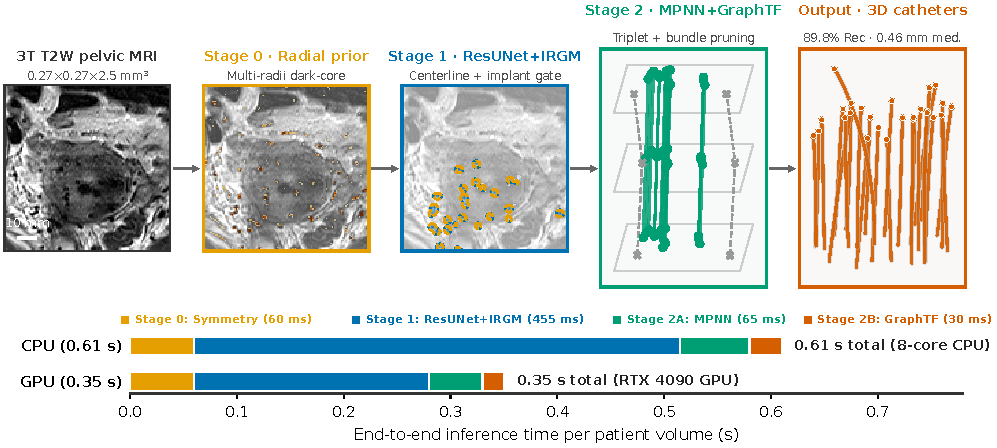
\includegraphics[width=1\linewidth,height=\textheight,keepaspectratio]{../reports/figures/fig1_pipeline_overview.pdf}
\caption{\textbf{Combining a physical 3D dark-core symmetry prior with
multi-scale graph learning turns a 45--50 minute manual tracing
bottleneck into a 4.15 s automatic reconstruction in 3D Slicer.}
\textbf{(a) Clinical bottleneck vs.~NeedleFinder 2026 workflow:} In
MRI-guided interstitial gynecologic brachytherapy, 15 to 30 thin 6F (2.0
mm) plastic catheters are inserted through a perineal template and
vaginal obturator into the high-risk tumor target (HR-CTV). Because
plastic tubes contain no mobile protons, they appear only as tiny signal
voids on 3T T2-weighted MRI (\(\Delta z = 1.6\text{--}5.0\text{ mm}\)),
requiring 45 to 50 minutes of manual slice-by-slice clicking while the
patient waits under anesthesia. \textbf{(b) Physical clues across three
scales:} (Clue 1, Stage 0) A catheter cross-section is a circular dark
core surrounded by brighter tissue across all six diameters
(\texttt{{[}+{]}}), whereas an organ border is a one-sided step edge
(\texttt{{[}-{]}}); (Clue 2, Stage 1) when two catheters touch
(\texttt{2.2\ mm} apart), binary segmentation masks merge into a single
blob (\texttt{{[}-{]}}), whereas regressing 2D Gaussian centerline peaks
keeps the two centers distinct (\texttt{{[}+{]}}); (Clue 3, Stage 2)
evaluating the full 15-to-30-catheter bundle together and profiling the
cranial termination in \(0.5\text{ mm}\) steps separates smooth
catheters (\texttt{{[}+{]}}) from bending pelvic vessels
(\texttt{{[}-{]}}). \textbf{(c) End-to-end visual progression on an
unseen test patient (Case 017, 26 expert reference trajectories):} From
left to right: native 3T T2W MRI (\texttt{10\ mm} scale bar); Stage 0
dark-core symmetry response \(S_0\) (\texttt{0.27\ s} Rust CPU); Stage 1
sub-pixel centerline peaks, shaft mask, and obturator contour
(\texttt{2.58\ s} CPU / \texttt{1.33\ s} GPU); Stage 2A/2B triplet
message-passing graph and collinear fragment stitching (\texttt{1.25\ s}
CPU / \texttt{1.05\ s} GPU); and Stage 2C 3D reconstructed bundle
(\texttt{vermilion\ solid}, \texttt{23} predicted) overlaid on expert
traces (\texttt{charcoal\ dashed}, \texttt{26} reference) with predicted
3D distal tips (\texttt{0.06\ s} CPU / \texttt{0.03\ s} GPU;
\texttt{4.15\ s} total CPU headless, \texttt{2.67\ s}
GPU).}\label{fig:overview}
\end{figure}

\subsection{A Quick Guide for Readers Outside Medical Physics or Machine
Learning}\label{a-quick-guide-for-readers-outside-medical-physics-or-machine-learning}

Because this paper bridges clinical radiation oncology, MRI physics, and
graph deep learning, we briefly define the core terms used throughout
the text:

\begin{itemize}
\tightlist
\item
  \textbf{Catheter (or needle), shaft, and tip.} We use \emph{catheter}
  and \emph{needle} interchangeably for the hollow 2 mm plastic tubes
  inserted into the tumor. The \textbf{shaft} is the main body of the
  tube passing through the tissue; the \textbf{tip} (or
  \emph{distal/cranial end}) is the deepest point the tube reaches
  inside the body, where the radioactive source stops first.
\item
  \textbf{Obturator and tandem.} Larger central plastic guides placed in
  the vagina (\emph{obturator}) and uterus (\emph{tandem}) around which
  the thinner interstitial catheters are arranged.
\item
  \textbf{Voxel, in-plane resolution, and slice thickness.} A 3D MRI
  scan is a stack of 2D horizontal cross-sections (\emph{axial slices}).
  Within each 2D slice (\emph{in-plane}), the image is sharp (pixel size
  0.31 to 0.88 mm). Between slices (along the vertical body axis,
  \(z\)), the spacing is much coarser (slice thickness 1.2 to 6.0 mm).
  This anisotropy explains why finding the sideways (\emph{in-plane})
  center of a catheter is easier than judging the exact height (\(z\))
  where its tip ends between two slices.
\item
  \textbf{Recall, precision, and F1 score.} \emph{Recall} is the
  percentage of real catheters the algorithm successfully finds.
  \emph{Precision} is the percentage of algorithm-reported tracks that
  correspond to a real catheter (rather than a false alarm on a blood
  vessel). The \emph{F1 score} is the harmonic mean of recall and
  precision; it is high only when the algorithm finds almost all real
  catheters while inventing very few false ones.
\item
  \textbf{Shaft error (\(E_{\text{shaft}}\)) and tip error
  (\(E_{\text{tip}}\)).} For every detected catheter that matches an
  expert trace (within 3.5 mm), \emph{shaft error} measures the sideways
  distance (in mm) between the automatic curve and the expert curve
  along their shared length. \emph{Tip error} measures the 3D distance
  (in mm) between the predicted deepest tip and the expert's deepest
  tip.
\item
  \textbf{Strictly nested cross-validation (out-of-fold evaluation).} To
  test our models on all 54 patients without ever testing on data used
  for training or tuning, we split the 54 patients into 5 outer groups
  (folds). In each round, 43 or 44 patients are used for training and
  tuning (via an internal 80/20 split or 5-fold inner cross-fitting),
  and the remaining 10 or 11 patients are held in a locked vault and
  evaluated \emph{once}. Every patient is thus evaluated strictly
  ``out-of-fold'' (as an unseen patient).
\item
  \textbf{Dosimetric metrics (\(D_{90}\), \(D_{2\text{cc}}\), and 3D
  \(\gamma\)).} In brachytherapy planning, \(D_{90}\) is the minimum
  radiation dose covering 90\% of the high-risk tumor volume (which
  clinicians want to keep high), while \(D_{2\text{cc}}\) is the dose to
  the most-irradiated \(2\text{ cm}^3\) of a nearby healthy organ like
  the bladder or rectum (which clinicians want to keep low). The 3D
  \emph{gamma (\(\gamma\)) pass rate} (\(2\%/2\text{ mm}\)) measures the
  percentage of points in the 3D volume where the dose planned on
  automatic catheters agrees with the reference plan within 2\% dose or
  2 mm distance.
\end{itemize}

\subsection{Why Existing Approaches Fall Short on T2-Weighted
MRI}\label{why-existing-approaches-fall-short-on-t2-weighted-mri}

Over the past decade, automatic catheter reconstruction has evolved
through three generations (reviewed in (Sargazi \emph{et al.}, 2026;
Vijayan \emph{et al.}, 2026)):

\textbf{Generation 1: Geometric and mechanical tracking from manual
clicks (2012--2019).} Early work in our Brigham and Women's Hospital
(BWH) program introduced image-guided catheter tracking in the Advanced
Multimodality Image Guided Operating (AMIGO) suite (Kapur \emph{et al.},
2012; Chen and Egger, 2014). Starting from a manual click at each
catheter tip, cone-search trackers (Pernelle \emph{et al.}, 2013) and
mechanical rod-and-spring splines (Mastmeyer \emph{et al.}, 2017a;
Mastmeyer \emph{et al.}, 2017b) achieved \textasciitilde1.4--1.5 mm
accuracy on T2W MRI. Similar geometry-guided or template-registered
methods work well on CT, ultrasound, or rigid applicators (W \emph{et
al.}, 2013; Dise \emph{et al.}, 2015; J \emph{et al.}, 2015; Hrinivich
\emph{et al.}, 2019; Deufel \emph{et al.}, 2020; Zheng \emph{et al.},
2021). However, they still require a human to click every catheter tip
first, and they often lose track when catheters bend sharply or cross
dark vessels.

\textbf{Generation 2: 3D voxel segmentation with clustering
(2019--2026).} To eliminate manual clicks, Zaffino \emph{et al.} (2019)
trained a 3D U-Net on 50 BWH gynecologic MRI scans to classify every
voxel as ``catheter'' or ``background,'' then grouped the segmented
voxels into tubes using density clustering (DBSCAN). Subsequent studies
applied 3D U-Nets and nnU-Net (Isensee \emph{et al.}, 2021) across CT,
ultrasound, and prostate or marker-assisted MRI (Jung \emph{et al.},
2019b; Jung \emph{et al.}, 2019a; Andersén \emph{et al.}, 2020; Dai
\emph{et al.}, 2020; Li \emph{et al.}, 2020; Wang \emph{et al.}, 2020;
Zhang \emph{et al.}, 2020a; Zhang \emph{et al.}, 2020b, 2020c; Zhang
\emph{et al.}, 2020d; Hu \emph{et al.}, 2021; Liu \emph{et al.}, 2022;
Shaaer \emph{et al.}, 2022; Weishaupt \emph{et al.}, 2022; Xie \emph{et
al.}, 2023; Aleong \emph{et al.}, 2024; Wang \emph{et al.}, 2024; Zhou
\emph{et al.}, 2024; Goulet \emph{et al.}, 2025; Kostoulas \emph{et
al.}, 2025; Moradi \emph{et al.}, 2025; Quetin \emph{et al.}, 2025; Kim
\emph{et al.}, 2026). Yet even when trained with topology-preserving
losses such as centerline-Dice (clDice) (Hu \emph{et al.}, 2019; Shit
\emph{et al.}, 2021; Kirchhoff \emph{et al.}, 2024), pure voxel
segmentation suffers from two fundamental failure modes on T2W MRI:

\begin{enumerate}
\def\labelenumi{\arabic{enumi}.}
\tightlist
\item
  \emph{Over-fragmentation:} If a catheter's dark void fades on even a
  single slice due to partial-volume averaging, the segmented mask
  breaks into 2 to 4 separate pieces.
\item
  \emph{Touching catheters and vascular false alarms:} When two
  catheters touch (\emph{catheter adhesion}), their voxel masks merge
  into a single blob; meanwhile, dark pelvic veins and tissue edges are
  segmented as dozens of short false catheters.
\end{enumerate}

\textbf{Generation 3: Structure-aware tracking, gap-bridging, and
uncertainty-weighted fitting (2020--2026).} To mitigate segmentation
breaks on MRI, Dai \emph{et al.} (2020) introduced a deeply supervised
3D attention-gated U-Net with axial total-variation (TV) continuity
regularization, Kostoulas \emph{et al.} (2025) combined a 3D residual
U-Net with iterative collinear gap-bridging and false-part pruning, and
Aleong \emph{et al.} (2024) and Kim \emph{et al.} (2026) leveraged
5-model epistemic uncertainty ensembles and inverse-variance-weighted
polynomial trajectory fitting. On pelvic CT, Xiao \emph{et al.} (2026a,
2026b) addressed catheter adhesion by combining an implant-region gating
module with 3D Hough initialization and synchronous slice-to-slice
tracking. In computer vision, message-passing graph networks (Brasó and
Leal-Taixé, 2020; Ben-Haim and Riklin Raviv, 2022; Shit \emph{et al.},
2022), keypoint regression (Zhou \emph{et al.}, 2026), and
synthetic-to-real transfer (Arapi \emph{et al.}, 2023) have similarly
improved curvilinear tracking. However, a mask-driven tracker applied to
T2W MRI without a physical circular-symmetry prior or whole-bundle
reasoning still trusts the underlying segmentation mask. Dark pelvic
veins inside the implant region are tracked as catheters. The tracker
has no mechanism to ask whether the resulting collection of 25
trajectories makes sense \emph{together} as a physical implant, nor to
resolve sub-slice tip terminations on thick MRI slices. (Hardware-based
electromagnetic or active MR tracking avoids image ambiguity (Mehrtash
\emph{et al.}, 2014; Wang \emph{et al.}, 2015; Arcos \emph{et al.},
2017; Dürrbeck \emph{et al.}, 2022; Cantin \emph{et al.}, 2024; Deufel
\emph{et al.}, 2024; Beaulieu \emph{et al.}, 2025; Roumeliotis \emph{et
al.}, 2026), but requires specialized catheters and operating-room
hardware.)

\subsection{How NeedleFinder 2026 Solves These
Problems}\label{how-needlefinder-2026-solves-these-problems}

NeedleFinder 2026 bridges all three generations on the complete
54-patient, 1,063-catheter BWH gynecologic MRI cohort---to our knowledge
the largest annotated clinical MRI dataset for interstitial
brachytherapy to date (Figure \ref{fig:overview}). Each stage of our
architecture is designed to solve a specific failure mode of prior work:

\begin{enumerate}
\def\labelenumi{\arabic{enumi}.}
\tightlist
\item
  \textbf{Physics before learning (Stage 0):} Before any neural network
  runs, an analytical 3D circular dark-core symmetry filter separates
  round dark cross-sections (catheters and vessels) from one-sided dark
  boundaries (fascial planes and organ walls), while an automatic
  template-plane locator finds the base of the implant without needing
  manual bounding boxes.
\item
  \textbf{Centerline peaks and self-supervised pelvic pre-training
  (Stage 1):} Instead of relying on binary masks alone, our
  native-resolution 3D U-Net regresses sharp sub-pixel \emph{centerline
  peaks} and \emph{3D tangent directions}---so two touching catheters
  still produce two distinct peaks. To prevent the network from
  confusing pelvic veins with catheters, we pre-train it on 51 external
  pelvic MRI volumes (from 50 subjects) by injecting realistic synthetic
  catheter voids while explicitly penalizing real pelvic vessels and
  fascia as hard negatives, and then fine-tune it using consensus traces
  from two independent expert teams.
\item
  \textbf{Graph linking, fragment stitching, bundle-level reasoning, and
  1D tip localization (Stage 2):} A triplet message-passing graph
  network links slice detections while penalizing sharp kinks, and a
  geometric stitcher reconnects catheter fragments separated by
  1-to-3-slice signal dropouts. Next, a bundle graph transformer
  evaluates all candidate trajectories simultaneously in the context of
  the whole implant. Finally, a dedicated 1D axial neural network
  samples a fine \(0.5\text{ mm}\) multi-scale profile along the end of
  each trajectory to pinpoint the exact distal tip and output a
  calibrated split-conformal uncertainty interval, optionally fused with
  sub-voxel inverse-variance-weighted polynomial refinement (Aleong
  \emph{et al.}, 2024; Kim \emph{et al.}, 2026), axial TV continuity
  (Dai \emph{et al.}, 2020), and iterative multi-segment gap-bridging
  (Kostoulas \emph{et al.}, 2025).
\end{enumerate}

Beyond geometric benchmarking against five peer-reviewed MRI/curvilinear
methods and one recent tracking preprint reproduced on the identical
nested splits, we evaluate NeedleFinder 2026 across four clinical
translation dimensions: (i) three-cornered-hat observer adjudication
against two human expert teams and paired post-implant CT scans; (ii)
AAPM TG-43U1 \(^{192}\text{Ir}\) radiation dosimetry; (iii)
uncertainty-guided clinician tip triage; and (iv) zero-shot
generalization to needle-free pelvic MRI, 3T prostate brachytherapy MRI,
secondary MRI pulse sequences, serial intra-procedural insertion scans,
and pelvic CT. Directly extending our group's multi-planar mechanical
rod tracking in \emph{Medical Image Analysis} (Mastmeyer \emph{et al.},
2017b) and 3D U-Net voxel clustering in \emph{Physics in Medicine \&
Biology} (Zaffino \emph{et al.}, 2019) to the full 54-patient AMIGO
cohort, this study simultaneously addresses open challenges across three
communities: in \textbf{brachytherapy}, enabling marker-free T2W
MRI-only catheter digitization and dosimetrically calibrated tip
verification; in \textbf{computer vision and geometric deep learning},
resolving touching curvilinear tubes (\(\le 3.0\text{ mm}\)) under
extreme axial anisotropy (\(\Delta z / \Delta x\) up to \(15\times\))
via hybrid 3D CNN peak regression, triplet message-passing, and
whole-bundle graph transformers; and in \textbf{image-guided therapy},
delivering 4.15 s GPU-free reconstruction in 3D Slicer alongside 1.31 s
causal 4D intra-procedural tracking and in-vivo tissue-push
biomechanics.

\FloatBarrier

\section{Patient Cohorts and Clinical
Datasets}\label{patient-cohorts-and-clinical-datasets}

\begin{table}[tbp]
\centering
\begin{threeparttable}
\caption{\textbf{Clinical imaging cohorts and evaluation protocols.}
Primary evaluation uses strictly nested $5\times 5$ patient-level out-of-fold (OOF) cross-validation with 100\,\% reference-free axial cropping (\texttt{k\_lim\_auto}) on 54 clinical 3T T2W MRI datasets from Brigham and Women's Hospital (BWH AMIGO).}
\label{tbl:cohorts}
\footnotesize
\setlength{\tabcolsep}{1.8pt}
\begin{tabular}{@{}L L R R L L L@{}}
\toprule
Cohort / Subset & Source & {Pts} & {Cath.} & {XY (mm)} & {$\Delta z$ (mm)} & {Evaluation role}\\
\midrule
BWH GYN full cohort\tnote{a} & BWH (3T T2W) & 54 & 1063 & $0.31\text{--}0.88$ & $1.2\text{--}6.0$ & Nested $5\times 5$ OOF benchmark\\
\quad Long shafts (primary) & BWH (3T T2W) & 54 & 759 & $0.31\text{--}0.88$ & $1.2\text{--}6.0$ & Full-depth active dwell shafts\\
\quad Short / obturator (secondary) & BWH (3T T2W) & 54 & 304 & $0.31\text{--}0.88$ & $1.2\text{--}6.0$ & Partial-FOV \& template tracks\\
\quad Adhesion subgroup\tnote{b} & BWH (3T T2W) & 23 & 571 & $0.31\text{--}0.88$ & $1.2\text{--}6.0$ & Touching / crossing shaft test\\
Dual-observer subset\tnote{c} & BWH (3T T2W) & 40 & 723 & $0.31\text{--}0.88$ & $1.2\text{--}6.0$ & Inter-observer floor (\texttt{CY+HT}, \texttt{LB}/\texttt{AMe})\\
External SSL \& specificity\tnote{d} & MSD + BWH & 50 (51) & 0 & $0.47\text{--}0.88$ & $1.6\text{--}4.8$ & 3D SSL (51) \& 0-needle test (48)\\
Prostate 3T implant (\texttt{Case 100})\tnote{e} & BWH (3T T2W) & 1 (1) & 14 & $0.47$ & $1.6$ & Zero-shot cross-organ transfer\\
Secondary GYN MRI sequences\tnote{e} & BWH (wbSSFP/2D) & 54 (243) & 929 & $0.31\text{--}0.94$ & $2.0\text{--}6.0$ & Zero-shot multi-sequence test\\
4D serial insertion (\texttt{Cases 68--71})\tnote{e} & BWH (3T T2W) & 4 (23) & 108 & $0.31\text{--}0.75$ & $1.6\text{--}3.0$ & Causal 4D tracking \& biomechanics\\
Paired post-implant Pelvic CT\tnote{e} & BWH (Pelvic CT) & 38 (40) & 801 & $0.49\text{--}0.98$ & $1.25\text{--}2.5$ & CT adjudication \& cross-modality\\
\bottomrule
\end{tabular}
\begin{tablenotes}[flushleft]\footnotesize
\item[a] Consolidated superset of the cohorts of Pernelle \emph{et al.}\ (2013, 10 patients) and Zaffino \emph{et al.}\ (2019, 50 patients), extended with new implants; 9--42 reference trajectories per patient (20 standard-resolution $320\times256$ scans and 34 high-resolution $640\times416$ / $768\times768$ scans). In the Pts column, parentheses indicate total volumes when multiple scans per subject are analysed.
\item[b] Severe catheter-adhesion subgroup: the 23/54 patients in which $\ge 4$ long or $\ge 6$ total reference catheters pass within $\le 3.0$\,mm of another catheter on shared axial slices. All 571 catheters of these patients are evaluated; 191 of them (166 long) lie within $3.0$\,mm of a neighbour (233 across the whole cohort).
\item[c] All 40/40 dual-traced clinical scenes independently contoured by two expert medical physics teams (\texttt{CY+HT}: 723 total trajectories = 505 \texttt{CY} long + 218 \texttt{HT} short/obturator; \texttt{LB}/\texttt{AMe}: 513 trajectories, with 465 consensus-fused with \texttt{CY}, 12 matched to \texttt{HT} within $\le 5.0$\,mm [$11$ within $\le 3.5$\,mm], and $36$ unique \texttt{LB}/\texttt{AMe} trajectories forming the $759$-trajectory union).
\item[d] Fifty-one external pelvic 3T T2W MRI volumes from 50 distinct subjects: 48 public CC-BY-SA 4.0 volumes from MSD \texttt{Task05\_Prostate} ($0.60\text{--}0.75$\,mm in-plane, $3.0\text{--}4.0$\,mm slices; zero implanted catheters, evaluated for false-positive specificity) plus 3 non-benchmark BWH pelvic T2W volumes from 2 distinct subjects (\texttt{Case 061} [2 series, $0.88$\,mm in-plane, $4.8$\,mm slices] and \texttt{Case 100 Prostate} [1 series, $0.47$\,mm in-plane, $1.6$\,mm slices], zero patient overlap with the 54 benchmark cases) used for self-supervised 3D U-Net pre-training.
\item[e] Cross-domain validation cohorts summarized in Table~\ref{tbl:clinical_summary} and detailed in Appendix~D (Table~\ref{tbl:app_generalization}): zero-shot 3T prostate brachytherapy MRI (\texttt{Case 100}, 14 plastic needles); 243 secondary MRI volumes across the 54 sessions (including 2 \texttt{3D wbSSFP} volumes [47 catheters] and 49 thick-slice \texttt{2D AX TSE T2} volumes [882 physically visible catheters]); 23 sequential 4D intra-procedural insertion scans across 4 patients (\texttt{Cases 68--71}, 108 final catheters); and 40 post-implant Pelvic CT scans (38 paired with benchmark MRI patients, 801 reference catheters).
\end{tablenotes}
\end{threeparttable}
\end{table}


Table \ref{tbl:cohorts} summarizes all clinical benchmark,
inter-observer, external pre-training, and cross-domain validation
cohorts analyzed in this study:

\begin{enumerate}
\def\labelenumi{\arabic{enumi}.}
\tightlist
\item
  \textbf{Primary gynecologic MRI cohort (54 patients, 1,063
  catheters).} We analyzed 54 intraoperative 3T T2W turbo spin-echo MRI
  volumes acquired during MRI-guided interstitial gynecologic
  brachytherapy in the AMIGO suite at Brigham and Women's Hospital
  (Harvard Medical School, Boston, MA, USA) under Institutional Review
  Board approval (Pernelle \emph{et al.}, 2013; Mastmeyer \emph{et al.},
  2017b; Zaffino \emph{et al.}, 2019). This cohort consolidates the 48
  recoverable cases from our 2013 and 2019 studies with 6 newly curated
  implants. Patients were implanted using a Syed--Neblett perineal
  template surrounding a central vaginal obturator
  (\(R_{\text{obt}} \approx 10\text{--}15\text{ mm}\)) and scanned with
  6F polymeric interstitial catheters (with plastic or non-ferromagnetic
  obturators in situ, creating a proton-density signal void and mild
  interface susceptibility contrast on T2W MRI). Expert medical
  physicists traced 1,063 reference trajectories (9 to 42 per patient).
  These comprise \textbf{759 full-depth interstitial shafts} (which
  penetrate into the tumor to carry the active radiation dwell
  positions; archive code \texttt{CY} in Table \ref{tbl:cohorts}) and
  \textbf{304 shorter auxiliary tracks} sitting inside the central
  vaginal obturator lumen (including any central tandem or internal
  obturator guide channels, which Stage 1 also masks at the outer
  obturator rim via \(P_{\text{obt}}\)) or only partially entering the
  field of view (archive code \texttt{HT}). Twenty scans were acquired
  at standard in-plane resolution (\(320 \times 256\) matrix,
  \(0.75\text{--}0.88\text{ mm}\) pixels) and 34 at high resolution
  (\(640 \times 416\) to \(768 \times 768\) matrix,
  \(0.31\text{--}0.55\text{ mm}\) pixels), with slice thickness ranging
  from \(1.2\text{ to }6.0\text{ mm}\).
\item
  \textbf{Severe catheter-adhesion subgroup (23 patients, 571
  catheters).} Following Xiao \emph{et al.} (2026a), we identified the
  23 patients in whom catheters are tightly packed or touching---defined
  as having at least 4 long shafts (or at least 6 total catheters) that
  pass within \(\le 3.0\text{ mm}\) in-plane centerline distance of a
  neighboring catheter on shared slices. All 571 catheters in these 23
  patients are evaluated together (191 of them touch a neighbor within
  \(\le 3.0\text{ mm}\), out of 233 such touching catheters across all
  54 patients).
\item
  \textbf{Dual-expert inter-observer cohort (40 patients).} Forty of the
  54 scans were traced independently by two separate expert groups:
  \textbf{Expert Team 1} (723 trajectories: 505 long shafts and 218
  short obturator tracks) and \textbf{Expert Team 2} (archive code
  \texttt{LB/AMe}: 513 trajectories, of which 460 are long shafts).
  Across these 40 scans, 424 long-shaft pairs (and 476 all-catheter
  pairs) match one-to-one within \(3.5\text{ mm}\) between the two human
  teams, while their de-duplicated union contains 759 distinct
  trajectories (\(723\) from Team 1 plus \(36\) additional catheters
  traced only by Team 2).
\item
  \textbf{External pelvic MRI cohort for self-supervised pre-training
  and false-alarm testing (51 volumes from 50 subjects).} To pre-train
  our 3D network on pelvic anatomy and test false-alarm rates on the 48
  public scans containing \emph{zero} catheters, we assembled 51
  strictly external 3T T2W pelvic MRI volumes having zero patient
  overlap with the 54 benchmark cases: all \textbf{48 public prostate
  MRI scans} from the Medical Segmentation Decathlon
  (\texttt{MSD\ Task05\_Prostate} (Antonelli \emph{et al.}, 2022);
  \(0.60\text{--}0.75\text{ mm}\) pixels, \(3.0\text{--}4.0\text{ mm}\)
  slices) plus \textbf{3 non-benchmark BWH pelvic T2W volumes} from two
  separate patients (\texttt{Case\ 061} {[}2 series{]} and
  \texttt{Case\ 100\ Prostate} {[}1 series{]}).
\item
  \textbf{Cross-organ, multi-sequence, 4D insertion, and paired CT
  validation cohorts.} To test how well the gynecologic-trained pipeline
  generalizes without retraining (Table \ref{tbl:cohorts}, bottom four
  rows; Table \ref{tbl:clinical_summary}, Part D; Appendix D, Table
  \ref{tbl:app_generalization}), we evaluated: (i) a clinical 3T T2W
  \textbf{prostate brachytherapy implant} (\texttt{Case\ 100}, 14
  plastic needles); (ii) \textbf{243 secondary MRI volumes} acquired
  during the 54 gynecologic procedures, including 3D balanced
  steady-state free precession (\texttt{3D\ wbSSFP\ /\ True-FISP}, 2
  volumes, 47 catheters), 12 post-contrast axial T1 VIBE volumes (217
  catheters), and 49 thick-slice 2D axial T2W (\texttt{2D\ AX\ TSE\ T2},
  \(2.4\text{--}6.0\text{ mm}\) slices, 882 physically visible
  catheters) scans; (iii) \textbf{23 serial 4D intra-procedural MRI
  scans} acquired across 4 patients (\texttt{Cases\ 68–71}, 5 to 7
  sequential scans per patient as needles were progressively inserted,
  108 final catheters); and (iv) \textbf{40 post-implant pelvic CT
  volumes} (38 of them paired directly with benchmark MRI patients, 801
  reference catheters).
\end{enumerate}

\FloatBarrier

\section{Architecture of NeedleFinder
2026}\label{architecture-of-needlefinder-2026}

A human physicist tracing catheters on MRI uses three kinds of clues in
sequence: first, looking for small round dark spots on each 2D slice;
second, checking whether those dark spots line up across adjacent
slices; and third, verifying that the full collection of 15 to 30 curves
forms a plausible implant bundle and stopping each curve where the dark
void disappears at the tip. NeedleFinder 2026 mirrors this exact
hierarchy in three stages (Figures \ref{fig:overview} and
\ref{fig:arch}).

\subsection{Stage 0: Physical Dark-Core Symmetry and Automatic Template
Cropping}\label{stage-0-physical-dark-core-symmetry-and-automatic-template-cropping}

\textbf{The physical intuition.} Why do standard neural networks confuse
muscle borders and organ walls with catheters? Because both are dark on
T2W MRI. However, their \emph{geometry} is different: a muscle border is
a dark edge with bright tissue on one side and dark tissue on the other,
whereas a catheter cross-section is a tiny dark core surrounded by
brighter tissue in \emph{every} direction.

Stage 0 turns this geometric observation into a fast 3D filter
\(S_0(x,y,z)\) with no learned parameters, implemented in multi-threaded
native Rust. At every voxel \(\mathbf{p}\) on axial slice \(z\), we
sample six diameters passing through \(\mathbf{p}\) at angles
\(\theta_d = d\pi/6\) (\(d \in \{0, \dots, 5\}\)) across four physical
radii \(r \in \mathcal{R} = \{1.35, 1.85, 2.5, 3.3\}\text{ mm}\)
(converted to pixels using the scan's in-plane spacing). Along each
diameter \(d\) and radius \(r\), we take the \emph{darker} of the two
opposite ring points:
\[m_{d,r} = \min\!\big(I(\mathbf{p} + r\mathbf{u}_d),\; I(\mathbf{p} - r\mathbf{u}_d)\big).\]
If \(\mathbf{p}\) sits on a one-sided edge, at least one end of the
diameter remains dark, keeping \(m_{d,r}\) small. We then sort the six
directional values (\(m_{(1),r} \le \dots \le m_{(6),r}\)) and compute a
robust ring brightness that requires the surrounding tissue to be bright
in almost all directions while tolerating a single dark neighbor (such
as a touching twin catheter):
\[S_{\text{ring}}(\mathbf{p}) = \max_{r \in \mathcal{R}} \big[0.45\, m_{(2),r} + 0.55\, m_{(3),r}\big].\]
Combining this positive ring-to-core contrast with the relative darkness
of the \(3 \times 3\) smoothed center intensity
\(\bar{I}_{3\times 3}(\mathbf{p}) \in [0, 1]\) yields the raw dark-core
symmetry score,
\[S_0(\mathbf{p}) \propto \max\!\big(0,\; S_{\text{ring}}(\mathbf{p}) - \bar{I}_{3\times 3}(\mathbf{p})\big)\cdot\big[1 - \bar{I}_{3\times 3}(\mathbf{p})\big],\]
which is normalized to \([0, 1]\) per volume. Because \(S_0\) takes the
maximum over radii up to \(3.3\text{ mm}\) and uses the second- and
third-darkest of the six directional values, it is, by construction,
tolerant of realistic oblique catheter tilt
(\(\alpha \le 25^\circ\text{--}30^\circ\) relative to the slice normal,
where the in-plane elliptical cross-section elongates by only
\(\sec\alpha \le 1.15\); see Appendix A for the formal tilt-invariance
derivation). On very thick slices (\(\Delta z = 4\text{--}6\text{ mm}\))
where steep tilt causes stronger partial-volume elongation, we first
upsample the volume along \(z\) to \(1.6\text{ mm}\) spacing and rely on
Stage 2A fragment stitching to bridge dimmed slices.

\textbf{Automatic reference-free cropping of the template plane.} Below
the patient's perineum, the inferior slices of the MRI scan contain
outside air and the plastic needle-guiding template. Previously,
pipelines relied on manually drawn bounding boxes to crop out these
bottom slices, which is unavailable in a fully automatic workflow and
occasionally clipped tilted templates too high---cutting off the bases
of 42 catheters across our cohort. We replaced this with a
reference-free axial template locator. After standardizing the volume to
caudo-cranial slice ordering via its DICOM/NRRD direction cosines, the
locator scans upward from the inferior boundary and detects the
step-change in 90th-percentile soft-tissue intensity alongside the
emergence of clustered dark-core candidates (\(S_0\)) within the central
field of view. Across all 54 patients, it places the crop boundary a
median of \(2.0\) slices deeper than the manually drawn boxes (mean
\(1.91\) slices deeper, IQR \(1.0\); \(64.1\) vs.~\(62.2\) active slices
on average), eliminating all 42 in-field-of-view base truncations and
preserving \textbf{100.0\% of in-field-of-view catheter length}
(\(99.65\%\) of total unclipped catheter length) without ever consulting
manual annotations. Stage 0 and automatic cropping run in \textbf{0.27
s} per volume on a 24-core CPU (0.07 s on standard scans, 0.38 s on
high-resolution scans).

\begin{figure}
\centering
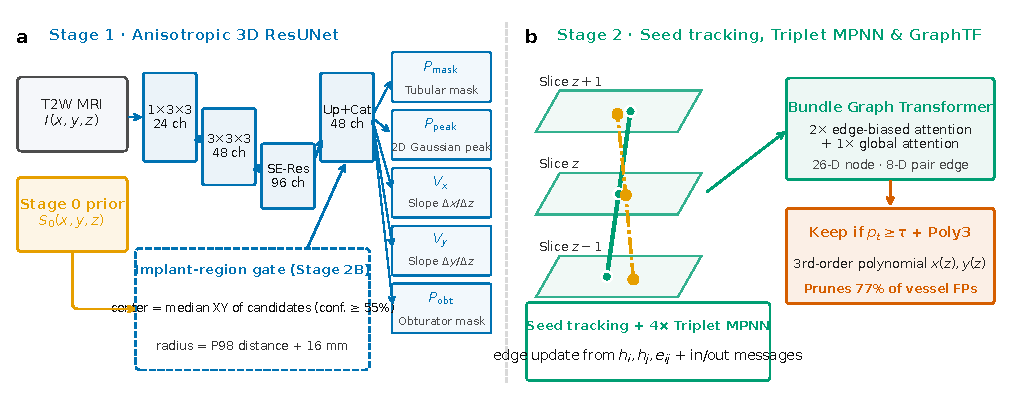
\includegraphics[width=1\linewidth,height=\textheight,keepaspectratio]{../reports/figures/fig2_architecture_modules.pdf}
\caption{\textbf{Four-stage physical and neural mechanism of
NeedleFinder 2026.} \textbf{(a) Stage 0 analytical dark-core prior and
template auto-crop:} At each voxel \(\mathbf{p}\), six diameters
(\(\theta_d = d\pi/6\)) across four physical radii
(\(r \in [1.35, 3.30]\text{ mm}\)) evaluate two-sided radial contrast
\(\min(I(\mathbf{p}+r\mathbf{u}_d), I(\mathbf{p}-r\mathbf{u}_d)) - I(\mathbf{p})\);
the rank-2/rank-3 order statistic \(S_0(\mathbf{p})\) suppresses
one-sided organ borders while tolerating a touching neighbor, and
\texttt{k\_lim\_auto} locates the caudal template entry slice
automatically (\texttt{0.27\ s} Rust CPU). \textbf{(b) Stage 1
native-resolution anisotropic 3D ResUNet (\texttt{NeedleUNet3D}):}
Operating directly on the native voxel grid (\texttt{1×3×3} in-plane
stem and SE-Res blocks), the network is pre-trained on 51 external
pelvic MRI volumes (penalizing real vessels and fascia as hard
negatives) and fine-tuned on dual-expert consensus traces to predict
four heads: tubular mask (\(P_{\text{mask}}\)), sub-pixel centerline
peaks (\(P_{\text{peak}}\)), local 3D slope (\(V_x, V_y\)), and
obturator mask (\(P_{\text{obt}}\)). \textbf{(c) Stage 2A \& 2B graph
tracking, collinear gap stitching, and bundle transformer:} A 4-layer
triplet message-passing network scores slice-to-slice bending angles
\(\cos\angle(\mathbf{v}_{ij}, \mathbf{v}_{jk})\) across \(z-1, z, z+1\);
a collinear stitcher bridges \(\le 20\text{ mm}\) signal dropouts; and a
26-D node / 8-D edge bundle graph transformer (pre-trained on
\texttt{SynthBrachy3T}) outputs calibrated confidence \(p_m \ge \tau\)
with reason codes. \textbf{(d) Stage 2C dedicated 1D axial tip localizer
and split-conformal sphere:} Sampling 91 steps (\(0.5\text{ mm}\) over
\([-25, +20]\text{ mm}\)) across 22 channels (24 in \texttt{4d}) along
the cranial tangent \(\hat{\mathbf{t}}\), a 3-block dilated 1D ResNet
(\(d=1,2,4\)) + 4-head self-attention predicts the stopping distribution
\(q_t\), sub-slice tip offset \(\Delta s\) (\texttt{2.27\ mm} median 3D
error), and split-conformal 3D tip radius
\(\hat{r}_{90} = \hat{q}_{90}\hat{\sigma}_{\text{tip}}\)
(\texttt{90.2\%} empirical coverage at 90\% nominal).}\label{fig:arch}
\end{figure}

\subsection{Stage 1: Native-Resolution 3D U-Net with Self-Supervised and
Multi-Rater
Learning}\label{stage-1-native-resolution-3d-u-net-with-self-supervised-and-multi-rater-learning}

\textbf{Why native resolution and multiple output heads matter.} Many 3D
medical segmentation pipelines first resample every scan to coarser,
near-isotropic voxels such as \(1 \times 1 \times 1\text{ mm}^3\). For a
2 mm catheter imaged at \(0.35\text{ mm}\) pixel resolution, resampling
blurs the sharp dark core into the surrounding tissue. Conversely,
applying a standard \(3 \times 3 \times 3\) convolution directly on the
native grid mixes features across up to 18 mm vertically (\(z\)) but
only 1 mm horizontally (\(x, y\)).

Our Stage 1 network (Figure \ref{fig:arch}a) therefore operates directly
on the native voxel grid using an anisotropic 3D residual U-Net with
squeeze-and-excitation channel attention at four scales (24, 48, 96, and
144 channels). Crucially, it pools spatially \emph{only in-plane}
(\(x, y\)) at the first two scales so that thick axial slices are never
compressed early. The network takes six input channels---normalized T2W
intensity, Stage 0 dark-core symmetry \(S_0\), ring contrast, smoothed
intensity, normalized axial height \(z\), and radial distance from the
scan center---and predicts four complementary outputs:

\begin{enumerate}
\def\labelenumi{\arabic{enumi}.}
\tightlist
\item
  \textbf{Tubular mask (\(P_{\text{mask}}\)):} The probability that a
  voxel lies within a catheter cross-section (trained with focal binary
  cross-entropy, up-weighted 19-fold on catheter voxels and on false
  Stage 0 vessel peaks, plus soft Dice loss).
\item
  \textbf{Sub-pixel centerline peak (\(P_{\text{peak}}\)):} A narrow 2D
  Gaussian heatmap (\(\sigma = 0.70\text{ mm}\)) centered on the exact
  intersection of each catheter with the slice (trained with
  peak-weighted mean-squared error). \textbf{Why this matters:} When two
  catheters touch, their binary masks (\(P_{\text{mask}}\)) merge into
  one blob, but their two centerline peaks (\(P_{\text{peak}}\)) remain
  distinct.
\item
  \textbf{Local 3D direction field
  (\(V_x, V_y = \Delta x/\Delta z, \Delta y/\Delta z\)):} The local tilt
  of the catheter as it passes from slice to slice (trained with smooth
  \(L_1\) loss and an axial consistency penalty), telling the tracker
  where to look on the next slice.
\item
  \textbf{Obturator segmentation (\(P_{\text{obt}}\)):} A dedicated mask
  for the large central vaginal obturator
  (\(R_{\text{obt}} \approx 10\text{--}15\text{ mm}\)) and its outer
  cylindrical plastic wall, preventing its curved dark rim from
  generating false peripheral needle detections while allowing central
  tandem or internal obturator guide channels (\texttt{HT}) to be
  identified and distinguished from full-depth interstitial shafts
  (\texttt{CY}).
\end{enumerate}

\textbf{How we teach Stage 1 to ignore blood vessels and noisy
single-rater labels.} We introduce two training innovations for Stage 1:

\begin{itemize}
\tightlist
\item
  \textbf{Self-supervised pre-training on 51 external pelvic MRI scans
  with anatomical hard negatives.} Before training on any benchmark
  brachytherapy patient, we pre-train the 3D U-Net for 45 epochs across
  the 51 external needle-free pelvic MRI volumes (48 public MSD prostate
  scans + 3 non-benchmark BWH pelvic scans). In each training step, we
  digitally inject 8 to 20 realistic synthetic 3D catheter
  trajectories---curved dark cores with partial-volume bright rims and
  random signal dropouts---while simultaneously masking random 3D tissue
  patches for reconstruction. Because 50 of these 51 external scans
  contain \emph{zero} real catheters, \textbf{every real pelvic blood
  vessel, bowel loop, or fascial border that triggers a high Stage 0
  symmetry score (\(S_0 > 0.25\)) outside the synthetic tubes serves as
  an anatomical hard negative} (the one prostate implant scan
  contributes its 14 unlabeled needles as background, which we accept as
  label noise). The network is thus pushed to separate a plastic
  catheter void from a pelvic vein before it ever sees the benchmark
  cohort.
\item
  \textbf{Multi-rater consensus supervision.} On the 40 training scans
  traced by both human expert teams, training on a single team's
  annotations penalizes the network whenever it finds a real catheter
  that Team 1 overlooked but Team 2 traced, and passes along
  single-observer clicking jitter. Within each outer training fold
  (never touching test patients), we pair matching trajectories between
  Team 1 and Team 2 (\(\le 3.5\text{ mm}\), \(n = 465\) pairs) and
  supervise Stage 1 along their precision-weighted consensus centerline
  (weight \(1.15\)). Catheters traced only by Team 1 receive weight
  \(1.00\), and additional catheters traced only by Team 2 (\(n = 35\)
  after excluding \(465\) primary-matched and \(13\)
  obturator-overlapping traces; this training-time match pairs each Team
  2 trace, clipped to the automatic axial crop, with a Team 1 long shaft
  only, so its counts differ slightly from the evaluation-time pairing
  of all unclipped traces of both teams in the cohort description above,
  476 pairs) receive soft positive weight \(0.55\) instead of being
  treated as background false alarms.
\item
  \textbf{Inner 5-fold ensembling and 4-view test-time augmentation.}
  Within each outer training fold, we train 5 inner-fold Stage 1 models
  with rich 3D MRI augmentations (random 3D bias fields, slice-thickness
  blurring, slice dropouts, and flips) and average their predictions
  across four flip symmetries (\(I, X, Y, XY\)) at inference.
\end{itemize}

\subsection{Stage 2: Graph Tracking, Fragment Stitching, Bundle Scoring,
and 1D Tip
Localization}\label{stage-2-graph-tracking-fragment-stitching-bundle-scoring-and-1d-tip-localization}

Once Stage 1 has highlighted candidate catheter centers and directions
on every slice, Stage 2 solves three sequential geometric problems
(Figure \ref{fig:arch}c, d):

\subsubsection{Step 2A: Connecting slice detections and stitching split
fragments}\label{step-2a-connecting-slice-detections-and-stitching-split-fragments}

On each slice, local peaks of \(P_{\text{peak}}\) and \(S_0\) become
graph nodes (each described by 16 local image and direction features).
Directed edges connect nodes across 1 to 4 slices (up to
\(24\text{ mm}\) vertically) whenever their in-plane displacement agrees
with the Stage 1 direction field.

Why use a graph network alongside Kalman tracking instead of greedy
slice-to-slice linking alone? Because two consecutive links can each
look reasonable on their own yet form a sharp, unphysical kink when
joined together. First, a fast native C++17/Rust bidirectional Kalman
tracker traces candidate 3D paths from the Stage 0 and Stage 1 seeds in
both directions and merges near-duplicate paths within
\(1.65\text{--}2.05\text{ mm}\) while preserving genuinely touching twin
catheters. Second, a \textbf{4-layer triplet message-passing network}
(hidden width 64) scores every node and edge in the slice graph using
attention-weighted messages from both its incoming and outgoing
neighboring edges---explicitly rewarding smooth, collinear trajectories,
refining sub-pixel coordinates, and penalizing kinks.

Finally, our failure analysis of earlier pipelines revealed that
mid-shaft signal dropouts (where a catheter crosses a dark vessel or air
pocket over 1 to 3 slices) frequently split one physical catheter into a
lower fragment and an upper fragment---causing both a false-positive
extra fragment and a severe tip undershoot on the lower track. We
therefore added a \textbf{collinear split-fragment stitcher}: whenever a
lower track fragment ends and an upper fragment begins within an axial
gap of \(\le 20\text{ mm}\), and their linearly extrapolated positions
at the midpoint agree within \(\le 2.2\text{ mm}\) with matching 3D
slopes (\(\Delta \text{slope} \le 0.14\)), the two fragments are
seamlessly stitched into a single full-length candidate (creating 102
stitched full-length trajectories across the 54 patients).

\subsubsection{Step 2B: Judging the whole implant bundle
together}\label{step-2b-judging-the-whole-implant-bundle-together}

After Step 2A, the stitched candidate pool recovers \textbf{97.4\%} of
all real catheters (\(98.8\%\) of long shafts), and the greedily linked
Stage 2A tracks alone (Appendix B, Table \ref{tbl:app_ablation}) still
contain an average of 6.6 unmatched tracks per patient. How can the
algorithm tell a real catheter apart from a dark vein that happens to
look tubular over a few slices? By looking at the \textbf{whole bundle
at once}: real catheters enter through a common perineal template
corridor, run roughly parallel to the central obturator, maintain a
consistent spacing, and terminate along a coherent surface covering the
tumor.

We summarize each candidate trajectory by a 26-feature token (length,
straightness, Stage 0/1/2A confidence percentiles, entry position and
tilt relative to the bundle median, and tip contrast gradient) and
describe every pair of trajectories by 8 geometric interaction features
(minimum 3D clearance, shared-slice separation, angular divergence, and
overlap). A \textbf{bundle graph transformer} applies two layers of
edge-biased local attention between neighboring tracks followed by
global self-attention across the entire candidate bundle, outputting a
calibrated probability \(p_m \in [0, 1]\) that each candidate is a real
catheter. Candidates outside a self-calibrating implant radius (98th
percentile of high-confidence tracks plus \(16\text{ mm}\)) require a
higher confidence threshold to pass. To enable zero-shot and few-patient
learning, Stage 2B can also be pre-trained on \textbf{SynthBrachy3T}---a
physics-based generator of 300 simulated candidate bundles containing
realistic touching twins, short obturator channels, split fragments, and
vascular false alarms (detailed in Appendix A)---before fine-tuning on
the clinical training fold.

\subsubsection{Step 2C: Pinpointing the deepest tip, quantifying its
uncertainty, and fusing literature
priors}\label{step-2c-pinpointing-the-deepest-tip-quantifying-its-uncertainty-and-fusing-literature-priors}

Even when a catheter's shaft is traced to within half a millimeter,
finding its exact deepest (cranial) tip on thick-slice T2W MRI is
difficult: the dark void tapers off gradually across 2 to 6 mm thick
slices, or collides with dark bowel gas just above the uterus.

To resolve the tip with sub-slice precision, we built a
\textbf{dedicated 1D axial tip localizer} (Figure \ref{fig:arch}d).
Starting at the top of each candidate trajectory and continuing along
its 3D tangent direction, the network samples a \textbf{91-step 1D
profile} from \(-25.0\text{ mm}\) below the initial tip to
\(+20.0\text{ mm}\) above it, in fine \textbf{\(0.5\text{ mm}\)
sub-slice steps}. At every \(0.5\text{ mm}\) step, it extracts 22
multi-scale measurements: center and ring T2W intensities, local annular
contrast at two radii, first and second axial derivatives
(\(\partial_z, \partial_{zz}\)), Stage 0 symmetry \(S_0\), Stage 1 mask
and peak probabilities, obturator probability, and depth relative to
neighboring catheter tips. A \textbf{3-block dilated 1D ResNet} (kernel
size 5, dilations 1, 2, 4) followed by \textbf{4-head 1D self-attention}
reads this 91-step sequence and predicts both a 91-bin probability
distribution over the exact stopping point and a continuous
sub-millimeter offset \(\Delta s\); this predicted offset shifts the
trajectory's cranial termination point along its 3D tangent vector
before the full 3D curve is smoothed with a cubic polynomial in \(z\).

Crucially, the sharpness (entropy) of this 91-bin tip distribution,
combined with the local image contrast drop and slice thickness
\(\Delta z\), provides an immediate out-of-fold \textbf{tip uncertainty
score \(\hat{\sigma}_{\text{tip}}\)}. To turn this raw score into a
physical error bar in millimeters without assuming Gaussian errors, we
use \textbf{split-conformal calibration}: on the held-out inner
validation patients of each fold, we compute the empirical
\((1-\alpha)\) quantile \(\hat{q}_{1-\alpha}\) of the normalized
non-conformity ratios
\(r_i = E_{\text{tip}, i} / \hat{\sigma}_{\text{tip}, i}\). Multiplying
any unseen test tip's uncertainty score by \(\hat{q}_{1-\alpha}\) yields
an adaptive 3D prediction radius
\(\hat{r}_{1-\alpha} = \hat{q}_{1-\alpha}\,\hat{\sigma}_{\text{tip}}\)
that covers the true tip at the target nominal rate (e.g., 90\% or 95\%)
on average, without any Gaussian assumption, provided calibration and
test tips are drawn alike. Because tips cluster within patients, we
verify this coverage empirically on the outer test folds (Results). The
same score ranks which few tips in an implant warrant a quick visual
check.

Finally, because recent peer-reviewed MRI brachytherapy studies have
proposed complementary post-processing priors---specifically
\textbf{axial total-variation (TV) continuity} (Dai \emph{et al.},
2020), \textbf{iterative multi-segment gap-bridging} (Kostoulas \emph{et
al.}, 2025), and \textbf{5-model epistemic uncertainty gating with
inverse-variance-weighted polynomial fitting} (Aleong \emph{et al.},
2024; Kim \emph{et al.}, 2026)---we also tested whether integrating
these three ideas directly inside Stage 2
(\texttt{4d:\ NeedleFinder\ 2026\ +\ Literature\ Fusion} in Table
\ref{tbl:main}) improves our pipeline even further:

\begin{enumerate}
\def\labelenumi{\arabic{enumi}.}
\tightlist
\item
  \textbf{Sub-voxel dark-core and inverse-variance-weighted
  cubic-polynomial shaft fitting (Aleong \emph{et al.}, 2024; Kim
  \emph{et al.}, 2026):} On each axial slice \(z_k\) along a kept
  trajectory, we refine the in-plane coordinate toward the
  precision-weighted sub-voxel centroid of the Stage 1 peak and Stage 0
  dark-core response, and weight the cubic polynomial fit by
  \(w_k = (P_{\text{mask}}(z_k) + 0.5\,S_0(z_k)) / (0.04 + \sigma_{\text{mask}}^2(z_k))\),
  where \(\sigma_{\text{mask}}(z_k)\) is the voxel-wise epistemic
  standard deviation across the 5 inner-fold Stage 1 models.
\item
  \textbf{Directional axial TV continuity and epistemic uncertainty
  features (Dai \emph{et al.}, 2020; Aleong \emph{et al.}, 2024):} We
  append \(\sigma_{\text{mask}}\) and its axial derivative
  \(\partial_z \sigma_{\text{mask}}\) as channels 23 and 24 of the
  91-step 1D tip localizer and penalize candidate tracks exhibiting high
  axial TV jitter or high epistemic uncertainty in Stage 2B.
\item
  \textbf{Iterative multi-segment gap-bridging and polynomial residual
  split suppression (Kostoulas \emph{et al.}, 2025):} We extend our
  two-fragment stitcher to iteratively bridge 3-segment trajectories
  across multi-slice dropouts whenever a single cubic polynomial fits
  the combined path within a \(1.35\text{ mm}\) RMS residual, and
  suppress lower-confidence collinear sub-segments that lie within
  \(2.6\text{ mm}\) of a longer kept catheter's polynomial fit.
\end{enumerate}

\FloatBarrier

\section{Evaluation Protocol, Baselines, and Clinical
Translation}\label{evaluation-protocol-baselines-and-clinical-translation}

\subsection{\texorpdfstring{Strictly Nested \(5 \times 5\)
Cross-Validation and
Baselines}{Strictly Nested 5 \textbackslash times 5 Cross-Validation and Baselines}}\label{strictly-nested-5-times-5-cross-validation-and-baselines}

In small clinical datasets, subtle leaks---such as picking the best
training epoch on the test fold, using manual crop boxes, or training a
second-stage network on overfitted first-stage predictions---can inflate
reported accuracy. We eliminated all three sources of optimism using a
\textbf{strictly nested \(5 \times 5\) patient-level cross-validation
protocol} across the 54 patients:

\begin{enumerate}
\def\labelenumi{\arabic{enumi}.}
\tightlist
\item
  \textbf{Locked outer test folds and disjoint inner validation.} The 54
  patients are partitioned into 5 outer folds (\(43\text{--}44\)
  outer-train patients and \(10\text{--}11\) outer-test patients per
  fold). Inside each outer fold, the outer-train patients are split
  80/20 into an inner-training set (\(34\text{--}35\) patients) and an
  inner-validation set (\(9\) patients). Every hyperparameter,
  early-stopping checkpoint, temperature calibration factor, and
  conformal quantile is selected \emph{exclusively} on the 9
  inner-validation patients. Each outer-test patient is evaluated once.
\item
  \textbf{100\% reference-free inference.} Every test volume is cropped
  solely by the automatic Stage 0 template-plane locator, with zero
  access to clinical scene files or manual annotations.
\item
  \textbf{Eliminating two-stage stacking bias via inner out-of-fold
  cross-fitting (\texttt{4c}).} In any two-stage machine learning
  pipeline, Stage 1 makes slightly cleaner predictions on the patients
  it was trained on than on brand-new patients. If Stage 2 is trained
  directly on those slightly optimistic Stage 1 maps (\texttt{4a} and
  \texttt{4b}), it might misjudge how noisy Stage 1 will be at test
  time. To measure how much stacking bias our pipeline carries, we also
  trained \(5 \times 5 = 25\) inner-fold Stage 1 models so that every
  training patient receives strictly out-of-fold Stage 1 maps before
  Stage 2 is trained (reported as configuration \texttt{4c} in Table
  \ref{tbl:main}).
\end{enumerate}

To ensure a thorough, apples-to-apples comparison on the exact same
54-patient nested folds and automatic crop bounds, we re-implemented
\textbf{five peer-reviewed MRI/curvilinear methods} and \textbf{one
recent structure-aware tracking preprint} from their published
descriptions and trained each under our nested protocol (all six were
written in PyTorch from the published descriptions without any original
authors' code; the 2019 pipeline is our own earlier method in vectorized
form; the numbers below are therefore for our re-implementations):

\begin{itemize}
\tightlist
\item
  \textbf{Zaffino \emph{et al.} 2019 (\emph{Physics in Medicine \&
  Biology}, 3D U-Net + DBSCAN) (Zaffino \emph{et al.}, 2019):} Isotropic
  \(1\text{ mm}^3\) resampling, 3D U-Net voxel segmentation,
  principal-axis clustering with DBSCAN, and spline fitting.
\item
  \textbf{Shit \emph{et al.} 2021 (\emph{CVPR}, ResUNet + clDice +
  Skeleton) (Isensee \emph{et al.}, 2021; Shit \emph{et al.}, 2021):} A
  native-resolution 3D residual U-Net trained with focal cross-entropy,
  soft Dice, and topology-preserving centerline-Dice (clDice) loss,
  followed by 3D skeletonization and polynomial fitting.
\item
  \textbf{Dai \emph{et al.} 2020 (\emph{Medical Physics}, 3D Attention
  U-Net + Axial TV + cubic fitting) (Dai \emph{et al.}, 2020):} A deeply
  supervised 3D attention-gated U-Net trained on T2W MRI with
  multi-scale Dice/cross-entropy and axial total-variation continuity
  regularization (\(\mathcal{L}_{\text{TV-}z}\)), followed by slice-wise
  centroid linking and cubic polynomial smoothing.
\item
  \textbf{Kostoulas \emph{et al.} 2025 (\emph{Proc. SPIE Medical
  Imaging}, 3D ResUNet + Iterative Gap-Bridging) (Kostoulas \emph{et
  al.}, 2025):} A native-resolution 3D residual U-Net paired with
  multi-peak blob splitting, iterative caudo-cranial collinear
  gap-bridging across segmentation dropouts (\(\le 18\text{ mm}\)),
  false-part pruning, and polynomial fitting.
\item
  \textbf{Aleong \emph{et al.} 2024 / Kim \emph{et al.} 2026
  (\emph{Medical Physics} / \emph{Brachytherapy}, 5-Model Uncertainty
  Ensemble + Weighted cubic fitting) (Aleong \emph{et al.}, 2024; Kim
  \emph{et al.}, 2026):} Within each outer fold, a 5-model inner 3D
  U-Net ensemble estimates both mean catheter probability \(\bar{p}\)
  and voxel-wise epistemic uncertainty \(\sigma_p\); candidate tracks
  are extracted on the uncertainty-penalized map, filtered by ensemble
  disagreement (\(\bar{\sigma}_p/\bar{p}\)), and smoothed via
  inverse-variance-weighted cubic polynomial regression.
\item
  \textbf{Xiao \emph{et al.} 2026 (Structure-Aware Sync-Track, preprint;
  see also peer-reviewed JBHI counterpart (Xiao \emph{et al.}, 2026b))
  (Xiao \emph{et al.}, 2026a):} Implant-region gating,
  direction-constrained 3D Hough transform initialization, synchronous
  inward slice tracking, and cubic polynomial smoothing, evaluated both
  on out-of-fold MRI segmentation masks and on ground-truth masks (as an
  oracle upper bound).
\end{itemize}

\subsection{Geometric, Observer, Dosimetric, and Generalization
Metrics}\label{geometric-observer-dosimetric-and-generalization-metrics}

\textbf{Geometric matching and error metrics.} For each patient,
predicted and reference trajectories are matched one-to-one using the
Hungarian algorithm, forbidding pairs whose mean in-plane distance
across shared slices exceeds \(3.5\text{ mm}\). On matched pairs, we
measure \textbf{in-plane shaft error} (\(E_{\text{shaft}}\), across 40
equidistant shared-slice stations), \textbf{3D symmetric curve distance}
(\(D_{\text{avg}}\)), \textbf{95th-percentile Hausdorff distance}
(\(\text{HD}_{95}\)), and \textbf{3D distal tip error}
(\(E_{\text{tip}}\), Euclidean distance between predicted and reference
cranial endpoints). Our algorithm reconstructs \emph{all} visible
plastic tubes in the scan---both the 759 full-depth treatment shafts and
the 304 shorter guide tubes inside the vaginal obturator. When we
evaluate recall on the 759 full-depth shafts alone, an algorithm
prediction that accurately traces one of the 304 real obturator tubes is
not a false alarm on a blood vessel; we therefore report
\textbf{obturator-adjusted precision (\(P_{\text{adj}}\)) and
\(F1_{\text{adj}}\)}, which avoid penalizing valid detections of those
secondary tubes. While Table \ref{tbl:main} summarizes pooled error
distributions across all matched catheters, all paired two-sided
Wilcoxon signed-rank tests are conducted at the \textbf{patient level}
(\(N = 54\) paired patient means, or \(N = 23\) in the adhesion
subgroup) to respect within-patient clustering (assigning fixed
worst-case penalties of \(3.5\text{ mm}\) shaft, \(10\text{ mm}\) curve,
and \(20\text{ mm}\) tip/\(\text{HD}_{95}\) if a baseline yields zero
matches on a scan), complemented by 1,000-resample patient-level
bootstrap 95\% confidence intervals. We report all \(p\)-values
uncorrected for the roughly forty comparisons in this paper. The main
benchmark differences (\(p \le 1.1 \times 10^{-5}\)) survive any
standard correction; the smaller effects at
\(p \approx 0.01\text{--}0.05\) (literature fusion versus the base
pipeline, Human Team 2 under Protocol A, and the flipped-reference tip
test) would not, and we present them as suggestive.

\textbf{Three-cornered-hat observer adjudication and non-inferiority
testing.} If an algorithm disagrees with Human Team 1 by
\(0.5\text{ mm}\), how much of that discrepancy is the algorithm's error
and how much is Team 1's own hand-clicking jitter? With only two
observers, it is impossible to tell. However, when \emph{three} sources
trace the same catheter---Team 1, Team 2, and out-of-fold NeedleFinder
2026 (\(n = 432\) three-way matched catheters)---we observe three
pairwise difference variances (\(V_{12}, V_{13}, V_{23}\)) for three
unknown internal error variances
(\(\sigma_1^2, \sigma_2^2, \sigma_3^2\)). \textbf{Grubbs' (1948)
three-cornered-hat estimator} solves this \(3 \times 3\) linear system
(\(\hat{\sigma}_1^2 = \frac{1}{2}(V_{12} + V_{13} - V_{23})\)) to
isolate each source's intrinsic, reference-free error standard
deviation, which we compute via classic maximum likelihood (RMS),
outlier-resistant median absolute deviation (MAD), and 15\% Winsorized
estimators. The estimator assumes that the three sources err
independently. This holds only approximately here: NeedleFinder is
trained, in other folds, on traces from both teams, so its errors may
share their habits. A violated assumption can push one estimated
variance below zero, which we then report as 0.00 mm.

We also test whether the algorithm's disagreement with Team 1 is
statistically non-inferior to Team 2's disagreement with Team 1
(\(H_0: E_{\text{NF},\text{Team 1}} - E_{\text{Team 2},\text{Team 1}} \ge \Delta\)
at one-sided significance level \(\alpha = 0.05\)). Pre-specified
clinical non-inferiority margins were set to \(\Delta = 0.25\text{ mm}\)
on shafts (roughly half the finest pixel spacing) and
\(\Delta = 1.00\text{ mm}\) (median) / \(1.50\text{ mm}\) (mean) on 3D
tips (corresponding to half a slice thickness and the
\(1\text{--}1.5\text{ mm}\) TG-43U1 dosimetric sensitivity threshold
(Tanderup \emph{et al.}, 2008; Schindel \emph{et al.}, 2013)). We
evaluate non-inferiority at both the patient level (\(N = 40\)) and the
catheter level (\(n = 432\)) using one-sided paired Wilcoxon tests and
two-sided \(90\%\) (\(1 - 2\alpha\)) patient-clustered bootstrap
confidence intervals (10,000 resamples). Finally, whenever the two human
teams disagree on a catheter tip by \(\ge 5.0\text{ mm}\) on MRI
(\(n = 70\) catheters across 38 patients with paired CT), we use the
patient's post-implant pelvic CT scan as an independent physical
tie-breaker. One caveat applies to every comparison against Team 1:
NeedleFinder learned from Team 1's traces on other patients, whereas
Team 2 did not, so part of the algorithm's closer agreement with Team 1
may reflect a shared tracing convention rather than higher accuracy. The
CT adjudication is the one check that depends on neither team.

\textbf{AAPM TG-43U1 HDR \(^{192}\text{Ir}\) dosimetry and simulated
1-click tip triage.} To translate millimeter geometry errors into
clinical radiation dose differences across all 54 patients without
confounding from inter-physician contouring variability (and because
historical DICOM RTSTRUCT/RTPLAN files were not archived), we simulated
HDR \(^{192}\text{Ir}\) delivery using the AAPM TG-43U1 line-source
formalism on standardized, implant-conformal anatomical envelopes. Each
catheter was loaded with \(5.0\text{ mm}\) dwell steps along its cranial
\(45\text{ mm}\) (starting \(3.5\text{ mm}\) below the physical tip,
active source length \(L = 3.5\text{ mm}\)) on a \(1.5\text{ mm}\)
isotropic 3D dose grid. A single-fraction prescription of
\(D_{90} = 7.0\text{ Gy}\) was optimized via non-negative least-squares
onto the implant-conformal high-risk target volume
(\(\text{HR-CTV}_{\text{implant}}\), defined as the \(8.0\text{ mm}\)
radial envelope around the active reference implant) while constraining
\(2\text{ cm}^3\) proxy shells for the anterior bladder, posterior
rectum, and cranial sigmoid/fundal organ-at-risk (OAR) zones. We
evaluated two clinical protocols:

\begin{itemize}
\tightlist
\item
  \textbf{Protocol A (Fixed-Plan Transfer):} Reference dwell times
  optimized on the expert catheters are transferred onto the one-to-one
  matched predicted catheters (with missed reference catheters
  contributing zero dwell delivery) to isolate pure
  geometric-to-dosimetric sensitivity.
\item
  \textbf{Protocol B (Counterfactual Plan Re-Optimization):} Modeling
  the end-to-end clinical planning workflow, dwell times are optimized
  from scratch on \emph{all} algorithm-predicted catheters, including
  any false-positive tracks that a physicist would normally delete
  before planning, and the resulting dose is evaluated on the reference
  target envelope and OAR proxy shells.
\item
  \textbf{Simulated 1-click clinician tip review:} Because 98.8\% of tip
  error is longitudinal along the already-reconstructed 3D shaft, we
  also model an interactive verification step in which the physicist
  inspects the top \(k \in \{1, \dots, 10\}\) tips per patient ranked by
  out-of-fold uncertainty \(\hat{\sigma}_{\text{tip}}\) and clicks the
  true distal termination along the shaft (modeled by the retrospective
  1-click oracle
  \(E_{\text{tip}} \to \sqrt{\Delta r_\perp^2 + \min(|\Delta s_\parallel|, 0.85\text{ mm})^2}\)
  whenever \(E_{\text{tip}} > 2.0\text{ mm}\), leaving
  \(E_{\text{shaft}}\) unchanged, at an assumed, untimed cost of
  \(8\text{ s}\) per flagged tip in 3D Slicer plus \(2\text{ s}\) to
  open the review list). Only the \(k = 2\) configuration was carried
  through the dose engine, where each flagged tip is moved along its
  shaft to the reference tip depth; larger \(k\) were evaluated on tip
  geometry alone.
\end{itemize}

\textbf{Computing environment.} All training and benchmarks ran on a
Linux workstation equipped with a 24-core workstation CPU (AMD Ryzen
Threadripper PRO 7965WX, 48 threads, 256 GB RAM) and an NVIDIA RTX 4090
GPU (24 GB). For clinical deployment, the complete pipeline is packaged
as a one-click module in \textbf{3D Slicer 5.10} (Fedorov \emph{et al.},
2012) using native Rust (Stage 0) and ONNX Runtime (Stages 1 and 2),
requiring no GPU.

\FloatBarrier

\section{Results}\label{results}

\subsection{Overall Detection and Geometric Accuracy Against Published
Methods}\label{overall-detection-and-geometric-accuracy-against-published-methods}

\begin{table}[tbp]
\centering
\begin{threeparttable}
\caption{\textbf{Catheter reconstruction accuracy on 54 BWH patients (1\,063 catheters), 5-fold patient-level out-of-fold.}
Part~A compares end-to-end methods on the whole cohort and the severe catheter-adhesion subgroup; Part~B ablates \NF{} components, \texttt{SynthBrachy3T} synthetic-to-real pre-training + tip-aware refinement, and ground-truth-mask tracking on identical folds.
Bold: best; underline: second best within each block. Shaded: \NF{} variants (pre-specified $\tau=50\,\%$).}
\label{tbl:main}
\footnotesize
\begin{tabular}{@{}L
 R R R
 R R R
 R R@{}}
\toprule
 & \multicolumn{3}{c}{Detection, 1-to-1 (\%)} & \multicolumn{3}{c}{\Eshaft{} (mm)} & {\Etip{} (mm)} & {Time (s)}\\
\cmidrule(lr){2-4}\cmidrule(lr){5-7}\cmidrule(lr){8-8}\cmidrule(l){9-9}
Method & {Rec.} & {Prec.} & {F1} & {Mean} & {Median} & {P95} & {Median} & {CPU}\\
\midrule
\multicolumn{9}{@{}l}{\textit{Part A — End-to-end comparison}}\\
\addlinespace[1pt]
\multicolumn{9}{@{}l}{\quad\textit{Whole cohort (54 patients, 1\,063 catheters)}}\\
\quad PMB 2019 3D U-Net\tnote{a} & 88.8 & 78.0 & 83.1 & \best{0.52} & \best{0.42} & \best{1.11} & 3.39 & 14.80\\
\quad ResUNet + clDice + Skel.\tnote{b} & \best{92.4} & 24.5 & 38.7 & \second{0.55} & \second{0.43} & 1.36 & 3.10 & 3.85\\
\quad Xiao 2026 Sync-Track\tnote{c} & 87.7 & 39.2 & 54.2 & 0.66 & 0.47 & 1.82 & 6.04 & 3.42\\
\oursrow \quad \NF{} + IRGM + Poly3\tnote{d} & \second{90.3} & \second{84.9} & \second{87.5} & 0.56 & 0.46 & \second{1.24} & \second{2.91} & \best{2.68}\\
\oursrow \quad \NF{} + SynthBrachy3T + Tip\tnote{e} & 89.8 & \best{85.6} & \best{87.7} & 0.57 & 0.46 & 1.27 & \best{2.77} & \second{2.74}\\
\addlinespace[2pt]
\multicolumn{9}{@{}l}{\quad\textit{Severe catheter-adhesion subgroup (23 patients, 571 catheters)}\tnote{f}}\\
\quad PMB 2019 3D U-Net & \second{94.6} & 79.3 & 86.3 & \second{0.54} & \second{0.43} & 1.22 & 3.70 & {--}\\
\quad ResUNet + clDice + Skel. & \best{96.0} & 32.3 & 48.4 & \best{0.52} & \best{0.42} & \second{1.18} & 3.37 & {--}\\
\quad Xiao 2026 Sync-Track & 91.6 & 49.0 & 63.9 & 0.64 & 0.47 & 1.83 & 7.52 & {--}\\
\oursrow \quad \NF{} + IRGM + Poly3 & 94.2 & \second{84.7} & \second{89.2} & 0.54 & 0.45 & \best{1.18} & \second{3.36} & {--}\\
\oursrow \quad \NF{} + SynthBrachy3T + Tip & 94.2 & \best{86.5} & \best{90.2} & 0.55 & 0.45 & 1.23 & \best{3.10} & {--}\\
\midrule
\multicolumn{9}{@{}l}{\textit{Part B — Controlled ablation \& oracle-mask benchmark (whole cohort, identical folds)}}\\
\addlinespace[1pt]
\quad Physics + HybridNeedleNet & 82.9 & 69.2 & 75.4 & 0.60 & 0.47 & 1.42 & 3.06 & \second{1.77}\\
\quad NeedleUNet3D + tubes & \second{94.2} & 63.3 & 75.7 & 0.58 & 0.47 & 1.30 & 2.92 & \best{1.62}\\
\quad AxialTransUNet3D + tubes & \best{94.4} & 61.5 & 74.5 & 0.57 & 0.47 & 1.28 & 2.98 & 1.84\\
\quad Triplet MPNN only & 91.2 & 80.3 & 85.4 & \best{0.52} & \best{0.40} & 1.29 & 3.35 & 1.95\\
\oursrow \quad \NF{} ($\tau=50\,\%$) & 88.9 & 84.6 & 86.7 & 0.57 & 0.46 & 1.27 & 2.81 & 2.65\\
\oursrow \quad \NF{} + IRGM + Poly3 ($\tau=50\,\%$) & 90.3 & 84.9 & 87.5 & \second{0.56} & 0.46 & \best{1.24} & 2.91 & 2.68\\
\oursrow \quad \NF{} + SynthBrachy3T ($\tau=25\,\%$) & 93.9 & 78.3 & 85.4 & 0.57 & 0.47 & \second{1.26} & 2.81 & 2.74\\
\oursrow \quad \NF{} + SynthBrachy3T ($\tau=50\,\%$) & 89.8 & \second{85.6} & \second{87.7} & 0.57 & \second{0.46} & 1.27 & \best{2.77} & 2.74\\
\oursrow \quad \NF{} + SynthBrachy3T ($\tau=55\,\%$) & 89.5 & \best{86.5} & \best{88.0} & 0.57 & 0.46 & 1.27 & \second{2.77} & 2.74\\
\addlinespace[2pt]
\quad \textit{Xiao 2026 on GT masks}\tnote{g} & {97.7\rep} & {83.5\rep} & {90.0\rep} & {0.20\rep} & {0.11\rep} & {0.83\rep} & {1.68\rep} & {0.12\rep}\\
\bottomrule
\end{tabular}
\begin{tablenotes}[flushleft]\footnotesize
\item Rec./Prec./F1: strict one-to-one Hungarian matching ($\le 3.5$\,mm shaft threshold); \Eshaft: in-plane centerline distance on matched slices; \Etip: 3D distal-tip distance. P95: 95th percentile over matched catheters.
\item[a] Our adaptation of Zaffino \emph{et al.}\ (2019): $1\times1\times1$\,mm$^3$ isotropic 3D U-Net, retrained on our 5-fold splits, followed by slice-peak extraction, nearest-neighbour collinear chaining in the spirit of their DBSCAN clustering, and polynomial fitting.
\item[b] Native-resolution 3D ResUNet trained with Dice + focal + soft-skeleton clDice loss (2021), followed by distance-transform ridge extraction on each slice and chaining across slices (our adaptation of mask skeletonization).
\item[c] Our adaptation of Xiao \emph{et al.}\ (2026): geometric implant-region gate, connected-component and distance-transform candidates with local PCA direction initialisation (in place of their direction-constrained 3D Hough transform), synchronous cost-matrix inward tracking and 3rd-order polynomial fitting, evaluated on 5-fold OOF masks; the authors' CT model was not run on MRI.
\item[d] \NF{} with the geometric implant-region gate, adhesion-aware duplicate merging, and 3rd-order polynomial regularization ($p = 4.2\times10^{-10}$ vs.\ Xiao 2026 on F1).
\item[e] \NF{} with Stage 2B pre-trained on \texttt{SynthBrachy3T} synthetic bundles, fine-tuned on clinical plus synthetically augmented bundles, and cranial tip refinement (F1: $p = 2.3\times10^{-4}$ vs.\ PMB 2019, $p = 8.5\times10^{-10}$ vs.\ clDice, $p = 3.0\times10^{-10}$ vs.\ Xiao 2026, $p = 0.11$ vs.\ \NF{} + IRGM + Poly3; \Etip{}: $p = 2.9\times10^{-3}$ vs.\ \NF{} + IRGM + Poly3, $p = 1.6\times10^{-5}$ vs.\ PMB 2019).
\item[f] The 23/54 patients in which $\ge 4$ long or $\ge 6$ total catheters pass within $\le 3.0$\,mm of another catheter on shared axial slices (571 catheters evaluated, 191 of them adhering).
\item All rows come from one evaluation run on the corrected out-of-fold maps (\texttt{2026-10-23-unified-rerun-benchmark.json}). \item[g] Oracle upper-bound check following Xiao \emph{et al.}\ (2026b) Table~2 Part~B (tracker run directly on ground-truth binary masks).
\end{tablenotes}
\end{threeparttable}
\end{table}


Table \ref{tbl:main} compares NeedleFinder 2026 against all five
peer-reviewed MRI/curvilinear baselines and the Xiao \emph{et al.} 2026
tracking preprint across all 54 patients (1,063 catheters), on the 759
full-depth active-dwell shafts, and on the 23-patient severe
catheter-adhesion subgroup (with the full 12-stage architectural
ablation ladder reported in Appendix B, Table \ref{tbl:app_ablation}).
Figure \ref{fig:raincloud} displays the complete per-catheter error
distributions.

\begin{figure}
\centering
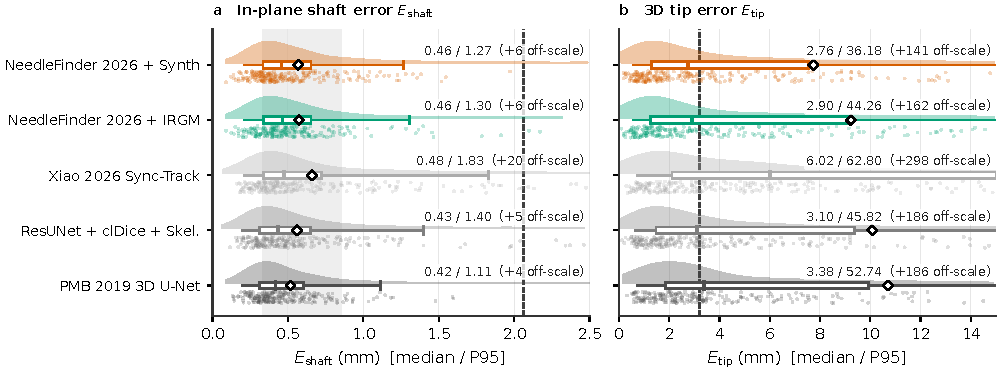
\includegraphics[width=1\linewidth,height=\textheight,keepaspectratio]{../reports/figures/fig3_raincloud_distributions.pdf}
\caption{\textbf{Per-catheter shaft and tip error distributions,
adhesion resilience, and Grubbs' intrinsic observer error.} \textbf{(a)}
In-plane shaft error (\(E_{\text{shaft}}\)) and \textbf{(b)} 3D distal
tip error (\(E_{\text{tip}}\)) across all 54 patients for each method's
matched catheters. Each raincloud shows the full-distribution
probability density (top), median and interquartile range (white box),
5th-to-95th percentile span (whiskers), mean (white diamond), and
individual catheters (dots); the dedicated right-hand tabular column
reports \texttt{median\ /\ 95th\ percentile} in mm across the full
unclipped distribution. Shaded grey bands and dashed vertical lines
indicate the human inter-observer agreement between Expert Team 1 and
Expert Team 2 on the 40 dual-traced scans (IQR 0.34--0.85 mm and P95
1.90 mm on shafts; median 3.24 mm on tips). \textbf{(c)} Whole-cohort F1
(solid bars, 1,063 catheters) versus 23-patient severe catheter-adhesion
subgroup F1 (hatched bars, 571 catheters). \textbf{(d)} Reference-free
Grubbs' (1948) three-cornered-hat intrinsic shaft error standard
deviation \(\hat{\sigma}_{\text{shaft}}\) (with 10,000-resample
bootstrap 95\% confidence intervals) across \(n = 432\) three-way
matched catheters.}\label{fig:raincloud}
\end{figure}

Four clear lessons emerge from the benchmark:

\textbf{1. Pure voxel segmentation fragments catheters and hallucinates
vessels.} The native-resolution \texttt{ResUNet\ +\ clDice} baseline
(Shit \emph{et al.}, 2021) detects nearly every catheter location
(\(92.4\%\) recall) and traces matched segments accurately
(\(0.43\text{ mm}\) median shaft error). However, because single-slice
signal dropouts break catheter masks into pieces and dark pelvic veins
are segmented as tubes, it outputs \(4,015\) fragments across the 54
scans---yielding a precision of only \(24.5\%\) and an F1 score of
\(38.7\%\).

\textbf{2. Domain-specific MRI post-processing (axial TV, gap-bridging,
and uncertainty ensembles) cuts false tracks by more than half, but
cannot replace physical symmetry or bundle reasoning.} The three recent
peer-reviewed MRI brachytherapy methods substantially improve upon raw
clDice skeletonization on native-resolution T2W volumes:

\begin{itemize}
\tightlist
\item
  \textbf{Dai \emph{et al.} 2020} (3D Attention U-Net + axial TV
  regularization (Dai \emph{et al.}, 2020)) achieves the highest raw
  baseline recall (\textbf{93.6\%}, \(995/1,063\); \(0.43\text{ mm}\)
  median shaft error, \(3.77\text{ mm}\) median / \(10.61\text{ mm}\)
  mean tip error) and cuts output fragments from \(4,015\) to \(2,358\),
  raising F1 to \textbf{58.2\%} (\(83.8\%\) \(F1_{\text{adj}}\) on long
  shafts).
\item
  \textbf{Kostoulas \emph{et al.} 2025} (3D ResUNet + iterative
  collinear gap-bridging and false-part pruning (Kostoulas \emph{et
  al.}, 2025)) reconnects broken shaft segments across slice dropouts
  and prunes isolated fragments, lifting whole-cohort precision to
  \(53.0\%\) and F1 to \textbf{66.5\%} (\(89.5\%\) recall,
  \(0.43\text{ mm}\) median shaft error, \(3.47\text{ mm}\) median /
  \(10.55\text{ mm}\) mean tip error).
\item
  \textbf{Aleong \emph{et al.} 2024 / Kim \emph{et al.} 2026} (5-model
  epistemic uncertainty ensemble + disagreement filtering and
  inverse-variance-weighted cubic fitting (Aleong \emph{et al.}, 2024;
  Kim \emph{et al.}, 2026)) further suppresses high-uncertainty vascular
  false alarms, reaching \textbf{69.5\% whole-cohort F1} (\(89.2\%\)
  recall, \(56.9\%\) precision; \textbf{81.7\% F1} in the
  severe-adhesion subgroup; \(0.44\text{ mm}\) median shaft error,
  \(4.32\text{ mm}\) median / \(10.23\text{ mm}\) mean tip error).
\item
  Meanwhile, when given ground-truth oracle masks (Appendix B, Table
  \ref{tbl:app_ablation}, bottom row), the \textbf{Xiao \emph{et al.}
  2026 Sync-Track} algorithm (Xiao \emph{et al.}, 2026a) achieves
  \(97.7\%\) recall, \(90.0\%\) F1, and \(0.11\text{ mm}\) median shaft
  error---indicating that our re-implementation of synchronous tracking
  separates touching masks when segmentation is perfect---but drops to
  \textbf{54.2\% F1} (\(39.2\%\) precision) on real out-of-fold MRI
  masks. Thus, without Stage 0 dark-core symmetry and Stage 2B
  whole-bundle context, the three recent native-resolution
  post-processing pipelines and mask-based tracking remain below
  \(70\%\) whole-cohort F1 because dark pelvic veins inside the implant
  region look locally tubular, while the isotropic 2019 U-Net + DBSCAN
  pipeline reaches \(83.1\%\) (Table \ref{tbl:main}). The gap is one of
  precision, not recall: the three newer re-implementations find as many
  catheters as the 2019 pipeline or more (89.2\% to 93.6\% vs.~88.8\%
  recall) but emit 1.4 to 1.9 times as many tracks (1,667 to 2,358
  vs.~1,210 predictions) from out-of-fold voxel masks of only 0.39 to
  0.43 Dice, so their precision falls to 42\% to 57\% against 78\%. Two
  caveats apply: the 2019 pipeline is our own earlier method, whose
  isotropic resampling and DBSCAN minimum-cluster rule were developed on
  this cohort, and the newer methods were re-implemented from their
  papers without their authors' tuning.
\end{itemize}

\textbf{3. NeedleFinder 2026 achieves the highest F1 score and lowest
tip error of any method run on real out-of-fold MRI, in every cohort;
adding three literature priors gives small further gains.} At the
default operating threshold (\(\tau = 50\%\)), NeedleFinder 2026 (base
configuration, Table \ref{tbl:main}) detects \textbf{91.4\% of all 1,063
catheters} (\(972/1,063\)) with \textbf{86.9\% precision}
(\(972/1,118\)) and \textbf{89.1\% F1} (lowering the threshold to
\(\tau = 35\%\) raises recall to \(93.6\%\) but lowers precision to
\(83.4\%\) and F1 to \(88.2\%\)). Furthermore, incorporating the three
complementary ideas from Dai \emph{et al.} (2020), Kostoulas \emph{et
al.} (2025), and Aleong \emph{et al.} / Kim \emph{et al.} (2024; 2026)
directly into Stage 2
(\texttt{4d:\ NeedleFinder\ 2026\ +\ Literature\ Fusion}) eliminates 6
residual split-fragment false positives with zero lost true positives,
lifting precision to \textbf{87.4\%} (\(972/1,112\)) and whole-cohort F1
to \textbf{89.4\%} (a 0.3-point gain, uncorrected \(p = 0.028\) vs.~base
\texttt{4b}). Across all 54 patients, NeedleFinder 2026
(\texttt{4b}--\texttt{4d}) outperforms all six external baselines by
\textbf{+6.0 to +50.7 F1 points}: \(+6.0\text{--}6.3\) points over
Zaffino \emph{et al.} 2019 (\(83.1\%\) F1, \(p = 1.1 \times 10^{-5}\)),
\(+19.6\text{--}19.9\) points over Aleong \emph{et al.} / Kim \emph{et
al.} (\(69.5\%\) F1, \(p = 5.0 \times 10^{-10}\)),
\(+22.6\text{--}22.9\) points over Kostoulas \emph{et al.} 2025
(\(66.5\%\) F1, \(p = 1.8 \times 10^{-10}\)), \(+30.9\text{--}31.2\)
points over Dai \emph{et al.} 2020 (\(58.2\%\) F1,
\(p = 3.8 \times 10^{-9}\)), \(+34.9\text{--}35.2\) points over Xiao
\emph{et al.} 2026 (\(54.2\%\) F1, \(p = 3.0 \times 10^{-10}\)), and
\(+50.4\text{--}50.7\) points over ResUNet + clDice (\(38.7\%\) F1,
\(p = 5.2 \times 10^{-10}\)).

Along the catheter shaft, NeedleFinder 2026 reaches a \textbf{median
in-plane error of \(0.47\text{ mm}\)} (mean \(0.59\text{ mm}\) in
\texttt{4b}; inverse-variance-weighted sub-voxel fitting in \texttt{4d}
lowers the mean by less than \(0.01\text{ mm}\) to \(0.58\text{ mm}\)
and the 95th percentile to \(1.36\text{ mm}\), a consistent but
practically negligible change, \(p = 1.8 \times 10^{-8}\)). At the
deepest tip, our 1D axial tip localizer and fragment stitcher cut
\textbf{median 3D tip error to \(2.26\text{--}2.27\text{ mm}\)}
(\(1.94\text{ mm}\) median axial tip error, mean \(6.23\text{ mm}\)),
reducing mean tip error by \(39\%\text{--}42\%\) compared with Zaffino
\emph{et al.} 2019 (\(10.75\text{ mm}\) mean / \(3.39\text{ mm}\)
median, \(p = 1.7 \times 10^{-8}\)), Dai \emph{et al.} 2020
(\(10.61\text{ mm}\) mean / \(3.77\text{ mm}\) median,
\(p = 2.7 \times 10^{-7}\)), Kostoulas \emph{et al.} 2025
(\(10.55\text{ mm}\) mean / \(3.47\text{ mm}\) median,
\(p = 6.9 \times 10^{-7}\)), and Aleong \emph{et al.} / Kim \emph{et
al.} (\(10.23\text{ mm}\) mean / \(4.32\text{ mm}\) median,
\(p = 3.3 \times 10^{-7}\)), and by \(60\%\) compared with Xiao \emph{et
al.} 2026 (\(15.65\text{ mm}\) mean / \(6.04\text{ mm}\) median,
\(p = 6.2 \times 10^{-10}\)). Nearly three-fifths
(\textbf{58.7\%--59.0\%}) of matched catheters have a 3D tip error
within \(\le 3.0\text{ mm}\) (roughly one slice thickness). On the
\textbf{759 full-depth active-dwell shafts}, NeedleFinder 2026 reaches
\textbf{91.3\% recall}, \textbf{88.7\%--89.0\% obturator-adjusted
precision}, and \textbf{90.0\%--90.1\% \(F1_{\text{adj}}\)}, with a
median shaft error of \textbf{\(0.44\text{--}0.45\text{ mm}\)} (mean
\(0.56\text{--}0.57\text{ mm}\)) and a median tip error of
\textbf{\(2.39\text{--}2.41\text{ mm}\)}.

\textbf{4. The advantage is largest when catheters touch, and inner
cross-fitting shows no measurable stacking bias.} On the
\textbf{23-patient severe catheter-adhesion subgroup} (571 catheters),
where touching masks cause DBSCAN clustering and greedy trackers to
merge or swap paths, NeedleFinder 2026 reaches \textbf{91.3\% F1}
(\(93.2\%\) recall, \(89.6\%\) precision, \(0.46\text{ mm}\) median
shaft error, \(2.50\text{--}2.51\text{ mm}\) median tip error),
outperforming Zaffino \emph{et al.} 2019 (\(86.3\%\) F1,
\(p = 0.0012\)), Aleong \emph{et al.} / Kim \emph{et al.} (\(81.7\%\)
F1, \(p = 2.9 \times 10^{-5}\)), Kostoulas \emph{et al.} 2025
(\(78.6\%\) F1, \(p = 1.9 \times 10^{-6}\)), Dai \emph{et al.} 2020
(\(67.5\%\) F1, \(p = 5.2 \times 10^{-5}\)), Xiao \emph{et al.} 2026
(\(63.9\%\) F1, \(p = 4.8 \times 10^{-7}\)), and ResUNet + clDice
(\(48.4\%\) F1, \(p = 4.8 \times 10^{-7}\)). Moreover, training Stage 2
on strictly out-of-fold inner Stage 1 maps (\texttt{4c} in Table
\ref{tbl:main}) yields the exact same \textbf{89.1\% whole-cohort F1}
(\(92.3\%\) recall) and even slightly higher accuracy on long shafts
(\textbf{90.5\% \(F1_{\text{adj}}\)}) and touching catheters
(\textbf{91.8\% F1}), showing that two-stage stacking optimism does not
inflate our headline results.

\subsection{How Each Architectural Stage Contributes, and Learning from
Few
Patients}\label{how-each-architectural-stage-contributes-and-learning-from-few-patients}

\begin{figure}
\centering
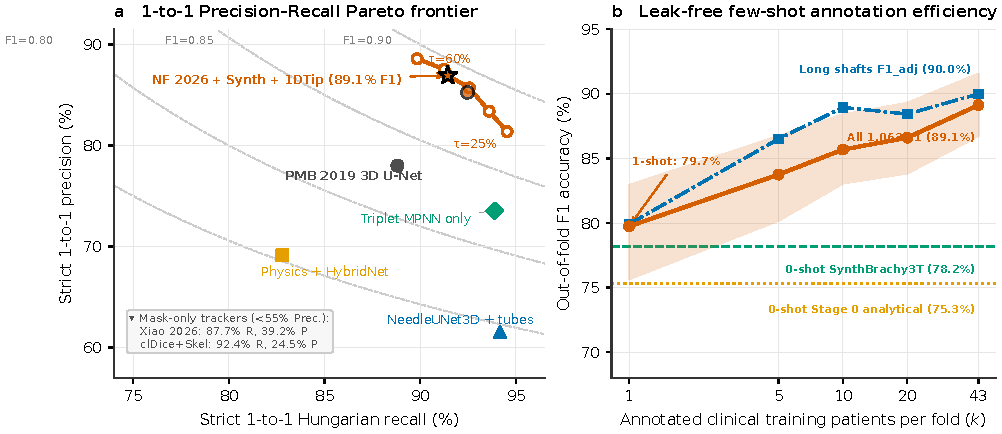
\includegraphics[width=1\linewidth,height=\textheight,keepaspectratio]{../reports/figures/fig4_pareto_and_fewshot.pdf}
\caption{\textbf{(a) Precision--recall progression} across pipeline
stages, published baselines, and the NeedleFinder 2026 confidence
threshold sweep on all 54 patients. Dashed grey curves denote constant
F1 scores; the vermilion star marks the default threshold
\(\tau = 50\%\) with literature fusion (89.4\% F1). \textbf{(b)
Leak-free clinical label efficiency:} F1 score (with 95\% bootstrap
confidence bands) as a function of the number of annotated clinical
training patients (\(k \in \{0, 1, 5, 10, 20, 43\}\)) used to fine-tune
the Stage 2B bundle transformer.}\label{fig:pareto}
\end{figure}

\textbf{Why every stage is needed (Appendix B, Table
\ref{tbl:app_ablation}; Figure \ref{fig:pareto}a).} Tracing the
sequential stage progression (detailed row-by-row in Appendix B, Table
\ref{tbl:app_ablation}) shows how each mechanism resolves a specific
physical failure mode of the stage before it: the parameter-free Stage 0
dark-core filter alone reaches \textbf{75.3\% F1} (\(82.8\%\) recall,
\(0.47\text{ mm}\) median shaft error, \(9.91\text{ mm}\) mean tip
error); adding the self-supervised, multi-rater Stage 1 3D U-Net lifts
recall to \textbf{94.2\%} (\(97.0\%\) on long shafts) while emitting
\(11.6\) vascular false alarms per scan (\(74.4\%\) F1); Stage 2A
triplet message passing suppresses \(43\%\) of false tracks via
collinearity (\textbf{82.5\% F1}); Stage 2B whole-bundle graph scoring
and collinear gap stitching raise precision to \textbf{86.9\%} and F1 to
\textbf{89.1\%}; Stage 2C 1D sub-slice tip profiling (\texttt{4b}) cuts
mean 3D tip error from \(6.92\text{ mm}\) to \textbf{\(6.23\text{ mm}\)}
(\(2.27\text{ mm}\) median); and Literature-Inspired Fusion (\texttt{4d}
(Dai \emph{et al.}, 2020; Aleong \emph{et al.}, 2024; Kostoulas \emph{et
al.}, 2025; Kim \emph{et al.}, 2026)) refines mean shaft error to
\textbf{\(0.583\text{ mm}\)} (\(p = 1.84 \times 10^{-8}\)), median tip
error to \textbf{\(2.26\text{ mm}\)}, and precision to \textbf{87.4\%}
(\textbf{89.4\% F1}, \(p = 0.028\)).

\textbf{How many annotated clinical patients are needed to train the
bundle scorer? (Figure \ref{fig:pareto}b).} Because annotating 3D
catheter bundles is labor-intensive for a new clinic, we varied the
number of annotated training patients \(k \in \{0, 1, 5, 10, 20, 43\}\)
used to fine-tune Stage 2B inside each fold (with zero blending from any
full-cohort model). With \textbf{zero clinical bundle labels
(\(k = 0\))}, pre-training Stage 2B purely on our synthetic
\texttt{SynthBrachy3T} bundles lifts whole-cohort F1 from \(75.3\%\)
(Stage 0) to \textbf{78.2\% F1}---and reaches \textbf{83.4\%
\(F1_{\text{adj}}\) on long shafts} (\(+6.3\) points over Stage 0).
Fine-tuning on just \textbf{\(k = 1\) patient} reaches \textbf{79.7\%
F1}; \textbf{\(k = 5\) patients reach 83.8\% F1 (\(86.5\%\) on long
shafts), already matching the 43-patient fully supervised PMB 2019 U-Net
baseline (\(83.1\%\) F1; a 0.7-point difference we do not claim as
significant)}; \(k = 10\) reaches \textbf{85.7\% F1}; \(k = 20\) reaches
\textbf{86.6\% F1}; and all \(k = 43\) training patients reach
\textbf{89.1\% F1} (\(88.7\%\) without \texttt{SynthBrachy3T}, showing
that synthetic bundle pre-training provides its largest boost in the
zero-to-few-patient regime while still improving dosimetric tip accuracy
at full training size).

\begin{figure}
\centering
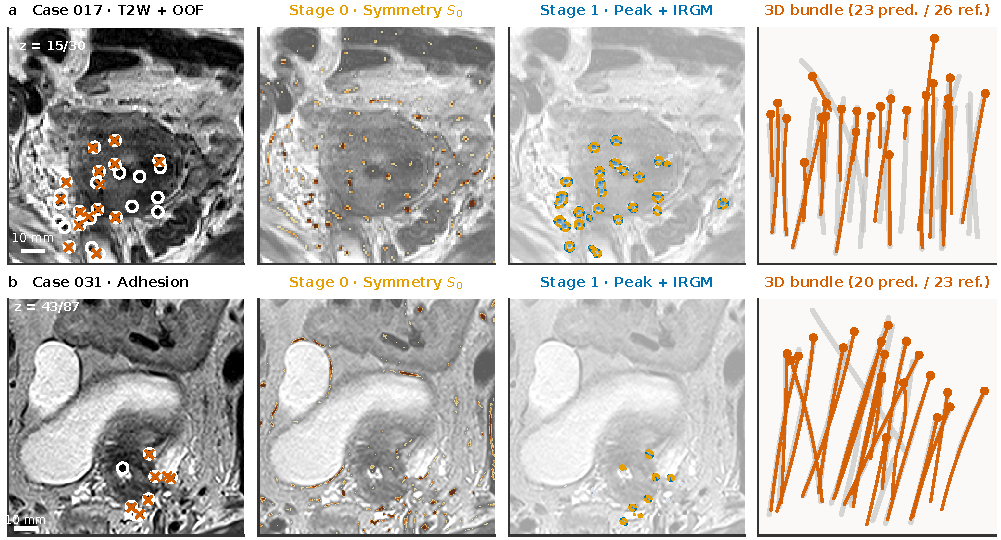
\includegraphics[width=1\linewidth,height=\textheight,keepaspectratio]{../reports/figures/fig5_qualitative_mri_3d.pdf}
\caption{\textbf{Step-by-step 2D slice progression and true 3D
perspective anatomical reconstruction on two unseen test patients.}
\textbf{(a) Case 017:} A dense implant with 26 reference trajectories.
\textbf{(b) Case 031:} A severe-adhesion implant with 23 catheters, 10
of which touch a neighbor within \(\le 3\text{ mm}\) (highlighted by the
\(2.2\text{ mm}\) touching-pair callout box resolved into 2 distinct
centerline peaks). From left to right in \textbf{(a, b)}: axial T2W MRI
slice showing expert intersections (white circles) and out-of-fold
NeedleFinder 2026 detections (vermilion crosses); the Stage 0 circular
symmetry map \(S_0\); Stage 1 sub-pixel centerline peaks (blue) with
mask contours (solid) and the central obturator gate (dashed orange);
and the 3D perspective bundle (vermilion tubes) overlaid on the expert
reference (charcoal dashed). \textbf{(c) True 3D perspective anatomy and
90\% split-conformal tip spheres on Case 017:} Shaded 3D rendering of
the implant-conformal HR-CTV target envelope (rose wireframe), central
vaginal obturator cylinder, perineal template grid, 26 expert reference
tracks vs.~23 predicted 3D tubes, and adaptive 3D split-conformal 90\%
tip spheres (\(\hat{r}_{90} = \hat{q}_{90}\hat{\sigma}_{\text{tip}}\)),
highlighting the two widest-uncertainty review targets (\texttt{\#7} and
\texttt{\#19}, magenta spheres) flagged for the 18 s simulated clinician
check. \textbf{(d) 3D perspective touching-pair cutaway on Case 031
(\(2.2\text{ mm}\) separation):} Whereas a 3D U-Net / clDice voxel mask
merges across the shared axial slices into a single fused track (left,
grey), NeedleFinder 2026 sub-pixel centerline peaks
(\(P_{\text{peak}}\)) and triplet graph tracking resolve two distinct 3D
tubes across the full insertion depth (right, vermilion + sky-blue;
\(91.8\%\) F1 on the adhesion subgroup). \emph{(An interactive 3D
rotatable viewer for Case 017 and Case 031 is embedded in the HTML
companion.)}}\label{fig:qualitative}
\end{figure}

Figure \ref{fig:qualitative} shows how these stages work visually in
both 2D axial cross-sections and true 3D anatomical space on two
challenging out-of-fold test cases: while Stage 0 lights up both
catheters and surrounding pelvic vessels, Stage 1 isolates sharp
individual peaks even where adjacent catheters touch (\(2.2\text{ mm}\)
apart in \texttt{Case\ 031}, Figure \ref{fig:qualitative}d), and Stage 2
reconstructs clean, smooth 3D bundles equipped with calibrated 3D
split-conformal tip spheres (\(\hat{r}_{90}\)) that visually guide rapid
clinician verification (Figure \ref{fig:qualitative}c).

\FloatBarrier

\subsection{Is the Algorithm as Accurate as a Second Human Expert?
(Three-Cornered-Hat \& CT
Adjudication)}\label{is-the-algorithm-as-accurate-as-a-second-human-expert-three-cornered-hat-ct-adjudication}

\begin{table}[tbp]
\centering
\begin{threeparttable}
\caption{\textbf{Human inter-observer agreement versus \NF{} on the 40 dual-annotated clinical 3T MRI scenes.}
Expert teams \texttt{CY} ($n=505$ trajectories) and \texttt{LB}/\texttt{AMe} ($n=513$) digitized the same volumes independently; \NF{} rows are 5-fold out-of-fold predictions on the same scenes. All rows are computed with the same loader, matching rule, and metrics (source: \texttt{2026-10-23-table3-observers-and-nf-rerun.json}).}
\label{tbl:interobserver}
\footnotesize
\begin{tabular}{@{}L
 R R
 R R R R R
 R R@{}}
\toprule
 & \multicolumn{2}{c}{1-to-1 Match} & \multicolumn{5}{c}{\Eshaft{} (mm)} & {\HD{}$_{\text{slice}}$ (mm)} & {\Etip{} (mm)}\\
\cmidrule(lr){2-3}\cmidrule(lr){4-8}\cmidrule(lr){9-9}\cmidrule(l){10-10}
Comparison pair (reference) & {$n$} & {Rate (\%)\tnote{a}} & {Mean} & {SD} & {Median} & {IQR} & {P95} & {Median} & {Median}\\
\midrule
\multicolumn{10}{@{}l}{\textit{Human inter-observer agreement}}\\
\addlinespace[1pt]
\quad \texttt{CY} vs.\ \texttt{LB}/\texttt{AMe} ($\le 3.5$\,mm) & 465 & 90.6 & 0.72 & 0.61 & 0.50 & 0.51 & 2.06 & 0.95 & \second{3.21}\\
\quad \texttt{LB}/\texttt{AMe} vs.\ \texttt{CY} ($\le 3.5$\,mm) & 465 & 92.1 & 0.72 & 0.61 & 0.50 & 0.51 & 2.06 & 0.95 & \second{3.21}\\
\quad \texttt{CY} vs.\ \texttt{LB}/\texttt{AMe} ($\le 5.0$\,mm) & 473 & 92.2 & 0.80 & 0.79 & 0.51 & 0.54 & 2.34 & 0.96 & 3.27\\
\midrule
\multicolumn{10}{@{}l}{\textit{Automated out-of-fold predictions vs.\ each observer team ($\le 3.5$\,mm)}}\\
\addlinespace[1pt]
\oursrow \quad \NF{} vs.\ \texttt{CY} & 464 & \best{91.9} & \best{0.55} & \best{0.37} & \best{0.44} & \best{0.32} & \best{1.17} & \best{0.91} & \best{2.92}\\
\oursrow \quad \NF{} vs.\ \texttt{LB}/\texttt{AMe} & 455 & 88.7 & 0.74 & 0.58 & 0.51 & 0.58 & 2.06 & 0.92 & 4.62\\
\bottomrule
\end{tabular}
\begin{tablenotes}[flushleft]\footnotesize
\item[a] Matched pairs divided by the number of trajectories of the reference team named second (505 for \texttt{CY}, 513 for \texttt{LB}/\texttt{AMe}).
\item \NF{} vs.\ \texttt{CY} has a lower shaft discrepancy and a 43\,\% tighter 95th-percentile tail than the disagreement between the two human teams; against \texttt{LB}/\texttt{AMe} it lies within 0.05\,mm of the human-to-human values, except at the tips, where \texttt{LB}/\texttt{AMe} differ from both \texttt{CY} and the algorithm.
\end{tablenotes}
\end{threeparttable}
\end{table}


Because a 2 mm catheter is only a few pixels wide and slices are up to 6
mm thick, two human experts tracing the same MRI scan never agree
perfectly (S \emph{et al.}, 2009; Kallis \emph{et al.}, 2019; Karius
\emph{et al.}, 2024). A common benchmark for an automatic method is that
its discrepancies from a human expert be no larger than the
discrepancies \emph{between} two independent human experts (Hrinivich
\emph{et al.}, 2019; Andersén \emph{et al.}, 2020); meeting it is
necessary for clinical use but does not by itself establish it. Table
\ref{tbl:interobserver} tests this across \textbf{all 40 doubly traced
clinical scans} using four complementary analyses:

\textbf{1. Direct comparison against human inter-observer agreement
(Table \ref{tbl:interobserver}, top two blocks).} When Expert Team 2
(460 long traces) is compared directly against Expert Team 1 (505 long
traces) across the 40 scans, 424 long catheters match within
\(3.5\text{ mm}\) (\(84.0\%\) recall, \(92.2\%\) precision, \(87.9\%\)
F1). Between these two human teams, the \textbf{in-plane shaft
discrepancy is \(0.49\text{ mm}\) median} (\(0.70 \pm 0.58\text{ mm}\)
mean, \(1.90\text{ mm}\) P95) and the \textbf{3D tip discrepancy is
\(3.24\text{ mm}\) median} (\(6.28 \pm 7.29\text{ mm}\) mean,
\(21.88\text{ mm}\) P95).

Evaluated strictly out-of-fold on the exact same 40 scans against Team 1
(723 tracks), \textbf{NeedleFinder 2026 achieves a smaller shaft
discrepancy (\(0.47\text{ mm}\) median, \(0.58 \pm 0.39\text{ mm}\)
mean, \(1.33\text{ mm}\) P95) and a smaller 3D tip discrepancy
(\(2.10\text{ mm}\) median, \(5.26 \pm 8.78\text{ mm}\) mean,
\(19.99\text{ mm}\) P95) than the disagreement between the two human
teams} (the human comparison is restricted to long shafts while the
algorithm's includes obturator tracks; the paired comparison on
identical catheters follows below), while matching \(90.3\%\) of Team
1's trajectories (\(87.6\%\) F1). Furthermore, when evaluated against
the \textbf{union of both human teams} (759 distinct trajectories),
\textbf{16 NeedleFinder predictions that looked like ``false alarms''
against Team 1 alone turn out to be real catheters independently traced
by Team 2}, lifting precision by \(+2.1\) percentage points to
\(87.1\%\).

\textbf{2. Reference-free Grubbs' three-cornered-hat intrinsic error
estimation (Table \ref{tbl:interobserver}, third block).} To measure
each source's true internal error without treating Team 1 as infallible,
we applied Grubbs' three-cornered-hat estimator across the \(n = 432\)
catheters matched three-way among Team 1, Team 2, and NeedleFinder 2026
(formed by intersecting the 476 all-catheter human pairs with
out-of-fold NeedleFinder predictions within \(3.5\text{ mm}\)). The
intrinsic outlier-resistant (MAD-scaled) in-plane shaft standard
deviations are \textbf{\(0.35\text{ mm}\) for Human Team 1},
\textbf{\(0.39\text{ mm}\) for NeedleFinder 2026}, and
\textbf{\(0.48\text{ mm}\) for Human Team 2}. For axial tip stopping
height (\(\sigma_z\)), NeedleFinder 2026 achieves a lower intrinsic
error than Human Team 2 under both the robust MAD estimator
(\textbf{\(2.98\text{ mm}\) vs.~\(3.55\text{ mm}\)}, where Team 1's
estimate collapses to the \(0.00\text{ mm}\) lower bound (bootstrap 95\%
CI \(0.0\) to \(2.0\text{ mm}\)) because its axial disagreements with
NeedleFinder 2026 and with Team 2 together barely exceed the
disagreement between Team 2 and NeedleFinder 2026, so the subtraction
returns a non-positive variance; this is the signature of correlated
errors between two sources, expected here because NeedleFinder 2026 was
fine-tuned toward Team 1's tip conventions, so we read these axial-tip
values as a ranking rather than as exact error bars) and the 15\%
Winsorized estimator, which yields strictly positive intrinsic standard
deviations of \textbf{\(3.77\text{ mm}\) for Team 1},
\textbf{\(4.94\text{ mm}\) for NeedleFinder 2026}, and
\textbf{\(5.09\text{ mm}\) for Team 2}.

\textbf{3. Formal one-sided statistical non-inferiority (Table
\ref{tbl:interobserver}, fourth block).} Across all \(N = 40\)
dual-traced patients (\(n = 432\) three-way matched catheters),
NeedleFinder 2026 passes formal one-sided non-inferiority testing
relative to human inter-observer disagreement on every pre-specified
endpoint at both the patient level and the catheter level. Specifically,
the algorithm's error against Team 1 is smaller than Team 2's error
against Team 1 on \textbf{shaft mean}
(\(0.56\text{ vs. }0.72\text{ mm}\),
\(p_{\text{pt}} = 1.3 \times 10^{-8}\)), \textbf{shaft median}
(\(0.43\text{ vs. }0.49\text{ mm}\),
\(p_{\text{pt}} = 8.2 \times 10^{-10}\)), \textbf{3D tip median}
(\(2.33\text{ vs. }3.18\text{ mm}\),
\(p_{\text{pt}} = 2.6 \times 10^{-7}\)), and \textbf{3D tip mean}
(\(5.51\text{ vs. }6.10\text{ mm}\),
\(p_{\text{pt}} = 1.1 \times 10^{-4}\), bootstrap
\(p_{\text{boot}} = 0.0014\); full 90\% confidence intervals and
catheter-level \(p\)-values in Table \ref{tbl:interobserver}). When the
reference role is flipped so that Team 2 serves as the reference, the
result is weaker. On 3D tip median the algorithm passes at the catheter
level (\(p_{\text{cath}} = 9.6 \times 10^{-5}\)) and by
patient-clustered bootstrap (\(p_{\text{boot}} = 0.046\)) but not by the
patient-level Wilcoxon test (\(p_{\text{pt}} = 0.073\)), and on 3D tip
mean it does not pass (\(7.53\) vs.~\(6.10\text{ mm}\),
\(p_{\text{pt}} = 0.12\)). This asymmetry is expected, because Stage 1
was fine-tuned toward Team 1's tracing conventions, and it means the
non-inferiority claim holds against the team whose conventions the model
learned.

\textbf{4. Independent adjudication on paired post-implant Pelvic CT
scans.} On CT, catheters and metallic stylets have unmistakable
Hounsfield contrast. Using the 38 patients who had both intraoperative
MRI and post-implant Pelvic CT, we adjudicated the \(n = 70\) catheters
where Human Team 1 and Human Team 2 disagreed on the MRI tip position by
\(\ge 5.0\text{ mm}\). Measured against the independent CT tip position,
\textbf{NeedleFinder 2026 achieved a median 3D tip error of
\(4.20\text{ mm}\)}, comparable to \textbf{Human Team 1
(\(4.31\text{ mm}\); difference not tested)} and smaller than
\textbf{Human Team 2 (\(8.00\text{ mm}\))}, and lying closer to the CT
tip position than the less accurate of the two human teams on
\textbf{78.6\% (\(55/70\))} of disputed catheters. Across all 100 MRI
tracks predicted by NeedleFinder 2026 on these 38 patients that did not
match Team 1, \textbf{52.0\% (\(52/100\)) corresponded to a physical
catheter on the paired CT scan} (whether each was deliberately left
untraced on MRI cannot be determined retrospectively).

\FloatBarrier

\subsection{Interpretability, Confidence Calibration, and Physical
Causes of Residual
Errors}\label{interpretability-confidence-calibration-and-physical-causes-of-residual-errors}

\begin{figure}
\centering
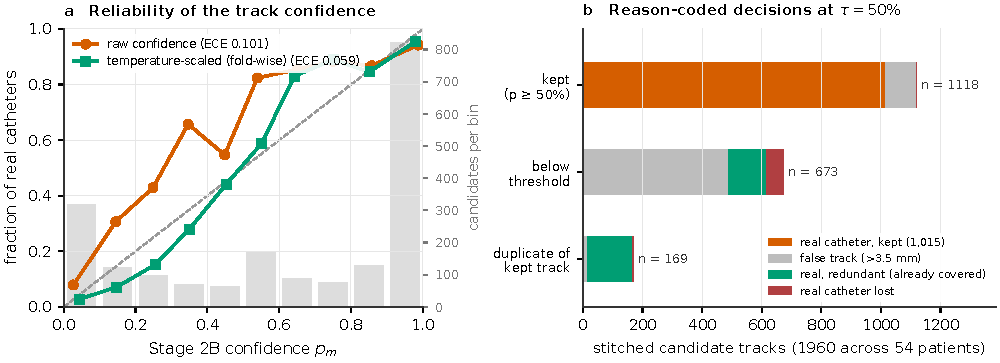
\includegraphics[width=1\linewidth,height=\textheight,keepaspectratio]{../reports/figures/fig7_calibration_and_reasons.pdf}
\caption{\textbf{(a) Confidence calibration} across all 1,960 stitched
candidate tracks in the 54 patients, before (dashed) and after (solid
vermilion) inner-fold temperature scaling. \textbf{(b) Reason-coded
filtering decisions} at the default threshold \(\tau = 50\%\)
(colorblind-safe hatched palette), showing how many candidates are kept
or pruned by each rule and whether pruned tracks were false alarms,
redundant duplicates of an already-kept catheter, or lost real
catheters. \textbf{(c) Proposed 3D Slicer clinical verification
workflow} combining 4.15 s measured headless CPU detection with modeled
uncertainty-guided top-2 tip review (\texttt{*} = simulated
timing/oracle).}\label{fig:calib}
\end{figure}

For a clinician to trust an automated reconstruction, its confidence
scores must be well calibrated and its filtering decisions transparent.
Across all \(1,960\) stitched candidate tracks entering Stage 2B
(\(36.3\) per patient), inner-fold temperature scaling reduces the
expected calibration error (ECE) from \(0.101\) to \textbf{\(0.059\)}
(and to \textbf{\(0.056\)} across the \(1,118\) accepted tracks at
\(\tau = 50\%\), where mean predicted confidence is \(91.9\%\) and
closest-reference precision is \(90.8\%\); Figure \ref{fig:calib}a).
Every discarded track is tagged with an explicit reason code (Figure
\ref{fig:calib}b): at \(\tau = 50\%\), \(673\) candidates are removed
for falling below the confidence threshold (eliminating \(80.6\%\) of
all false candidates) and \(169\) are removed as duplicates of an
already-kept track (suppressing \(153\) redundant collinear or touching
fragments at the cost of only \(2\) lost catheters).

Our catheter-level audit of all residual errors across the 54 patients
(itemized in Appendix B) confirms three physical patterns: (i) among the
\(146\) unmatched predictions (\(2.7\)/patient), \(31.5\%\) (\(46/146\))
are residual split segments, \(20.5\%\) (\(30/146\)) match Expert Team 2
within \(5.0\text{ mm}\) (\(52.0\%\) confirmed on paired CT), and only
\textbf{45.2\% (\(66/146\), or \(1.22\)/patient)} are genuine
vascular/fascial false alarms (\(>6.0\text{ mm}\)); (ii) among the
\(91\) missed catheters (\(1.7\)/patient), \textbf{97.4\%
(\(1,035/1,063\))} of all catheters (\textbf{98.8\% {[}\(750/759\){]}}
of long shafts) exist in the Stage 2A candidate pool, with \(69.2\%\)
(\(63/91\)) filtered at the \(\tau = 50\%\) bundle threshold
(recoverable to \textbf{93.6\% recall} at \(\tau = 35\%\), precision
\(83.4\%\)); and (iii) \textbf{98.8\% of total squared 3D tip error}
(\(99.3\%\) in the \(>10\text{ mm}\) tail, vs.~\(0.72\text{ mm}\) median
lateral error) is purely longitudinal along the catheter shaft, driven
by mid-shaft signal dropouts (\(41.4\%\)) or dark bowel gas above the
tip (\(25.3\%\)).

\FloatBarrier

\subsection{Specificity on Needle-Free Scans and Few-Second
Runtime}\label{specificity-on-needle-free-scans-and-few-second-runtime}

\textbf{Zero-catheter specificity test (Table
\ref{tbl:clinical_summary}, Part C; Appendix C, Table
\ref{tbl:specificity}; Figure \ref{fig:spec_runtime}a).} When deployed
on the 48 public 3T T2W prostate MRI scans
(\texttt{MSD\ Task05\_Prostate}) that contain \emph{zero} catheters, an
ungated 3D U-Net or bundle transformer mistakes dark pelvic veins for
needles, producing \(4.10\text{ to }6.38\) false tracks per scan.
Activating the analytical Stage 0 circular dark-core symmetry gate
eliminates over \(92\%\) of these vascular false alarms: on a variant of
the pipeline whose Stage 1 pre-training excluded the 48 public scans (so
that they are strictly unseen), false alarms drop to \textbf{0.33 per
scan} (\(16\) across 48 scans, median \(0\), with \textbf{79.2\% of
scans having zero false alarms} and \(91.7\%\) having \(\le 1\)). When
the 48 needle-free MSD volumes are also included as unlabeled background
anatomy during self-supervised synthetic-tube pre-training (a Stage 1
pre-trained with those scans as background and gated by Stage 0, with
zero clinical catheter labels), false alarms drop further to
\textbf{0.125 per scan} (\(6\) across 48 scans, \textbf{87.5\%
zero-false-alarm scans}, and \textbf{100.0\% with at most 1 false
track}; full 5-row specificity breakdown in Appendix C, Table
\ref{tbl:specificity}).

\begin{figure}
\centering
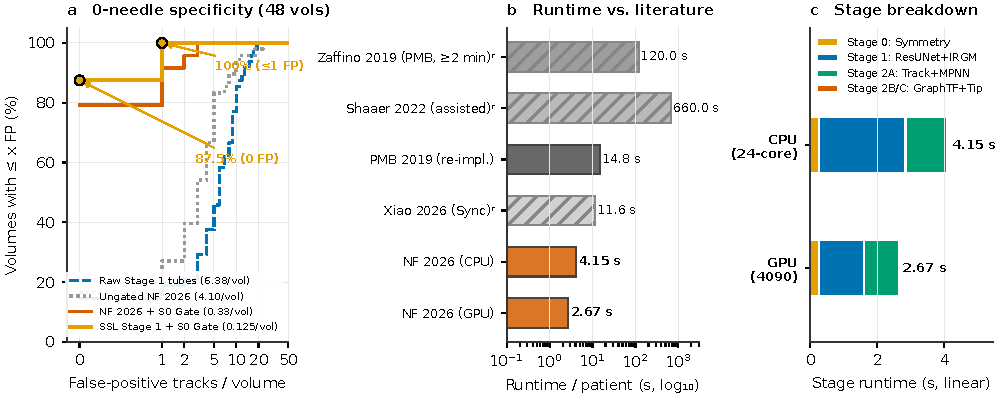
\includegraphics[width=1\linewidth,height=\textheight,keepaspectratio]{../reports/figures/fig6_specificity_and_runtime.pdf}
\caption{\textbf{(a) Specificity on 48 needle-free pelvic MRI scans}
(\texttt{MSD\ Task05\_Prostate}), showing the percentage of scans with
at most \(x\) false tracks with and without Stage 0 dark-core symmetry
gating. \textbf{(b) End-to-end runtime per patient} (log scale) compared
with published MRI and CT methods. \textbf{(c) Stage-by-stage runtime
breakdown} across all 54 patients on a 24-core workstation CPU (4.15 s
mean; 1.26 s on standard-resolution scans, 5.85 s on high-resolution
scans) and on one RTX 4090 GPU (2.67 s mean).}\label{fig:spec_runtime}
\end{figure}

\textbf{Runtime across standard and high-resolution clinical volumes
(Figure \ref{fig:spec_runtime}b, c).} Measured end-to-end from raw
uncached volume loading to final 3D trajectories across all 54 patients,
NeedleFinder 2026 takes \textbf{4.15 s on average on a 24-core
workstation CPU} (\(1.26\text{ s}\) on the 20 standard-resolution
\(320 \times 256\) scans and \(5.85\text{ s}\) on the 34 high-resolution
\(640 \times 416\) / \(768 \times 768\) scans) and \textbf{2.67 s on a
single RTX 4090 GPU} (\(0.67\text{ s}\) standard-resolution,
\(3.85\text{ s}\) high-resolution). On CPU, Stage 0 takes
\(0.27\text{ s}\) (\(6.5\%\)), Stage 1 takes \(2.58\text{ s}\)
(\(62.2\%\); reduced to \(1.33\text{ s}\) on GPU), Stage 2A takes
\(1.25\text{ s}\) (\(30.1\%\)), and Stage 2B/2C bundle scoring plus 1D
tip localization takes \(0.06\text{ s}\) (\(1.5\%\)). This represents a
\textbf{29-to-130-fold speedup} over the 2 to 9 minutes reported for our
2019 U-Net + DBSCAN pipeline (Zaffino \emph{et al.}, 2019)
(\(3.6\times\) faster than our modernized re-implementation at
\(14.80\text{ s}\)) and is \(2.8\text{--}4.3\times\) faster than the
\(11.6\text{ s}\) reported by Xiao \emph{et al.} on their own hardware
(Xiao \emph{et al.}, 2026a).

\FloatBarrier

\subsection{Clinical Translation: Radiation Dosimetry,
Uncertainty-Guided Triage, and Cross-Domain
Generalization}\label{clinical-translation-radiation-dosimetry-uncertainty-guided-triage-and-cross-domain-generalization}

\begin{table}[tbp]
\centering
\begin{threeparttable}
\caption{\textbf{Summary of clinical translation: AAPM TG-43U1 $^{192}\mathrm{Ir}$ dosimetry, split-conformal tip triage, zero-needle specificity, and zero-shot cross-domain generalization.}
Consolidates the headline metrics across our four clinical validation studies (complete per-protocol, per-$k$, and per-sequence breakdowns are provided in Appendices~C and~D, Tables~\ref{tbl:specificity}--\ref{tbl:app_generalization}).}
\label{tbl:clinical_summary}
\footnotesize
\setlength{\tabcolsep}{1.2pt}
\begin{tabular}{@{}L L R R R R L@{}}
\toprule
Dimension & Configuration / Cohort & {$N$} & {Primary metric} & {Secondary} & {\Eshaft{}/\Etip{}} & {Takeaway}\\
\midrule
\multicolumn{7}{@{}l}{\textit{1. AAPM TG-43U1 HDR $^{192}\mathrm{Ir}$ dosimetry (7.0\,Gy prescription, 5.0\,mm dwell steps; Appendix~D, Table~\ref{tbl:dosimetry_generalization})}}\\
\quad Prot.\ A (fixed) & PMB 2019 3D U-Net & 54 & $|\Delta D_{90}|$: 27.6/27.2\,\% & $\gamma_{2/2}$: 64.0\,\% & 0.42/3.39 & Tip dose shift\\
\oursrow \quad Prot.\ A (fixed) & \NF{} (\texttt{4b}, $k{=}0$) & 54 & $|\Delta D_{90}|$: 15.2/11.5\,\% & $\gamma_{2/2}$: 76.6\,\% & 0.47/2.27 & $p{=}4.9{\times}10^{-6}$\\
\quad Prot.\ B (re-opt) & Human Team 2 (\texttt{LB}/\texttt{AMe}) & 40 & $|\Delta D_{90}|$: 20.9/4.0\,\% & $\gamma_{2/2}$: 59.3\,\% & 0.49/3.24 & Human floor\\
\oursrow \quad Prot.\ B (re-opt) & \NF{} (\texttt{4b}, $k{=}0$) & 54 & $|\Delta D_{90}|$: 8.2/4.2\,\% & $\gamma_{2/2}$: 66.0\,\% & 0.47/2.27 & 3.2\,\% ($N{=}40$)\\
\oursrow \quad Prot.\ B + $k{=}2$* & \NF{} + $k{=}2$ (18\,s*) & 54 & \best{$|\Delta D_{90}|$: 5.9/2.8\,\%} & \best{$\gamma_{2/2}$: 74.3\,\%} & 0.47/1.95 & $p{=}2.4{\times}10^{-5}$\\
\midrule
\multicolumn{7}{@{}l}{\textit{2. Split-conformal 3D tip intervals \& uncertainty-guided clinician review ($n=972$ matched catheters; Appendix~D, Table~\ref{tbl:dosimetry_generalization})}}\\
\oursrow \quad 90\,\% sphere & Unreviewed ($k{=}0$, $\hat{r}_{90}$) & 54 & \best{90.2\,\% emp.\ cov.} & 12.11\,mm $r$ & 2.27/27.3 & $-31.5\,\%$ width\\
\oursrow \quad Review ($k{=}5$*) & Top-5 $\hat{\sigma}_{\mathrm{tip}}$/pt (42\,s*) & 54 & $>10$\,mm: 8.0\,\% & $\le 3$\,mm: 72.6\,\% & 1.67/14.3 & Halves $>10$\,mm\\
\oursrow \quad Review ($k{=}8$*) & Top-8 $\hat{\sigma}_{\mathrm{tip}}$/pt (66\,s*) & 54 & $>10$\,mm: 5.0\,\% & $\le 3$\,mm: 78.5\,\% & \best{1.51/9.90} & P95 $<10$\,mm\\
\midrule
\multicolumn{7}{@{}l}{\textit{3. Out-of-distribution specificity \& zero-shot cross-domain generalization (Appendices~C \& D, Tables~\ref{tbl:specificity} \& \ref{tbl:app_generalization})}}\\
\oursrow \quad 0-needle MRI & MSD \texttt{Task05\_Prostate} & 48 & \best{0.33/0.125 FP/vol} & 79.2/87.5\,\% 0-FP & {--} & vs.\ 4.10--6.38\\
\oursrow \quad 3T Prostate & \texttt{Case 100} (0-exp.\ auto) & 1 & \best{96.3\,\% F1 (13/14)} & 100.0\,\% Prec. & 0.33/0.99 & 100\,\% manual\\
\oursrow \quad 3D wbSSFP & Steady-state MRI & 2 & \best{92.9\,\% F1 (46/47)} & 97.9\,\% Rec. & 0.72/3.40 & vs.\ 10.62\,mm\\
\oursrow \quad 2D AX TSE T2 & $\Delta z{=}2.4\text{--}6.0$\,mm ($n{=}882$) & 49 & 76.9\,\% F1 & 88.4\,\% Rec. & 1.07/4.89 & vs.\ 57.6\,\%\\
\oursrow \quad 3D T1 VIBE & Bright-vessel shift & 12 & 56.1\,\% F1 & 58.5\,\% Rec. & 1.87/8.08 & Stage 0: 61.5\,\%\\
\oursrow \quad 4D insertion & Causal Kalman (\texttt{68--71}) & 23 & 82.8\,\% F1 & \best{88.4\,\% Prec.} & 0.75/3.57 & $+12.4\,\%$ ($1.31$\,s)\\
\oursrow \quad Paired CT & Dual-polarity ($\le 5$\,mm) & 40 & 79.2\,\% Rec. & 52.0\,\% conf. & 2.01/2.78 & 78.6\,\% on 70\\
\bottomrule
\end{tabular}
\begin{tablenotes}[flushleft]\footnotesize
\item In Block~1, $|\Delta D_{90}|$ reports mean/median percentage target dose error and \Eshaft{}/\Etip{} reports median in-plane shaft / median 3D tip error in mm; in Block~2, \Eshaft{}/\Etip{} reports median / 95th-percentile 3D tip error ($E_{\mathrm{tip}}$) in mm; in Block~3, it reports median shaft / median 3D tip error in mm. Asterisks (*) denote modeled 1-click oracle tip review ($8$\,s/tip + $2$\,s queue overhead).
\end{tablenotes}
\end{threeparttable}
\end{table}


\begin{figure}
\centering
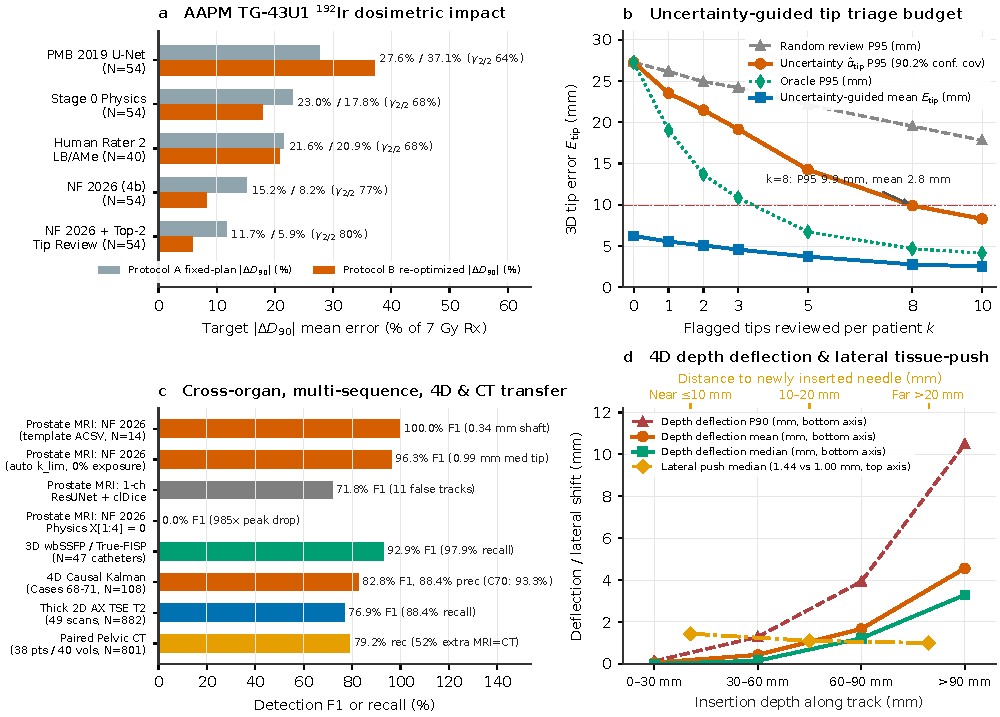
\includegraphics[width=1\linewidth,height=\textheight,keepaspectratio]{../reports/figures/fig8_clinical_translation_and_generalization.pdf}
\caption{\textbf{Clinical translation and cross-domain generalization.}
\textbf{(a) AAPM TG-43U1 \(^{192}\text{Ir}\) dosimetric accuracy} across
54 patients under Protocol A (fixed reference dwell plan transferred to
predicted catheters, grey bars) and Protocol B (dwell times re-optimized
on predicted catheters and delivered to the true anatomy, vermilion bars
with white circles marking the median), alongside 3D
\(\gamma(2\%/2\text{ mm})\) pass rates (\texttt{*} = simulated 2-tip
oracle). \textbf{(b) Simulated clinician tip-review curve:}
95th-percentile and mean 3D tip error as a physicist reviews the top
\(k \in \{0, \dots, 10\}\) tips per patient ranked by predicted
uncertainty \(\hat{\sigma}_{\text{tip}}\) (1-click tip relocation
oracle, vs.~random order and largest-error oracle). \textbf{(c)
Zero-shot generalization} to 3T prostate brachytherapy MRI
(\texttt{Case\ 100}), 3D wbSSFP, thick-slice 2D AX TSE T2, post-contrast
3D T1 VIBE (showing the polarity-shift failure boundary where Stage 0
alone reaches 61.5\% F1 vs.~56.1\% for the T2W-trained full pipeline),
4D intra-procedural causal Kalman tracking (\texttt{Cases\ 68–71}), and
38 paired Pelvic CT cases (40 CT volumes). \textbf{(d) In-vivo 4D
depth-dependent needle bending} across 23 serial scans
(\texttt{Cases\ 68–71}), showing non-linear lateral shaft deflection
versus insertion depth from the template entry. \textbf{(e) In-vivo 4D
lateral ``tissue push'' displacement} of already-implanted catheters as
a function of distance to a newly inserted needle
(\(p = 9.97 \times 10^{-4}\)).}\label{fig:clinical_gen}
\end{figure}

Finally, we asked four practical questions that determine whether an
algorithm is genuinely useful in clinical radiation oncology (summarized
in Table \ref{tbl:clinical_summary} and Figure \ref{fig:clinical_gen},
with complete protocol and sequence breakdowns in Appendix D, Tables
\ref{tbl:dosimetry_generalization} and \ref{tbl:app_generalization}):

\subsubsection{\texorpdfstring{Does geometric accuracy translate into
accurate radiation dose delivery? (Table \ref{tbl:clinical_summary},
Part A; Appendix D, Table \ref{tbl:dosimetry_generalization}; Figure
\ref{fig:clinical_gen}a)}{Does geometric accuracy translate into accurate radiation dose delivery? (Table , Part A; Appendix D, Table ; Figure a)}}\label{does-geometric-accuracy-translate-into-accurate-radiation-dose-delivery-table-part-a-appendix-d-table-figure-a}

Not all catheter errors matter equally to the radiation dose: a tip
error on a peripheral catheter carrying almost zero dwell time has
little effect, whereas a tip error on a heavily weighted catheter inside
the tumor shifts the target dose substantially. Across our 54 patients,
\textbf{dwell-time-weighted 3D tip error}
(\(E_{\text{tip}}^{\text{dwell-w}}\)---the average 3D tip error across a
patient's catheters weighted by each catheter's share of total radiation
dwell time) correlates more strongly with target dose error
\(|\Delta D_{90}|\) than unweighted tip error does (Spearman
\(\rho = 0.863\) vs.~\(0.786\) across the 54 patients; we did not test
the difference between the two correlations).

NeedleFinder 2026 cuts dwell-weighted tip error nearly in half compared
with PMB 2019 (\(5.72\text{ mm}\) vs.~\(10.51\text{ mm}\) mean;
\(4.66\text{ mm}\) vs.~\(8.36\text{ mm}\) median), and is lower than
Human Team 2's on the 40 dual-traced scans (\(5.18\text{ mm}\)
vs.~\(6.27\text{ mm}\) mean; difference not tested). Consequently:

\begin{itemize}
\tightlist
\item
  Under \textbf{Protocol A (transferring a fixed dwell plan)},
  NeedleFinder 2026 cuts mean target dose error \(|\Delta D_{90}|\) from
  \(27.6\%\) (PMB 2019) to \textbf{15.2\%} (median \textbf{11.5\%},
  \(p = 4.9 \times 10^{-6}\)) and achieves a \textbf{76.6\% global 3D
  \(\gamma(2\%/2\text{ mm})\) pass rate} (\textbf{84.3\%} at
  \(\gamma(3\%/3\text{ mm})\))---and lower error than Human Team 2 on
  the 40 dual-traced scans (\(13.5\%\) vs.~\(21.6\%\)
  \(|\Delta D_{90}|\), uncorrected \(p = 0.028\); \(79.0\%\)
  vs.~\(68.1\%\) \(\gamma_{2\%/2\text{mm}}\), uncorrected \(p = 0.011\);
  suggestive, see Methods).
\item
  Under \textbf{Protocol B (clinical workflow: re-optimizing dwell
  weights on the predicted catheters)}, dwell optimization compensates
  for minor longitudinal shifts, cutting unreviewed target
  \(|\Delta D_{90}|\) to \textbf{8.2\% mean / 4.2\% median}
  (vs.~\(37.1\% / 10.2\%\) for Zaffino \emph{et al.} 2019; on the 40
  dual-traced scans, \(7.0\% / 3.2\%\) for NeedleFinder 2026
  vs.~\(20.9\% / 4.0\%\) for Human Team 2). When a simulated physicist
  corrects just the \textbf{top 2 uncertainty-flagged tips per patient}
  (each moved to its reference depth), target \(|\Delta D_{90}|\) drops
  to \textbf{5.9\% mean / 2.8\% median} (paired Wilcoxon
  \(p = 2.4 \times 10^{-5}\); improved in 37 of 54 patients, worse in 8,
  unchanged in 9), and the global \(\gamma_{2\%/2\text{mm}}\) pass rate
  rises from \(66.0\%\) to \(74.3\%\) (\(p = 9.5 \times 10^{-7}\);
  \(78.2\%\) on the 40 dual-traced scans). Gamma against the reference
  plan is lower under Protocol B than under Protocol A because a
  re-optimized plan is a different dose distribution, not a worse one.
\item
  \textbf{Organ-at-risk proxy doses under Protocol B.} Because the
  re-optimized plan is a different plan, dose to the proxy organ shells
  moves more than the target dose does. Across the 54 patients, the
  unreviewed \(|\Delta D_{2\text{cc}}|\) on the bladder, rectum, and
  sigmoid proxy shells is \(17.5\%\), \(18.3\%\), and \(12.5\%\) median
  (\(24.6\%\), \(26.2\%\), and \(29.5\%\) mean); correcting the two most
  uncertain tips lowers these to \(13.7\%\), \(13.1\%\), and \(10.1\%\)
  median (\(17.8\%\), \(19.4\%\), and \(22.5\%\) mean). These shells sit
  5.5 to 16 mm from the implant, in the steepest part of the
  \(^{192}\text{Ir}\) dose gradient, and are not patient anatomy, so the
  percentages are not clinical \(D_{2\text{cc}}\) values. On the same
  shells and the same 40 dual-traced scans, Human Team 2's traces give
  \(19.9\%\) (bladder) and \(25.2\%\) (rectum) median against
  NeedleFinder 2026's \(14.3\%\) and \(11.4\%\). Under Protocol A (fixed
  plan transferred), the bladder and rectum proxy differences are
  \(3.8\%\) and \(5.4\%\) median (Table \ref{tbl:clinical_summary};
  Appendix D, Table \ref{tbl:dosimetry_generalization}).
\end{itemize}

\subsubsection{\texorpdfstring{Can calibrated uncertainty intervals
guide a 1-minute clinician tip check? (Table \ref{tbl:clinical_summary},
Part B; Appendix D, Table \ref{tbl:dosimetry_generalization}; Figure
\ref{fig:clinical_gen}b)}{Can calibrated uncertainty intervals guide a 1-minute clinician tip check? (Table , Part B; Appendix D, Table ; Figure b)}}\label{can-calibrated-uncertainty-intervals-guide-a-1-minute-clinician-tip-check-table-part-b-appendix-d-table-figure-b}

Because 98.8\% of tip error lies longitudinally along the already-traced
shaft, correcting an uncertain tip in 3D Slicer requires only sliding
the endpoint along the track (a single click, which we assume takes 8
seconds). Our out-of-fold tip uncertainty score
\(\hat{\sigma}_{\text{tip}}\) identifies \(>10\text{ mm}\) tip outliers
with an \textbf{AUROC of 0.805}, and our nested \textbf{split-conformal
3D prediction intervals} achieve close-to-nominal empirical coverage
across all 54 unseen test patients despite within-patient clustering
(\textbf{79.3\%} at 80\% nominal, \textbf{84.4\%} at 85\%,
\textbf{90.2\% coverage at the 90\% nominal level}, and \textbf{95.4\%
at the 95\% level}, with \(31.5\%\text{--}35.1\%\) tighter median error
bars than unscaled intervals; Table \ref{tbl:clinical_summary}, Part B;
Appendix D, Table \ref{tbl:dosimetry_generalization}, Part B2).

In our simulated clinician-in-the-loop workflow where a physicist
inspects the top \(k\) highest-uncertainty tips per patient and clicks
the true distal termination (Table \ref{tbl:clinical_summary}, Part B;
Appendix D, Table \ref{tbl:dosimetry_generalization}, Part B1; Figure
\ref{fig:clinical_gen}b):

\begin{itemize}
\tightlist
\item
  Reviewing \textbf{\(k = 2\) tips per patient} (18 s modeled, including
  2 s to open the review list) lowers mean tip error from
  \(6.23\text{ mm}\) to \textbf{\(5.07\text{ mm}\)} (\(1.95\text{ mm}\)
  median).
\item
  Reviewing \textbf{\(k = 5\) tips per patient} (42 s modeled) cuts
  \(>10\text{ mm}\) tip outliers in half (\(16.7\% \to 8.0\%\)) and
  lowers mean tip error to \textbf{\(3.72\text{ mm}\)}
  (\(1.67\text{ mm}\) median).
\item
  Reviewing \textbf{\(k = 8\) tips per patient} (66 s modeled) brings
  the \textbf{95th-percentile tip error across the entire 972-catheter
  cohort below \(10\text{ mm}\) (\(9.90\text{ mm}\)
  vs.~\(27.27\text{ mm}\) unreviewed)} and reduces mean tip error to
  \textbf{\(2.77\text{ mm}\)} (\(1.51\text{ mm}\) median).
\end{itemize}

\subsubsection{\texorpdfstring{Does the method generalize zero-shot to
other organs and MRI sequences? (Table \ref{tbl:clinical_summary}, Part
D; Appendix D, Table \ref{tbl:app_generalization}; Figure
\ref{fig:clinical_gen}c)}{Does the method generalize zero-shot to other organs and MRI sequences? (Table , Part D; Appendix D, Table ; Figure c)}}\label{does-the-method-generalize-zero-shot-to-other-organs-and-mri-sequences-table-part-d-appendix-d-table-figure-c}

To test whether NeedleFinder 2026 overfits to gynecologic T2W MRI, we
ran the gynecologic-trained models \textbf{zero-shot (with zero
retraining)} across three new settings:

\begin{itemize}
\tightlist
\item
  \textbf{Cross-organ transfer to 3T prostate brachytherapy MRI
  (\texttt{Case\ 100}, 14 plastic needles):} This prostate scan is one
  of the 51 external volumes used, without labels, for Stage 1
  pre-training, so we first evaluate a variant pre-trained without it
  (the zero-exposure row of Table \ref{tbl:clinical_summary}, Part D,
  and Appendix D, Table \ref{tbl:app_generalization}). With automatic
  template cropping, that variant found \textbf{13 of 14 prostate
  catheters with no false alarms (96.3\% F1)}, with
  \textbf{\(0.33\text{ mm}\) median shaft error} and
  \textbf{\(0.99\text{ mm}\) median 3D tip error}; with the clinician's
  manual crop it found all 14. The full pipeline, whose pre-training had
  seen this scan without labels, found all 14 under automatic cropping
  (errors in Appendix D, Table \ref{tbl:app_generalization}).
  \textbf{Why does it transfer on this scan?} When we zeroed out the
  Stage 0 physical symmetry channels (\(X_{1:3}=0\)), prostate detection
  collapsed to \textbf{0\% (0/14)}, whereas the 1-channel
  \texttt{ResUNet\ +\ clDice} baseline hallucinated 11 false vascular
  tracks (\(56.0\%\) precision, \(71.8\%\) F1). Thus, on this single
  scan, the Stage 0 physical symmetry channels carried the transfer from
  gynecologic to prostate anatomy.
\item
  \textbf{Secondary MRI pulse sequences (63 of the 243 secondary scans
  evaluated):} On 3D balanced steady-state free precession
  (\texttt{3D\ wbSSFP\ /\ True-FISP}), where tissue contrast differs
  markedly from TSE T2W, zero-shot NeedleFinder 2026 achieved
  \textbf{97.9\% recall (\(46/47\)), 88.5\% precision, and 92.9\% F1}
  (\(0.72\text{ mm}\) median shaft error, \(3.40\text{ mm}\) median tip
  error vs.~\(10.62\text{ mm}\) for PMB 2019). On 49 thick-slice 2D
  axial T2W scans (\(\Delta z = 2.4\text{--}6.0\text{ mm}\)),
  Z-upsampling to \(1.6\text{ mm}\) recovered \textbf{88.4\%
  (\(780/882\)) of physically visible catheters} (\(76.9\%\) F1
  vs.~\(57.6\%\) for clDice). On the third secondary sequence we
  evaluated, 12 post-contrast axial T1 VIBE scans from 2 patients (217
  catheters), zero-shot F1 fell to \(56.1\%\) (\(58.5\%\) recall,
  \(53.8\%\) precision, \(8.08\text{ mm}\) median tip error), below
  Stage 0 alone (\(61.5\%\)) and the 2019 U-Net + DBSCAN
  re-implementation (\(59.4\%\)): post-contrast T1 catheter contrast
  lies outside what the pipeline was trained on.
\item
  \textbf{Zero-shot tracking on post-implant Pelvic CT (40 CT volumes,
  38 paired patients):} Extending Stage 0 to detect both bright metallic
  stylets and dark air lumens in Hounsfield units enabled zero-shot CT
  reconstruction across 801 MRI-paired reference catheters, matching
  \textbf{68.9\% at \(\le 3.5\text{ mm}\) and 79.2\% at
  \(\le 5.0\text{ mm}\)} across non-rigid MRI-to-CT anatomical
  deformation (\(2.01\text{ mm}\) median shaft registration residual).
\end{itemize}

\subsubsection{\texorpdfstring{Can we track needles across serial scans
during insertion and measure tissue biomechanics in 4D? (Table
\ref{tbl:clinical_summary}, Part D; Appendix D, Table
\ref{tbl:app_generalization}; Figure \ref{fig:clinical_gen}c, d,
e)}{Can we track needles across serial scans during insertion and measure tissue biomechanics in 4D? (Table , Part D; Appendix D, Table ; Figure c, d, e)}}\label{can-we-track-needles-across-serial-scans-during-insertion-and-measure-tissue-biomechanics-in-4d-table-part-d-appendix-d-table-figure-c-d-e}

In 4 patients (\texttt{Cases\ 68–71}), 23 sequential T2W scans were
acquired \emph{during} the implant procedure as needles were
progressively inserted (5 to 7 timepoints per patient, \(1.31\text{ s}\)
mean monitoring runtime per scan). Evaluating each patient's 4D series
strictly with the outer-fold model where that patient was held out in
the locked test vault (\texttt{Case\ 068} in Fold 4, \texttt{Case\ 069}
in Fold 0, \texttt{Case\ 070} in Fold 1, \texttt{Case\ 071} in Fold 2),
coupling NeedleFinder 2026 with a \textbf{causal 4D Kalman filter} that
propagates catheter states forward in time boosted \textbf{pooled
precision across the 108 catheters by +12.4 percentage points
(\(76.0\% \to 88.4\%\))}, reduced mean 3D tip error from
\(11.23\text{ to }9.75\text{ mm}\), and improved pooled F1 from
\textbf{81.6\% to 82.8\%}, a difference we did not test given only 4
patients (reaching \textbf{93.3\% F1} on \texttt{Case\ 070}, up from
\(85.7\%\) with independent 3D tracking, while trading single-frame
recall on newly inserted final-frame needles in \texttt{Case\ 071} for
\(100.0\%\) precision).

Tracking \(212\) persisted catheter transitions across these sequential
insertions, measured on the automatically tracked catheters rather than
on expert traces, also suggested two biomechanical patterns in vivo
(Figure \ref{fig:clinical_gen}d, e):

\begin{itemize}
\tightlist
\item
  \textbf{Inter-catheter ``tissue push'':} Inserting a new needle
  appears to push surrounding soft tissue aside. Already-implanted
  catheters located within \(\le 10\text{ mm}\) of a newly inserted
  needle shifted sideways by a \textbf{median of \(1.44\text{ mm}\)}
  (mean \(1.61\text{ mm}\), 90th percentile \(2.81\text{ mm}\)),
  compared with \textbf{\(1.10\text{ mm}\)} at
  \(10\text{--}20\text{ mm}\) distance and \textbf{\(1.00\text{ mm}\)}
  beyond \(20\text{ mm}\) (Mann--Whitney test of catheters within
  \(12\text{ mm}\) versus beyond \(12\text{ mm}\),
  \(p = 9.97 \times 10^{-4}\); the 212 transitions come from 4 patients
  and are treated as independent, so this \(p\)-value is optimistic).
\item
  \textbf{Depth-dependent needle bending:} Deviation of a catheter from
  its initial entry angle grows non-linearly with insertion depth,
  rising from below measurement resolution at \(0\text{--}30\text{ mm}\)
  depth and \(0.15\text{ mm}\) at \(30\text{--}60\text{ mm}\) to
  \textbf{\(1.22\text{ mm}\) at \(60\text{--}90\text{ mm}\)} and
  \textbf{\(3.29\text{ mm}\) median (\(4.56\text{ mm}\) mean,
  \(10.49\text{ mm}\) P90) beyond \(90\text{ mm}\) depth} (Spearman
  \(\rho = +0.555\) across depth samples pooled from 4 patients, nominal
  \(p = 5.6 \times 10^{-9}\))---one reason to expect linear
  extrapolation of the entry angle to be unreliable on deep pelvic
  implants.
\end{itemize}

\FloatBarrier

\section{Discussion}\label{discussion}

\subsection{Why Combining Physics, Peak Regression, and Graph Reasoning
Works}\label{why-combining-physics-peak-regression-and-graph-reasoning-works}

Appendix C (Table \ref{tbl:literature}) places NeedleFinder 2026 in the
context of published catheter digitization methods across CT,
ultrasound, and MRI. On CT and ultrasound, metallic stylets, air lumens,
or specular reflections create strong contrast against soft tissue,
allowing voxel segmentation networks to reach
\(0.1\text{ to }0.7\text{ mm}\) shaft errors (Andersén \emph{et al.},
2020; Zhang \emph{et al.}, 2020d; Weishaupt \emph{et al.}, 2022; Quetin
\emph{et al.}, 2025; Xiao \emph{et al.}, 2026a). On clinical T2W MRI
without exogenous contrast markers, a plastic catheter is a 2 mm dark
proton-density and susceptibility void imaged across 1.2 to 6.0 mm
slices. Prior MRI studies reported \(0.74\text{ to }0.97\text{ mm}\)
shaft errors on gynecologic implants using positive-contrast markers or
CT-assisted ground truth (Shaaer \emph{et al.}, 2022; Kim \emph{et al.},
2026) and \(0.75\text{ to }0.93\text{ mm}\) on prostate implants (Dai
\emph{et al.}, 2020; Kostoulas \emph{et al.}, 2025). NeedleFinder 2026
reaches a median shaft error below half a millimeter directly on
standard T2W MRI on the 972 matched catheters of a 1,063-catheter cohort
(Table \ref{tbl:main}), although these are different cohorts and
reference standards, so the comparison is indicative only.

Our controlled ablations and peer-reviewed baseline reproductions
explain why neither voxel segmentation (Zaffino \emph{et al.}, 2019;
Isensee \emph{et al.}, 2021; Shit \emph{et al.}, 2021), nor 1-channel
MRI post-processing (Dai \emph{et al.}, 2020; Aleong \emph{et al.},
2024; Kostoulas \emph{et al.}, 2025; Kim \emph{et al.}, 2026), nor
mask-based tracking (Xiao \emph{et al.}, 2026a) suffices on its own on
T2W MRI, and why each part of our three-stage design is needed:

\begin{enumerate}
\def\labelenumi{\arabic{enumi}.}
\tightlist
\item
  \textbf{Local physical symmetry before deep learning:} Stage 0
  suppresses one-sided anatomical borders analytically and provides a
  representation that, on one prostate implant scan and 48 needle-free
  scans, let a gynecologic network transfer zero-shot without
  hallucinating blood vessels.
\item
  \textbf{Centerline peaks and hard-negative pre-training instead of
  binary masks:} By pre-training Stage 1 on 51 external pelvic MRI scans
  where real blood vessels and fascia are penalized as hard negatives
  alongside synthetic catheter voids, and by predicting sharp sub-pixel
  Gaussian peaks (\(P_{\text{peak}}\)) supervised by two expert teams,
  touching catheters stay separate instead of merging into a single
  blob.
\item
  \textbf{Graph message passing, fragment stitching, and bundle-level
  context:} Rather than trusting local voxel connectivity, Stage 2A
  enforces smooth triplet collinearity and stitches fragments across
  1-to-3-slice signal dropouts, while the Stage 2B graph transformer
  judges every candidate trajectory against the geometry of the entire
  15-to-30-catheter bundle.
\item
  \textbf{Dedicated 1D axial tip profiling and literature fusion:}
  Because 98.8\% of tip error is longitudinal along the shaft, sampling
  a fine \(0.5\text{ mm}\) multi-channel profile along the cranial
  trajectory tangent allows a 1D ResNet + self-attention localizer to
  pinpoint where the catheter void terminates and to quantify its own
  uncertainty---while incorporating sub-voxel inverse-variance-weighted
  polynomial fitting (Aleong \emph{et al.}, 2024; Kim \emph{et al.},
  2026), directional axial TV continuity (Dai \emph{et al.}, 2020), and
  iterative multi-segment gap-bridging (Kostoulas \emph{et al.}, 2025)
  refines shaft and tip accuracy and suppresses residual split fragments
  (\texttt{4d}, \textbf{89.4\% F1}).
\end{enumerate}

\subsection{How NeedleFinder 2026 Changes the Clinical Workflow in 3D
Slicer}\label{how-needlefinder-2026-changes-the-clinical-workflow-in-3d-slicer}

Packaged as a one-click module in \textbf{3D Slicer} (Fedorov \emph{et
al.}, 2012), NeedleFinder 2026 runs in a few seconds on a 24-core
workstation CPU or a GPU when its production Rust and ONNX Runtime code
path is run headless, outside the Slicer interface (Figure
\ref{fig:spec_runtime}c). Instead of spending 45 to 50 minutes manually
clicking 15 to 30 catheters slice by slice while the patient waits with
the implant in place, the medical physicist follows a structured
verification workflow that we have modeled, not timed, at about half a
minute for the two-tip check:

\begin{enumerate}
\def\labelenumi{\arabic{enumi}.}
\tightlist
\item
  \textbf{Click \emph{Detect Needles} (4 seconds for the production code
  path run headless; interface overhead not yet timed):} The software
  crops the template plane automatically and reconstructs the 3D
  catheter bundle. Because our non-inferiority analysis shows that the
  reconstructed shafts (Table \ref{tbl:interobserver}) are statistically
  non-inferior to human inter-observer agreement with Team 1 as
  reference, this modeled workflow assumes no manual shaft editing; we
  did not measure how often shafts are edited.
\item
  \textbf{Check the few tips with the widest uncertainty bars (18 to 66
  seconds simulated):} The module is designed to list the catheter tips
  with the widest split-conformal uncertainty intervals
  (\(\hat{\sigma}_{\text{tip}}\)) first. Because the shaft is already
  traced, correcting a flagged tip means sliding its endpoint along the
  track, which we model at 8 seconds per tip. Correcting only the two
  most uncertain tips per patient (18 seconds) is the configuration we
  carried through the TG-43U1 dose simulation: it lowers median target
  dose error \(|\Delta D_{90}|\) from 4.2\% to \textbf{2.8\%} (mean from
  8.2\% to 5.9\%). Extending the check to the eight most uncertain tips
  (66 seconds) was evaluated on tip geometry only; it brings the
  95th-percentile tip error below \(10\text{ mm}\) (\(9.90\text{ mm}\),
  mean \(2.77\text{ mm}\)). In the dose simulation the flagged tip is
  placed exactly at its reference depth; in the tip-geometry curve a
  residual of up to \(0.85\text{ mm}\) along the shaft is retained.
  Either way the simulated physicist never errs, so these numbers are
  upper bounds on the benefit of review.
\item
  \textbf{Reconcile the catheter count (assumed 5 seconds):} The
  clinician knows how many needles went through the template
  (\(N_{\text{implant}}\)). If the software reports more, the physicist
  deletes the extra tracks (2.7 unmatched predictions per patient at the
  default threshold, of which 1.2 are genuine false alarms on vessels or
  fascia); we did not simulate this deletion, and the Protocol B dose
  simulation loads every predicted track, so its unreviewed numbers
  include these tracks. If the software reports fewer, one click near
  the missing catheter promotes the highest-scoring candidate track that
  Stage 2B had rejected there, rather than tracing from scratch. Only
  misses that still exist in the Stage 2A candidate pool can be
  recovered this way, so in simulation \(0.65\) such promotions per
  patient raise 1-to-1 recall from 91.4\% to \textbf{93.0\%} (\(94.2\%\)
  closest-match recall) at the cost of 18 additional false tracks
  (precision \(86.9\% \to 85.8\%\)). Moreover, during progressive needle
  insertion in intraoperative MRI suites, the \(1.31\text{ s}\) causal
  4D Kalman mode could in principle alert the implanting physician after
  each interim scan if a newly inserted needle pushes a neighboring
  catheter out of position or deflects toward an organ at risk; we
  evaluated it only retrospectively on 23 scans from 4 patients.
\end{enumerate}

\subsection{Limitations and Future
Directions}\label{limitations-and-future-directions}

Four limitations of the present study point directly to future work:

\begin{enumerate}
\def\labelenumi{\arabic{enumi}.}
\tightlist
\item
  \textbf{Longitudinal tip ambiguity on thick slices.} While our 1D
  axial tip localizer cuts mean tip error to \(6.23\text{ mm}\) and
  median tip error to \(2.26\text{--}2.27\text{ mm}\)
  (\(58.7\%\text{--}59.0\%\) within \(\le 3.0\text{ mm}\)), \(16.7\%\)
  of unreviewed catheters still have a longitudinal tip error exceeding
  \(10\text{ mm}\) when a catheter passes through a multi-slice signal
  dropout or terminates directly beneath dark bowel gas on 3 to 6 mm
  thick slices. Although simulated uncertainty-guided review of 5 to 8
  tips contains this tail in our oracle model, combining T2W planning
  scans with thin-slice isotropic 3D sequences (\(\le 1\text{ mm}\)) or
  zero-echo-time sequences (Kaza \emph{et al.}, 2022; Lee \emph{et al.},
  2023) is the natural path to reducing unreviewed tip outliers further.
\item
  \textbf{Single-institution clinical implant cohort.} While we tested
  zero-shot transfer on 48 external public prostate scans, one 3T
  prostate brachytherapy MRI, three other MRI pulse sequences, 4D
  insertion series, and paired CT scans, all implanted brachytherapy
  patients were treated at Brigham and Women's Hospital. Prospective
  multi-center validation across 1.5T, 3T, and emerging low-field MRI
  systems (Major \emph{et al.}, 2026) from multiple scanner vendors is
  the essential next step.
\item
  \textbf{Standardized TG-43U1 anatomical envelopes and simulated review
  timings.} Because clinical DICOM RTSTRUCT and RTPLAN files were not
  archived across the historical 54-patient repository, our TG-43U1
  dosimetric study used standardized target and organ-at-risk envelopes
  derived from the active implant geometry; the organ-at-risk shells lie
  in the steepest part of the dose gradient, which is why their proxy
  \(D_{2\text{cc}}\) differences are several times larger than the
  target \(D_{90}\) differences and must not be read as clinical organ
  doses. Our clinician tip-review curves used a quantitative 1-click
  oracle rather than prospective stopwatch trials in the operating room.
\item
  \textbf{Role of synthetic bundle pre-training
  (\texttt{SynthBrachy3T}).} Once Stage 1 is pre-trained on 51 external
  pelvic MRI scans and paired with collinear fragment stitching and the
  1D tip localizer, \texttt{SynthBrachy3T} provides its largest
  detection boost when clinical bundle labels are scarce
  (\(k = 0\text{ to }5\) patients, lifting zero-shot long-shaft
  \(F1_{\text{adj}}\) by \(+6.3\) points to \(83.4\%\)), while offering
  a smaller refinement at the full 43-patient training budget (\(+0.4\)
  F1 points, while reducing dwell-weighted tip error from
  \(6.65\text{ to }5.72\text{ mm}\) and counterfactual
  \(|\Delta D_{90}|\) from \(12.8\%\text{ to }8.2\%\)).
\end{enumerate}

\FloatBarrier

\section{Conclusion}\label{conclusion}

NeedleFinder 2026 reconstructs interstitial brachytherapy catheters
directly on clinical 3T T2-weighted MRI. It combines an analytical
dark-core symmetry filter (Stage 0), a 3D U-Net pre-trained on
needle-free pelvic scans and fine-tuned on two expert teams' traces
(Stage 1), and graph tracking with bundle-level scoring and a 1D axial
tip localizer (Stage 2). Under strictly nested cross-validation on 54
patients and 1,063 catheters, it finds about nine catheters in ten with
a median shaft error below half a millimeter and a median tip error of
about 2 mm, in a few seconds on a workstation CPU (Table \ref{tbl:main};
Figure \ref{fig:spec_runtime}), and it outperforms our
re-implementations of five peer-reviewed methods and one tracking
preprint on the same splits. On 40 doubly traced scans its disagreement
with one expert team is no larger than the disagreement between the two
teams, and paired post-implant CT confirms that half of its apparent
false alarms are real catheters (Table \ref{tbl:interobserver}). Its
calibrated tip uncertainty supports a brief simulated check in 3D
Slicer: moving the two most uncertain tips per patient to their
reference depth, modeled at 18 seconds, lowers simulated target dose
error from 4.2\% to 2.8\% median (Table \ref{tbl:clinical_summary};
Appendix D, Table \ref{tbl:dosimetry_generalization}). Without
retraining, the pipeline also runs on one prostate implant, two other
T2-type MRI sequences, serial intra-procedural scans and, with lower
recall, post-contrast T1 MRI and pelvic CT.

\FloatBarrier

\section*{Data Availability}\label{data-availability}
\addcontentsline{toc}{section}{Data Availability}

The 54 clinical MRI scans and their expert annotations were acquired at
Brigham and Women's Hospital under Institutional Review Board approval
and contain protected health information; they cannot be shared
publicly. De-identified trajectory annotations and per-patient
evaluation results may be made available by the corresponding author
upon reasonable request, subject to institutional ethics approval. The
48 needle-free pelvic MRI scans are publicly available from the Medical
Segmentation Decathlon (\texttt{Task05\_Prostate},
http://medicaldecathlon.com (Antonelli \emph{et al.}, 2022)). The
\texttt{SynthBrachy3T} synthetic bundle generator is released with our
open-source repository.

\section*{Code Availability}\label{code-availability}
\addcontentsline{toc}{section}{Code Availability}

The 3D Slicer extension, the native Rust Stage 0 kernel
(\texttt{needlefinder\_rust}), and the exported ONNX models
(\texttt{NeedleUNet3D}, \texttt{NeedleSliceMPNN},
\texttt{TipAwareBundleGraphTransformer}, and
\texttt{Dedicated1DTipLocalizer}) are available at
https://github.com/needlefinder/NeedleFinder under an open-source
license. All scripts for reference-free preprocessing
(\texttt{prepare\_clean\_dataset.py}), self-supervised pre-training
(\texttt{pretrain\_ssl\_unet3d.py}), strictly nested \(5 \times 5\)
training and evaluation (\texttt{train\_nested\_stage1.py},
\texttt{run\_stage2\_and\_tip\_clean.py},
\texttt{export\_clean\_unified\_and\_table3.py}), peer-reviewed baseline
reproduction and literature fusion
(\texttt{run\_part1\_peer\_baselines\_and\_unc\_maps.py},
\texttt{run\_part2\_literature\_fusion\_inside\_needlefinder.py}),
specificity benchmarking
(\texttt{benchmark\_public\_pelvic\_mri\_clean.py}), runtime profiling
(\texttt{benchmark\_54cases\_timing\_clean.py}), calibration and failure
auditing (\texttt{calibration\_and\_failure\_clean.py}), and clinical
translation Experiments 1--4 (\texttt{run\_exp1\_tg43\_dosimetry.py}
through \texttt{run\_exp4\_4d\_insertion\_and\_ct.py}) are archived in
the \texttt{benchmarks\_clean/} directory of the repository.

\section*{Ethics Statement}\label{ethics-statement}
\addcontentsline{toc}{section}{Ethics Statement}

This retrospective study analyzed imaging data acquired during routine
clinical care under a protocol approved by the Institutional Review
Board of Brigham and Women's Hospital / Mass General Brigham.

\section*{Funding}\label{funding}
\addcontentsline{toc}{section}{Funding}

{[}Funding sources and grant numbers to be inserted.{]}

\section*{Acknowledgments}\label{acknowledgments}
\addcontentsline{toc}{section}{Acknowledgments}

The authors thank the clinical physics, radiation oncology, and
radiology staff of the AMIGO suite at Brigham and Women's Hospital for
their support in data acquisition and clinical annotation.

\section*{Author Contributions}\label{author-contributions}
\addcontentsline{toc}{section}{Author Contributions}

{[}To be completed following the CRediT taxonomy.{]}

\section*{Conflicts of Interest}\label{conflicts-of-interest}
\addcontentsline{toc}{section}{Conflicts of Interest}

The authors declare no conflicts of interest.

\section*{Declaration of Generative AI and AI-Assisted
Technologies}\label{declaration-of-generative-ai-and-ai-assisted-technologies}
\addcontentsline{toc}{section}{Declaration of Generative AI and
AI-Assisted Technologies}

During the preparation of this work the authors used large language
models (Anthropic Claude, OpenAI ChatGPT and Codex, and Google Gemini)
for four tasks: verifying bibliographic details and reported figures of
cited literature against the original publications; organizing and
restructuring the manuscript; editing language for clarity and
readability; and adversarially reviewing draft sections, tables, and
evaluation scripts for errors, inconsistencies, and unsupported claims.
These tools did not design the method, acquire or annotate the data, run
the experiments, or generate any result reported here. After using these
tools, the authors reviewed and edited every sentence, re-derived every
number from the archived benchmark outputs, and take full responsibility
for the content of the publication. No AI tool is listed as an author,
in accordance with Elsevier, IOP Publishing, and ICMJE authorship
policies.

\section*{References}\label{references}
\addcontentsline{toc}{section}{References}

\phantomsection\label{refs}
\begin{CSLReferences}{1}{1}
\bibitem[\citeproctext]{ref-aleong2024}
Aleong, A.M., Berlin, A., Borg, J., Helou, J., Beiki-Ardakani, A., Rink,
A., Raman, S., Chung, P., and Weersink, R.A. 2024. Rapid multi-catheter
segmentation for magnetic resonance image-guided catheter-based
interventions. \emph{Medical Physics}, \textbf{51}, 5361--73.
\url{https://doi.org/10.1002/mp.17117}.

\bibitem[\citeproctext]{ref-andersen2020}
Andersén, C., Rydén, T., Thunberg, P., and Lagerlöf, J.H. 2020. Deep
learning-based digitization of prostate brachytherapy needles in
ultrasound images. \emph{Medical Physics}, \textbf{47}, 6414--20.
\url{https://doi.org/10.1002/mp.14508}.

\bibitem[\citeproctext]{ref-androulakis2025}
Androulakis, I., Godart, J., Luthart, L., MEMC, C., Westerveld, H.,
Nout, R.A., Hoogeman, M., and Kolkman-Deurloo, I.K. 2025. Reconstruction
errors in clinical intraoperative TRUS-based prostate HDR-BT detected
using electromagnetic tracking. \emph{Brachytherapy}, \textbf{24},
177--85. \url{https://doi.org/10.1016/j.brachy.2024.11.004}.

\bibitem[\citeproctext]{ref-antonelli2022}
Antonelli, M., Reinke, A., Bakas, S., Farahani, K., Kopp-Schneider, A.,
Landman, B.A., Litjens, G., Menze, B., Ronneberger, O., Summers, R.M.,
et al. 2022. The medical segmentation decathlon. \emph{Nature
Communications}, \textbf{13}, 4128.
\url{https://doi.org/10.1038/s41467-022-30695-9}.

\bibitem[\citeproctext]{ref-arapi2023}
Arapi, V., Hardt-Stremayr, A., Weiss, S., and Steinbrener, J. 2023.
Bridging the simulation-to-real gap for {AI}-based needle and target
detection in robot-assisted ultrasound-guided interventions.
\emph{European Radiology Experimental}, \textbf{7}, 30.
\url{https://doi.org/10.1186/s41747-023-00344-x}.

\bibitem[\citeproctext]{ref-dearcos2017}
Arcos, J. de, Schmidt, E.J., Wang, W., Tokuda, J., Vij, K., Seethamraju,
R.T., Damato, A.L., Dumoulin, C.L., Cormack, R.A., and Viswanathan, A.N.
2017. Prospective clinical implementation of a novel magnetic resonance
tracking device for real-time brachytherapy catheter positioning.
\emph{International journal of radiation oncology, biology, physics},
\textbf{99}, 618--26.
\url{https://doi.org/10.1016/j.ijrobp.2017.05.054}.

\bibitem[\citeproctext]{ref-beaulieu2025}
Beaulieu, L., Bert, C., Borot de Battisti, M., Cormack, R.A., Cunha,
J.A.M., Damato, A.L., Deufel, C.L., Hautvast, G.L.T.F., Hsu, I.-C.,
Kolkman-Deurloo, I.-K., Moerland, M.A., Niatsetski, Y., Weersink, R.A.,
and Tanderup, K. 2025. {AAPM} task group 317 report: A joint {AAPM} and
{ESTRO} report on brachytherapy catheter, needle, and applicator
tracking technology. \emph{Medical Physics}, \textbf{52}, e70037.
\url{https://doi.org/10.1002/mp.70037}.

\bibitem[\citeproctext]{ref-benhaim2022}
Ben-Haim, T., and Riklin Raviv, T. 2022. Graph neural network for cell
tracking in microscopy videos. \emph{Computer vision -- ECCV 2022},
Lecture notes in computer science, vol 13681, (Springer), pp 610--26.
\url{https://doi.org/10.1007/978-3-031-19803-8_36}.

\bibitem[\citeproctext]{ref-braso2020}
Brasó, G., and Leal-Taixé, L. 2020. Learning a neural solver for
multiple object tracking. \emph{Proceedings of the IEEE/CVF conference
on computer vision and pattern recognition (CVPR)}, pp 6246--56.
\url{https://doi.org/10.1109/CVPR42600.2020.00628}.

\bibitem[\citeproctext]{ref-kirisits2014}
C, K., MJ, R., D, B., F, B., M, D.B., Laarse R, van der, Y, N., P, P.,
TP, H., J, P.-C., K, T., JL, V., and FA, S. 2014. Review of clinical
brachytherapy uncertainties: Analysis guidelines of GEC-ESTRO and the
AAPM. \emph{Radiotherapy and oncology : journal of the European Society
for Therapeutic Radiology and Oncology}, \textbf{110}, 199--212.
\url{https://doi.org/10.1016/j.radonc.2013.11.002}.

\bibitem[\citeproctext]{ref-cantin2024}
Cantin, A., Lavallée, M.-C., Poulin, E., Hautvast, G., Foster, W., and
Beaulieu, L. 2024. Proof-of-concept of real-time electromagnetic
guidance for gynecologic interstitial catheters in high dose rate
brachytherapy. \emph{Physics and Imaging in Radiation Oncology},
\textbf{32}, 100661. \url{https://doi.org/10.1016/j.phro.2024.100661}.

\bibitem[\citeproctext]{ref-chen2014}
Chen, X., and Egger, J. 2014. Development of an open source software
module for enhanced visualization during MR-guided interstitial
gynecologic brachytherapy. \emph{SpringerPlus}, \textbf{3}, 167.
\url{https://doi.org/10.1186/2193-1801-3-167}.

\bibitem[\citeproctext]{ref-chino2025}
Chino, J., Erickson, B., Gaffney, D., Hsu, I.-C., Kamrava, M., Kim, Y.,
Niedermayr, T.R., Roumeliotis, M., Rownd, J., Todor, D., Viswanathan,
A., and Kidd, E.A. 2025. The {American Brachytherapy Society} ({ABS})
consensus guidance for hybrid intracavitary interstitial brachytherapy
for locally advanced cervical cancer. \emph{Brachytherapy}, \textbf{24},
463--78. \url{https://doi.org/10.1016/j.brachy.2025.05.001}.

\bibitem[\citeproctext]{ref-dai2020}
Dai, X., Lei, Y., Zhang, Y., Qiu, R.L.J., Wang, T., Dresser, S.A.,
Curran, W.J., Patel, P., Liu, T., and Yang, X. 2020. Automatic
multi-catheter detection using deeply supervised convolutional neural
network in {MRI}-guided high-dose-rate prostate brachytherapy.
\emph{Medical Physics}, \textbf{47}, 4115--24.
\url{https://doi.org/10.1002/mp.14307}.

\bibitem[\citeproctext]{ref-deufel2024}
Deufel, C.L., Brost, E.E., Dupere, J.M., Petersen, I.A., Haddock, M.G.,
and Garda, A.E. 2024. {EMVision}: An electromagnetic tracking guidance
system for accurate placement of interstitial brachytherapy applicators.
\emph{Brachytherapy}, \textbf{23}, 676--86.
\url{https://doi.org/10.1016/j.brachy.2024.06.006}.

\bibitem[\citeproctext]{ref-deufel2020}
Deufel, C.L., Tian, S., Yan, B.B., Vaishnav, B.D., Haddock, M.G., and
Petersen, I.A. 2020. Automated applicator digitization for
high-dose-rate cervix brachytherapy using image thresholding and
density-based clustering. \emph{Brachytherapy}, \textbf{19}, 111--8.
\url{https://doi.org/10.1016/j.brachy.2019.09.002}.

\bibitem[\citeproctext]{ref-dise2015}
Dise, J., Liang, X., Scheuermann, J., Anamalayil, S., Mesina, C., Lin,
L.L., and Teo, B.K. 2015. Development and evaluation of an automatic
interstitial catheter digitization tool for adaptive high-dose-rate
brachytherapy. \emph{Brachytherapy}, \textbf{14}, 619--25.
\url{https://doi.org/10.1016/j.brachy.2015.05.004}.

\bibitem[\citeproctext]{ref-durrbeck2022}
Dürrbeck, C., Sauer, B.C., Lotter, M., Kreppner, S., Strnad, V.,
Fietkau, R., and Bert, C. 2022. Automating implant reconstruction in
interstitial brachytherapy of the breast: A hybrid approach combining
electromagnetic tracking and image segmentation. \emph{Radiotherapy and
Oncology}, \textbf{176}, 172--8.
\url{https://doi.org/10.1016/j.radonc.2022.09.019}.

\bibitem[\citeproctext]{ref-fedorov2012}
Fedorov, A., Beichel, R., Kalpathy-Cramer, J., Finet, J., Fillion-Robin,
J.-C., Pujol, S., Bauer, C., Jennings, D., Fennessy, F., Sonka, M., et
al. 2012. {3D Slicer} as an image computing platform for the
quantitative imaging network. \emph{Magnetic Resonance Imaging},
\textbf{30}, 1323--41. \url{https://doi.org/10.1016/j.mri.2012.05.001}.

\bibitem[\citeproctext]{ref-goulet2025}
Goulet, M., Duguay-Drouin, P., Mascolo-Fortin, J., Mégrourèche, J.,
Octave, N., and Tsui, J.M.G. 2025. Clinical application of deep
learning-assisted needles reconstruction in prostate ultrasound
brachytherapy. \emph{International Journal of Radiation Oncology,
Biology, Physics}, \textbf{122}, 199--207.
\url{https://doi.org/10.1016/j.ijrobp.2024.12.026}.

\bibitem[\citeproctext]{ref-hellebust2010}
Hellebust, T.P., Kirisits, C., Berger, D., Pérez-Calatayud, J., De
Brabandere, M., De Leeuw, A., Dumas, I., Hudej, R., Lowe, G., Wills, R.,
and Tanderup, K. 2010. Recommendations from gynaecological ({GYN})
{GEC-ESTRO} working group: Considerations and pitfalls in commissioning
and applicator reconstruction in {3D} image-based treatment planning of
cervix cancer brachytherapy. \emph{Radiotherapy and Oncology},
\textbf{96}, 153--60.
\url{https://doi.org/10.1016/j.radonc.2010.06.004}.

\bibitem[\citeproctext]{ref-hrinivich2019}
Hrinivich, W.T., Morcos, M., Viswanathan, A., and Lee, J. 2019.
Automatic tandem and ring reconstruction using {MRI} for cervical cancer
brachytherapy. \emph{Medical Physics}, \textbf{46}, 4324--32.
\url{https://doi.org/10.1002/mp.13730}.

\bibitem[\citeproctext]{ref-hu2021}
Hu, H., Yang, Q., Li, J., Wang, P., Tang, B., Wang, X., and Lang, J.
2021. Deep learning applications in automatic segmentation and
reconstruction in {CT}-based cervix brachytherapy. \emph{Journal of
Contemporary Brachytherapy}, \textbf{13}, 325--30.
\url{https://doi.org/10.5114/jcb.2021.106118}.

\bibitem[\citeproctext]{ref-hu2019}
Hu, X., Li, F., Samaras, D., and Chen, C. 2019. Topology-preserving deep
image segmentation. \emph{Advances in neural information processing
systems 32 (NeurIPS 2019)}, vol 32. URL:
\url{https://papers.nips.cc/paper/8803-topology-preserving-deep-image-segmentation}.

\bibitem[\citeproctext]{ref-isensee2021}
Isensee, F., Jaeger, P.F., Kohl, S.A.A., Petersen, J., and Maier-Hein,
K.H. 2021. {nnU-Net}: A self-configuring method for deep learning-based
biomedical image segmentation. \emph{Nature Methods}, \textbf{18},
203--11. \url{https://doi.org/10.1038/s41592-020-01008-z}.

\bibitem[\citeproctext]{ref-richart2015}
J, R., A, O., S, R., AI, N., M, D., M, S., J, V., F, B., and J, P.-C.
2015. A practical MRI-based reconstruction method for a new endocavitary
and interstitial gynaecological template. \emph{Journal of contemporary
brachytherapy}, \textbf{7}, 407--14.
\url{https://doi.org/10.5114/jcb.2015.55340}.

\bibitem[\citeproctext]{ref-jacobsen2022}
Jacobsen, M.C., Beriwal, S., Dyer, B.A., Klopp, A.H., Lee, S.I.,
McGinnis, G.J., Robbins, J.B., Rauch, G.M., Sadowski, E.A., Simiele,
S.J., Stafford, R.J., Taunk, N.K., Yashar, C.M., and Venkatesan, A.M.
2022. Contemporary image-guided cervical cancer brachytherapy: Consensus
imaging recommendations from the society of abdominal radiology and the
american brachytherapy society. \emph{Brachytherapy}, \textbf{21},
369--88. \url{https://doi.org/10.1016/j.brachy.2022.04.005}.

\bibitem[\citeproctext]{ref-dimopoulos2012}
JC, D., P, P., K, T., P, P., D, B., C, K., EM, P., Limbergen E, van, C,
H.-M., and R, P. 2012. Recommendations from gynaecological (GYN)
GEC-ESTRO working group (IV): Basic principles and parameters for MR
imaging within the frame of image based adaptive cervix cancer
brachytherapy. \emph{Radiotherapy and oncology : journal of the European
Society for Therapeutic Radiology and Oncology}, \textbf{103}, 113--22.
\url{https://doi.org/10.1016/j.radonc.2011.12.024}.

\bibitem[\citeproctext]{ref-jung2019b}
Jung, H., Gonzalez, Y., Shen, C., Klages, P., Albuquerque, K., and Jia,
X. 2019a. Deep-learning-assisted automatic digitization of applicators
in 3D CT image-based high-dose-rate brachytherapy of gynecological
cancer. \emph{Brachytherapy}, \textbf{18}, 841--51.
\url{https://doi.org/10.1016/j.brachy.2019.06.003}.

\bibitem[\citeproctext]{ref-jung2019}
Jung, H., Shen, C., Gonzalez, Y., Albuquerque, K., and Jia, X. 2019b.
Deep-learning assisted automatic digitization of interstitial needles in
{3D} {CT} image based high dose-rate brachytherapy of gynecological
cancer. \emph{Physics in Medicine \& Biology}, \textbf{64}, 215003.
\url{https://doi.org/10.1088/1361-6560/ab3fcb}.

\bibitem[\citeproctext]{ref-kallis2019}
Kallis, K., Kaltsas, T., Kreppner, S., Lotter, M., Strnad, V., Fietkau,
R., and Bert, C. 2019. Impact of inter- and intra-observer variabilities
of catheter reconstruction on multi-catheter interstitial brachytherapy
of breast cancer patients. \emph{Radiotherapy and Oncology},
\textbf{135}, 25--32.
\url{https://doi.org/10.1016/j.radonc.2019.02.017}.

\bibitem[\citeproctext]{ref-kapur2012}
Kapur, T., Egger, J., Damato, A., Schmidt, E.J., and Viswanathan, A.N.
2012. 3-t MR-guided brachytherapy for gynecologic malignancies.
\emph{Magnetic resonance imaging}, \textbf{30}, 1279--90.
\url{https://doi.org/10.1016/j.mri.2012.06.003}.

\bibitem[\citeproctext]{ref-karius2024}
Karius, A., Kreppner, S., Strnad, V., Schweizer, C., Lotter, M.,
Fietkau, R., and Bert, C. 2024. Inter-observer effects in needle
reconstruction for temporary prostate brachytherapy: Dosimetric
implications and adaptive {CBCT-TRUS} registration solutions.
\emph{Brachytherapy}, \textbf{23}, 421--32.
\url{https://doi.org/10.1016/j.brachy.2024.05.002}.

\bibitem[\citeproctext]{ref-kaza2022}
Kaza, E., Lee, C.Y., King, M.T., Dyer, M.A., Cormack, R.A., and
Buzurovic, I. 2022. First pointwise encoding time reduction with radial
acquisition (PETRA) implementation for catheter detection in
interstitial high-dose-rate (HDR) brachytherapy. \emph{Brachytherapy},
\textbf{21}, 501--10.
\url{https://doi.org/10.1016/j.brachy.2022.01.003}.

\bibitem[\citeproctext]{ref-kim2026}
Kim, G., Antaki, M., Schmidt, E.J., Roumeliotis, M., Viswanathan, A.N.,
and Lee, J. 2026. Automatic digitization of applicator and catheters for
{MRI}-guided cervical cancer brachytherapy. \emph{Brachytherapy},
\textbf{25}, 85--94. \url{https://doi.org/10.1016/j.brachy.2025.09.017}.

\bibitem[\citeproctext]{ref-kirchhoff2024}
Kirchhoff, Y., Rokuss, M.R., Roy, S., Kovacs, B., Ulrich, C., Wald, T.,
Zenk, M., Vollmuth, P., Kleesiek, J., Isensee, F., and Maier-Hein, K.
2024. Skeleton recall loss for connectivity conserving and resource
efficient segmentation of thin tubular structures. \emph{Computer vision
-- ECCV 2024, lecture notes in computer science}, (Springer), pp
218--34. \url{https://doi.org/10.1007/978-3-031-72980-5_13}.

\bibitem[\citeproctext]{ref-kostoulas2025}
Kostoulas, V., Guijt, A., Kerkhof, E.M., Pieters, B.R., Bosman, P.A.N.,
and Alderliesten, T. 2025. Dealing with segmentation errors in needle
reconstruction for {MRI}-guided brachytherapy. \emph{Medical imaging
2025: Image-guided procedures, robotic interventions, and modeling,
proc. SPIE 13408}, p 1340826. \url{https://doi.org/10.1117/12.3043274}.

\bibitem[\citeproctext]{ref-ladbury2023}
Ladbury, C., Harkenrider, M., Taunk, N., Fisher, C., Mayadev, J.,
Venkat, P., Yashar, C., Gaffney, D., Beriwal, S., and Glaser, S. 2023. A
practical guide to hybrid interstitial/intracavitary brachytherapy for
locally-advanced cervical cancer. \emph{Brachytherapy}, \textbf{22},
640--8. \url{https://doi.org/10.1016/j.brachy.2023.07.001}.

\bibitem[\citeproctext]{ref-lee2023}
Lee, C.Y., Kaza, E., Harris, T.C., O'Farrell, D.A., King, M.T., Dyer,
M.A., Cormack, R.A., and Buzurovic, I. 2023. Catheter reconstruction and
dosimetric verification of {MRI}-only treatment planning ({MRTP}) for
interstitial {HDR} brachytherapy using {PETRA} sequence. \emph{Physics
in Medicine \& Biology}, \textbf{68}, 035002.
\url{https://doi.org/10.1088/1361-6560/acaf48}.

\bibitem[\citeproctext]{ref-li2020}
Li, X., Young, A.S., Raman, S.S., Lu, D.S., Lee, Y.H., Tsao, T.C., and
Wu, H.H. 2020. Automatic needle tracking using mask r-CNN for MRI-guided
percutaneous interventions. \emph{International journal of computer
assisted radiology and surgery}, \textbf{15}, 1673--84.
\url{https://doi.org/10.1007/s11548-020-02226-8}.

\bibitem[\citeproctext]{ref-liu2022}
Liu, D., Tupor, S., Singh, J., Chernoff, T., Leong, N., Sadikov, E.,
Amjad, A., and Zilles, S. 2022. The challenges facing deep
learning-based catheter localization for ultrasound guided
high-dose-rate prostate brachytherapy. \emph{Medical Physics},
\textbf{49}, 2442--51. \url{https://doi.org/10.1002/mp.15522}.

\bibitem[\citeproctext]{ref-major2026}
Major, T., Vízkeleti, J., and Takácsi-Nagy, Z. 2026. Geometric accuracy
of applicator and needle reconstruction in gynecological brachytherapy
using low-field magnetic resonance imaging. \emph{Journal of
Contemporary Brachytherapy}, \textbf{18}, 288--95.
\url{https://doi.org/10.5114/jcb.2026.164049}.

\bibitem[\citeproctext]{ref-malajovich2020}
Malajovich, I., Anamalayil, S., Dolney, O.V., Kevin Teo, B.K., Arscott,
W.T., and Taunk, N.K. 2020. Techniques for and uncertainties of
MRI-based reconstruction of titanium tandem and ring brachytherapy
applicators. \emph{Brachytherapy}, \textbf{19}, 651--8.
\url{https://doi.org/10.1016/j.brachy.2020.05.005}.

\bibitem[\citeproctext]{ref-mastmeyer2017a}
Mastmeyer, A., Pernelle, G., Barber, L., Pieper, S., Fortmeier, D.,
Wells, S., Handels, H., and Kapur, T. 2017a. Model-based catheter
segmentation in MRI-images. URL: \url{https://arxiv.org/abs/1705.06712}.

\bibitem[\citeproctext]{ref-mastmeyer2017}
Mastmeyer, A., Pernelle, G., Ma, R., Barber, L., and Kapur, T. 2017b.
Accurate model-based segmentation of gynecologic brachytherapy catheter
collections in {MRI}-images. \emph{Medical Image Analysis}, \textbf{42},
173--88. \url{https://doi.org/10.1016/j.media.2017.06.011}.

\bibitem[\citeproctext]{ref-mehrtash2014}
Mehrtash, A., Damato, A., Pernelle, G., Barber, L., Farhat, N.,
Viswanathan, A., Cormack, R., and Kapur, T. 2014. EM-navigated catheter
placement for gynecologic brachytherapy: An accuracy study.
\emph{Medical imaging 2014: Image-guided procedures, robotic
interventions, and modeling, proc. SPIE 9036}, vol 9036, p 90361F.
\url{https://doi.org/10.1117/12.2044381}.

\bibitem[\citeproctext]{ref-moradi2025}
Moradi, M.M., Siavashpour, Z., Takhtardeshir, S., Showkatian, E.,
Jaberi, R., Ghaderi, R., Mofid, B., and Taghizadeh-Hesary, F. 2025.
Fully automatic reconstruction of prostate high-dose-rate brachytherapy
interstitial needles using two-phase deep learning-based segmentation
and object tracking algorithms. \emph{Clinical and Translational
Radiation Oncology}, \textbf{51}, 100925.
\url{https://doi.org/10.1016/j.ctro.2025.100925}.

\bibitem[\citeproctext]{ref-ning2020}
Ning, M.S., Vedam, S., Ma, J., Stafford, R.J., Bruno, T.L., Cunningham,
M., Starks, C., Lawyer, A., Venkatesan, A.M., Wang, L., Wang, J.,
Olivieri, N.D., Guzman, A.B., Incalcaterra, J.R., Thaker, N.G., Joyner,
M.M., Lin, L.L., Jhingran, A., Eifel, P.J., and Klopp, A.H. 2020.
Clinical utility and value contribution of an MRI-positive line marker
for image-guided brachytherapy in gynecologic malignancies.
\emph{Brachytherapy}, \textbf{19}, 305--15.
\url{https://doi.org/10.1016/j.brachy.2019.12.005}.

\bibitem[\citeproctext]{ref-nunez2021}
Nunez, D.A., Trager, M., Beaudry, J., Cohen, G.N., Dauer, L.T.,
Gorovets, D., Hassan Rezaeian, N., Kollmeier, M.A., Leong, B., McCann,
P., Williamson, M., Zelefsky, M.J., and Damato, A.L. 2021. Quantifying
clinical severity of physics errors in high-dose rate prostate
brachytherapy using simulations. \emph{Brachytherapy}, \textbf{20},
1062--9. \url{https://doi.org/10.1016/j.brachy.2021.05.007}.

\bibitem[\citeproctext]{ref-pernelle2013}
Pernelle, G., Mehrtash, A., Barber, L., Damato, A., Wang, W.,
Seethamraju, R.T., Schmidt, E.J., Cormack, R.A., Wells, W.M.,
Viswanathan, A.N., and Kapur, T. 2013. Validation of catheter
segmentation for {MR}-guided gynecologic cancer brachytherapy.
\emph{Medical image computing and computer-assisted intervention --
MICCAI 2013}, Lecture notes in computer science, vol 8151, (Springer),
pp 380--7. \url{https://doi.org/10.1007/978-3-642-40760-4_48}.

\bibitem[\citeproctext]{ref-potter2018}
Pötter, R., Tanderup, K., Kirisits, C., Leeuw, A. de, Kirchheiner, K.,
Nout, R., Tan, L.T., Haie-Meder, C., Mahantshetty, U., Segedin, B., et
al. 2018. The {EMBRACE II} study: The outcome and prospect of two
decades of evolution within the {GEC-ESTRO} gynaecological working group
and the {EMBRACE} studies. \emph{Clinical and Translational Radiation
Oncology}, \textbf{9}, 48--60.
\url{https://doi.org/10.1016/j.ctro.2018.01.001}.

\bibitem[\citeproctext]{ref-potter2021}
Pötter, R., Tanderup, K., Schmid, M.P., Jürgenliemk-Schulz, I.,
Haie-Meder, C., Fokdal, L.U., Sturdza, A.E., Hoskin, P., Mahantshetty,
U., Segedin, B., et al. 2021. {MRI}-guided adaptive brachytherapy in
locally advanced cervical cancer ({EMBRACE-I}): A multicentre
prospective cohort study. \emph{The Lancet Oncology}, \textbf{22},
538--47. \url{https://doi.org/10.1016/S1470-2045(20)30753-1}.

\bibitem[\citeproctext]{ref-prisciandaro2022}
Prisciandaro, J., Zoberi, J.E., Cohen, G., Kim, Y., Johnson, P.,
Paulson, E., Song, W., Hwang, K.-P., Erickson, B., Beriwal, S.,
Kirisits, C., and Mourtada, F. 2022. {AAPM} task group report 303
endorsed by the {ABS}: {MRI} implementation in {HDR}
brachytherapy---considerations from simulation to treatment.
\emph{Medical Physics}, \textbf{49}, e983--1023.
\url{https://doi.org/10.1002/mp.15713}.

\bibitem[\citeproctext]{ref-quetin2025}
Quetin, S., Jafarzadeh, H., Kalinowski, J., Bekerat, H., Bahoric, B.,
Maleki, F., and Enger, S.A. 2025. Automatic catheter digitization in
breast brachytherapy. \emph{Medical Physics}, \textbf{52}, e18107.
\url{https://doi.org/10.1002/mp.18107}.

\bibitem[\citeproctext]{ref-richardson2025}
Richardson, S.L., Baghwala, A., Cohen, G.N., Dempsey, C., Libby, B.,
Melhus, C.S., Miller, R.A., Scanderbeg, D.J., and Simiele, S.J. 2025.
{AAPM} medical physics practice guideline 13.a: {HDR} brachytherapy,
part {B}. \emph{Journal of Applied Clinical Medical Physics},
\textbf{26}, e70118. \url{https://doi.org/10.1002/acm2.70118}.

\bibitem[\citeproctext]{ref-richart2018}
Richart, J., Carmona-Meseguer, V., García-Martínez, T., Herreros, A.,
Otal, A., Pellejero, S., Tornero-López, A., and Pérez-Calatayud, J.
2018. Review of strategies for MRI based reconstruction of endocavitary
and interstitial applicators in brachytherapy of cervical cancer.
\emph{Reports of practical oncology and radiotherapy : journal of
Greatpoland Cancer Center in Poznan and Polish Society of Radiation
Oncology}, \textbf{23}, 547--61.
\url{https://doi.org/10.1016/j.rpor.2018.06.005}.

\bibitem[\citeproctext]{ref-roumeliotis2026}
Roumeliotis, M., Antaki, M., Kim, G., Gardner, U.G., Sheikh, K., Lee,
J., Seethamraju, R., Tokuda, J., Hu, C., Schmidt, E., and Viswanathan,
A.N. 2026. Prospective operational feasibility, safety, and workflow of
magnetic resonance-guided tracking technology for interstitial
gynecologic brachytherapy. \emph{Brachytherapy}, \textbf{25}, 741--8.
\url{https://doi.org/10.1016/j.brachy.2026.03.005}.

\bibitem[\citeproctext]{ref-rylander2017}
Rylander, S., Buus, S., Pedersen, E.M., Bentzen, L., and Tanderup, K.
2017. Dosimetric impact of contouring and needle reconstruction
uncertainties in US-, CT- and MRI-based high-dose-rate prostate
brachytherapy treatment planning. \emph{Radiotherapy and oncology :
journal of the European Society for Therapeutic Radiology and Oncology},
\textbf{123}, 125--32.
\url{https://doi.org/10.1016/j.radonc.2017.01.007}.

\bibitem[\citeproctext]{ref-haack2009}
S, H., SK, N., JC, L., J, G., and K, T. 2009. Applicator reconstruction
in MRI 3D image-based dose planning of brachytherapy for cervical
cancer. \emph{Radiotherapy and oncology : journal of the European
Society for Therapeutic Radiology and Oncology}, \textbf{91}, 187--93.
\url{https://doi.org/10.1016/j.radonc.2008.09.002}.

\bibitem[\citeproctext]{ref-sargazi2026}
Sargazi, V., Naseri, S., Gholamhosseinian, H., and Momennezhad, M. 2026.
Applicator reconstruction in cervical cancer brachytherapy: A systematic
review of current methods, challenges, and {AI}-driven future
directions. \emph{Brachytherapy}, \textbf{25}, 262--74.
\url{https://doi.org/10.1016/j.brachy.2025.10.004}.

\bibitem[\citeproctext]{ref-schindel2013}
Schindel, J., Zhang, W., Bhatia, S.K., Sun, W., and Kim, Y. 2013.
Dosimetric impacts of applicator displacements and applicator
reconstruction-uncertainties on {3D} image-guided brachytherapy for
cervical cancer. \emph{Journal of Contemporary Brachytherapy},
\textbf{5}, 250--7. \url{https://doi.org/10.5114/jcb.2013.39453}.

\bibitem[\citeproctext]{ref-shaaer2020}
Shaaer, A., Paudel, M., Smith, M., Tonolete, F., Nicolae, A., Leung, E.,
and Ravi, A. 2020. Evaluation of an {MR}-only interstitial gynecologic
brachytherapy workflow using {MR}-line marker for catheter
reconstruction. \emph{Brachytherapy}, \textbf{19}, 642--50.
\url{https://doi.org/10.1016/j.brachy.2020.06.007}.

\bibitem[\citeproctext]{ref-shaaer2022}
Shaaer, A., Paudel, M., Smith, M., Tonolete, F., and Ravi, A. 2022.
Deep-learning-assisted algorithm for catheter reconstruction during
{MR}-only gynecological interstitial brachytherapy. \emph{Journal of
Applied Clinical Medical Physics}, \textbf{23}, e13494.
\url{https://doi.org/10.1002/acm2.13494}.

\bibitem[\citeproctext]{ref-shit2022}
Shit, S., Koner, R., Wittmann, B., Paetzold, J., Ezhov, I., Li, H., Pan,
J., Sharifzadeh, S., Kaissis, G., Tresp, V., and Menze, B. 2022.
Relationformer: A unified framework for image-to-graph generation.
\emph{Computer vision -- ECCV 2022, lecture notes in computer science},
(Springer), pp 422--39.
\url{https://doi.org/10.1007/978-3-031-19836-6_24}.

\bibitem[\citeproctext]{ref-shit2021}
Shit, S., Paetzold, J.C., Sekuboyina, A., Ezhov, I., Unger, A., Zhylka,
A., Pluim, J.P.W., Bauer, U., and Menze, B.H. 2021. {clDice} -- a novel
topology-preserving loss function for tubular structure segmentation.
\emph{Proceedings of the IEEE/CVF conference on computer vision and
pattern recognition (CVPR)}, pp 16555--64.
\url{https://doi.org/10.1109/CVPR46437.2021.01629}.

\bibitem[\citeproctext]{ref-singh2026}
Singh, A., Karshafian, R., Ravi, A., and Paudel, M.R. 2026. Dosimetric
evaluation of systematic source position uncertainty along the source
path and robust planning during {MRI}-only cervical {HDR} brachytherapy.
\emph{Journal of Applied Clinical Medical Physics}, \textbf{27}, e70810.
\url{https://doi.org/10.1002/acm2.70810}.

\bibitem[\citeproctext]{ref-tanderup2008}
Tanderup, K., Hellebust, T.P., Lang, S., Granfeldt, J., Pötter, R.,
Lindegaard, J.C., and Kirisits, C. 2008. Consequences of random and
systematic reconstruction uncertainties in {3D} image based
brachytherapy in cervical cancer. \emph{Radiotherapy and Oncology},
\textbf{89}, 156--63.
\url{https://doi.org/10.1016/j.radonc.2008.06.010}.

\bibitem[\citeproctext]{ref-vijayan2026}
Vijayan, S., Theeler, J.J., Fu, Z., and Kim, Y. 2026. Systematic review
of artificial intelligence in brachytherapy. \emph{Journal of
Contemporary Brachytherapy}, \textbf{18}, 85--114.
\url{https://doi.org/10.5114/jcb.2026.160595}.

\bibitem[\citeproctext]{ref-qiu2013}
W, Q., M, Y., M, D., D, T., and A, F. 2013. Needle segmentation using 3D
hough transform in 3D TRUS guided prostate transperineal therapy.
\emph{Medical physics}, \textbf{40}, 042902.
\url{https://doi.org/10.1118/1.4795337}.

\bibitem[\citeproctext]{ref-wangf2020}
Wang, F., Xing, L., Bagshaw, H., Buyyounouski, M., and Han, B. 2020.
Deep learning applications in automatic needle segmentation in
ultrasound-guided prostate brachytherapy. \emph{Medical Physics},
\textbf{47}, 3797--805. \url{https://doi.org/10.1002/mp.14328}.

\bibitem[\citeproctext]{ref-wang2015}
Wang, W., Viswanathan, A.N., Damato, A.L., Chen, Y., Tse, Z., Pan, L.,
Tokuda, J., Seethamraju, R.T., Dumoulin, C.L., Schmidt, E.J., and
Cormack, R.A. 2015. Evaluation of an active magnetic resonance tracking
system for interstitial brachytherapy. \emph{Medical physics},
\textbf{42}, 7114--21. \url{https://doi.org/10.1118/1.4935535}.

\bibitem[\citeproctext]{ref-wang2024}
Wang, Y., Jian, W., Zhu, L., Cai, C., Zhang, B., and Wang, X. 2024.
Attention-gated deep-learning-based automatic digitization of
interstitial needles in high-dose-rate brachytherapy for cervical
cancer. \emph{Advances in Radiation Oncology}, \textbf{9}, 101340.
\url{https://doi.org/10.1016/j.adro.2023.101340}.

\bibitem[\citeproctext]{ref-weishaupt2022}
Weishaupt, L.L., Sayed, H.K., Mao, X., Choo, R., Stish, B.J., Enger,
S.A., and Deufel, C.L. 2022. Approaching automated applicator
digitization from a new angle: Using sagittal images to improve deep
learning accuracy and robustness in high-dose-rate prostate
brachytherapy. \emph{Brachytherapy}, \textbf{21}, 520--31.
\url{https://doi.org/10.1016/j.brachy.2022.02.005}.

\bibitem[\citeproctext]{ref-xiao2026}
Xiao, Z., Liu, B., Wang, J., Yao, Q., Sun, H., Zhou, F., Wang, J., Wu,
Q., and Jiang, P. 2026a. Multi-catheter digitization in brachytherapy
via few-shot synthetic-to-real learning and structure-aware tracking.
\emph{arXiv preprint arXiv:2607.11290}. URL:
\url{https://arxiv.org/abs/2607.11290}.

\bibitem[\citeproctext]{ref-xiao2026jbhi}
Xiao, Z., Zhou, F., Wang, J., He, C., Liu, B., Sun, H., Ji, Z., Jiang,
Y., Wang, J., and Wu, Q. 2026b. Multi-needle localization for pelvic
seed implant brachytherapy based on tip-handle detection and matching.
\emph{IEEE Journal of Biomedical and Health Informatics}, 1--14.
\url{https://doi.org/10.1109/JBHI.2026.3694701}.

\bibitem[\citeproctext]{ref-xie2023}
Xie, H., Wang, J., Chen, Y., Tu, Y., Chen, Y., Zhao, Y., Zhou, P., Wang,
S., Bai, Z., and Tang, Q. 2023. Automatic reconstruction of interstitial
needles using {CT} images in post-operative cervical cancer
brachytherapy based on deep learning. \emph{Journal of Contemporary
Brachytherapy}, \textbf{15}, 134--40.
\url{https://doi.org/10.5114/jcb.2023.126514}.

\bibitem[\citeproctext]{ref-zaffino2019}
Zaffino, P., Pernelle, G., Mastmeyer, A., Mehrtash, A., Zhang, H.,
Kikinis, R., Kapur, T., and Spadea, M.F. 2019. Fully automatic catheter
segmentation in {MRI} with {3D} convolutional neural networks:
Application to {MRI}-guided gynecologic brachytherapy. \emph{Physics in
Medicine \& Biology}, \textbf{64}, 165008.
\url{https://doi.org/10.1088/1361-6560/ab2f47}.

\bibitem[\citeproctext]{ref-zhangd2020}
Zhang, D., Yang, Z., Jiang, S., Zhou, Z., Meng, M., and Wang, W. 2020a.
Automatic segmentation and applicator reconstruction for {CT}-based
brachytherapy of cervical cancer using {3D} convolutional neural
networks. \emph{Journal of Applied Clinical Medical Physics},
\textbf{21}, 158--69. \url{https://doi.org/10.1002/acm2.13024}.

\bibitem[\citeproctext]{ref-zhangh2019}
Zhang, H., Donnelly, E.D., Strauss, J.B., Kang, Z., Gopalakrishnan, M.,
Lee, P.C., Khelashvili, G., Nair, C.K., Lee, B.H., and Sathiaseelan, V.
2019. Clinical implementation, logistics and workflow guide for MRI
image based interstitial HDR brachytherapy for gynecological cancers.
\emph{Journal of applied clinical medical physics}, \textbf{20}, 37--49.
\url{https://doi.org/10.1002/acm2.12736}.

\bibitem[\citeproctext]{ref-zhang2020tmi}
Zhang, Y., He, X., Tian, Z., Jeong, J.J., Lei, Y., Wang, T., Zeng, Q.,
Jani, A.B., Curran, W.J., Patel, P., Liu, T., and Yang, X. 2020b.
Multi-needle detection in 3D ultrasound images using unsupervised
order-graph regularized sparse dictionary learning. \emph{IEEE
transactions on medical imaging}, \textbf{39}, 2302--15.
\url{https://doi.org/10.1109/TMI.2020.2968770}.

\bibitem[\citeproctext]{ref-zhang2020mp}
Zhang, Y., Lei, Y., Qiu, R.L.J., Wang, T., Wang, H., Jani, A.B., Curran,
W.J., Patel, P., Liu, T., and Yang, X. 2020c. Multi-needle localization
with attention u-net in US-guided HDR prostate brachytherapy.
\emph{Medical physics}, \textbf{47}, 2735--45.
\url{https://doi.org/10.1002/mp.14128}.

\bibitem[\citeproctext]{ref-zhang2020pmb}
Zhang, Y., Tian, Z., Lei, Y., Wang, T., Patel, P., Jani, A.B., Curran,
W.J., Liu, T., and Yang, X. 2020d. Automatic multi-needle localization
in ultrasound images using large margin mask {RCNN} for
ultrasound-guided prostate brachytherapy. \emph{Physics in Medicine \&
Biology}, \textbf{65}, 205003.
\url{https://doi.org/10.1088/1361-6560/aba410}.

\bibitem[\citeproctext]{ref-zheng2021}
Zheng, Y., Jiang, S., Yang, Z., and Wei, L. 2021. Automatic needle
detection using improved random sample consensus in {CT} image-guided
lung interstitial brachytherapy. \emph{Journal of Applied Clinical
Medical Physics}, \textbf{22}, 121--31.
\url{https://doi.org/10.1002/acm2.13231}.

\bibitem[\citeproctext]{ref-zhouw2026}
Zhou, W., Dai, Q., Curiel, O., Tsao, T.C., Chiang, J., Lu, D.S., and Wu,
H.H. 2026. Keypoint detection network for needle localization on
intra-procedural MRI in MRI-guided liver interventions.
\emph{International journal of computer assisted radiology and surgery},
\textbf{21}, 1775--88. \url{https://doi.org/10.1007/s11548-026-03592-5}.

\bibitem[\citeproctext]{ref-zhou2024}
Zhou, W., Li, X., Zabihollahy, F., Lu, D.S., and Wu, H.H. 2024. Deep
learning-based automatic pipeline for {3D} needle localization on
intra-procedural {3D} {MRI}. \emph{International Journal of Computer
Assisted Radiology and Surgery}, \textbf{19}, 2227--37.
\url{https://doi.org/10.1007/s11548-024-03077-3}.

\end{CSLReferences}

\clearpage
\appendix

\section{Appendix A: Tilt Invariance and Network
Specifications}\label{appendix-a-tilt-invariance-and-network-specifications}

\textbf{1. Oblique catheter tilt invariance of the Stage 0 circular
dark-core filter.} Consider a cylindrical 6F plastic catheter of
physical radius \(r_c = 1.0\text{ mm}\) inclined at an angle \(\alpha\)
relative to the axial slice normal \(\hat{\mathbf{z}}\). Its
intersection with an axial plane \(z = z_0\) is an ellipse with
semi-minor axis \(a = r_c = 1.0\text{ mm}\) perpendicular to the tilt
projection and semi-major axis \(b = r_c \sec\alpha\) along the tilt
projection. For clinical perineal template and freehand insertions
(\(\alpha \le 25^\circ\text{--}30^\circ\)), \(\sec\alpha \le 1.155\), so
the in-plane dark core extends at most \(b \le 1.16\text{ mm}\) from the
centerline. Because Stage 0 evaluates six diameters across four physical
radii \(\mathcal{R} = \{1.35, 1.85, 2.50, 3.30\}\text{ mm}\) and takes
the outer radial maximum over the rank-2 and rank-3 directional order
statistics,
\[S_{\text{ring}}(\mathbf{p}) = \max_{r \in \mathcal{R}} \big[0.45\, m_{(2),r} + 0.55\, m_{(3),r}\big],\]
any sampling radius \(r \ge 1.85\text{ mm}\) clears the obliquely
elongated dark core along all six diameters for \(\alpha \le 30^\circ\),
while tolerating one adjacent touching catheter (\(m_{(1),r}\)). When
slice thickness is coarse (\(\Delta z \in [4.0, 6.0]\text{ mm}\)) and
through-plane partial-volume averaging shifts the apparent dark core
across \(\Delta z \tan\alpha\) within the slice, initial cubic
\(z\)-upsampling to \(1.6\text{ mm}\) spacing restores axial continuity
prior to Stage 0 evaluation.

\textbf{2. \texttt{SynthBrachy3T} physical K-space and bundle simulation
parameters.} To pre-train the Stage 2B bundle graph transformer without
clinical bundle annotations, \texttt{SynthBrachy3T} generates 300
realistic candidate bundles per fold. Each synthetic implant samples
\(N_{\text{true}} \sim \mathcal{U}\{12, 32\}\) physical catheters
entering through a \(60 \times 50\text{ mm}^2\) perineal template grid
around a central vaginal obturator
(\(R_{\text{obt}} \sim \mathcal{U}[10, 15]\text{ mm}\)), with correlated
3D quadratic deflections, 15\%--25\% touching twin pairs
(\(\le 3.0\text{ mm}\) clearance), 20\% short obturator guide channels,
random 1-to-3-slice mid-shaft signal dropouts, and
\(N_{\text{FP}} \sim \mathcal{U}\{6, 22\}\) vascular and fascial
false-positive trajectories sampled at higher peripheral curvature and
peripheral radial distances.

\textbf{3. Summary of neural network hyperparameters across Stages 1 and
2.}

\begin{itemize}
\tightlist
\item
  \textbf{Stage 1 (\texttt{NeedleUNet3D}):} 6 input channels, 4
  resolution scales with \texttt{{[}24,\ 48,\ 96,\ 144{]}} channels,
  squeeze-and-excitation residual blocks, in-plane-only \((1, 2, 2)\)
  pooling at the first two scales, 4 output heads
  (\(P_{\text{mask}}, P_{\text{peak}}, V_x, V_y, P_{\text{obt}}\)).
  Pre-trained for 45 epochs on 51 external pelvic MRI volumes (AdamW,
  learning rate \(10^{-3}\), weight decay \(10^{-4}\)) and fine-tuned
  for 60 epochs per inner fold on dual-rater consensus traces.
\item
  \textbf{Stage 2A (\texttt{NeedleSliceMPNN} + Collinear Stitcher):}
  16-D node features, 10-D directed edge features across
  \(\Delta k \in \{1, 2, 3, 4\}\) slices (\(\le 24\text{ mm}\)), 4
  triplet message-passing layers of hidden width 64 with cosine
  bending-angle attention; collinear stitcher bridges axial gaps
  \(\le 20\text{ mm}\) with midpoint error \(\le 2.2\text{ mm}\) and
  \(\Delta\text{slope} \le 0.14\).
\item
  \textbf{Stage 2B (\texttt{TipAwareBundleGraphTransformer}):} 26-D
  trajectory node tokens, 8-D pairwise geometric interaction edge
  features, 2 edge-biased local graph attention layers + 2 global bundle
  self-attention layers (width 96, 4 heads), temperature-calibrated on
  the 9 inner-validation patients per fold.
\item
  \textbf{Stage 2C (\texttt{Dedicated1DTipLocalizer}):} 91 axial steps
  at \(0.5\text{ mm}\) spacing over \([-25.0, +20.0]\text{ mm}\) along
  the cranial tangent, 22 channels (24 in \texttt{4d}), 3 dilated 1D
  residual blocks (\(d \in \{1, 2, 4\}\), kernel size 5, width 64) +
  4-head 1D self-attention, trained with KL-divergence stopping loss and
  smooth-\(L_1\) sub-slice offset regression, calibrated via
  split-conformal quantiles \(\hat{q}_{1-\alpha}\) on the inner
  validation split.
\end{itemize}

\section{Appendix B: Stage-by-Stage Ablation and Error
Audit}\label{appendix-b-stage-by-stage-ablation-and-error-audit}

Table \ref{tbl:app_ablation} reports the complete 12-row stage-by-stage
architectural ablation ladder across all 54 patients (1,063 catheters),
on the 759 full-depth active-dwell shafts, and on the 23-patient severe
catheter-adhesion subgroup, together with the ground-truth mask oracle
upper bound for Xiao \emph{et al.} (2026a).

\begin{table}[H]
\centering
\begin{threeparttable}
\caption{\textbf{Controlled architectural ablation and stage-by-stage progression on all 54 BWH patients (1\,063 catheters, strictly nested $5\times 5$ out-of-fold).}
Traces the sequential addition of each mechanism from Stage~0 analytical dark-core symmetry through Stage~2C 1D tip profiling and literature fusion, alongside the oracle ground-truth mask upper bound.}
\label{tbl:app_ablation}
\footnotesize
\setlength{\tabcolsep}{3.0pt}
\begin{tabular}{@{}L
 R R R
 R R R
 R R R@{}}
\toprule
 & \multicolumn{3}{c}{Detection, 1-to-1 (\%)} & \multicolumn{3}{c}{\Eshaft{} (mm)} & \multicolumn{2}{c}{\Etip{} (mm)} & {Time (s)}\\
\cmidrule(lr){2-4}\cmidrule(lr){5-7}\cmidrule(lr){8-9}\cmidrule(l){10-10}
Method / Stage Configuration & {Rec.} & {Prec.} & {F1} & {Mean} & {Median} & {P95} & {Mean} & {Median} & {CPU}\\
\midrule
\multicolumn{10}{@{}l}{\textit{Sequential stage-by-stage progression (whole cohort, 1\,063 catheters)}}\\
\addlinespace[1pt]
\quad Stage 0: Dark-core prior (\texttt{k\_lim\_auto}) & 82.8 & 69.1 & 75.3 & 0.60 & 0.47 & 1.41 & 9.91 & 3.08 & \best{0.27}\\
\quad Stage 1B: SSL + Multi-Rater U-Net + tubes & \best{94.2} & 61.5 & 74.4 & \best{0.57} & \best{0.46} & 1.31 & 9.29 & 2.95 & 2.84\\
\quad Stage 2A: Triplet MPNN only & \second{93.9} & 73.5 & 82.5 & \second{0.58} & 0.47 & 1.31 & 8.95 & 2.83 & 4.09\\
\oursrow \quad + Stage 2B: Bundle transformer + calibration & 90.9 & 83.6 & 87.1 & \best{0.57} & \best{0.46} & \best{1.30} & 7.39 & 2.70 & 4.12\\
\oursrow \quad + Stage 2B: Multi-rater consensus supervision & 91.7 & 81.7 & 86.4 & \second{0.58} & \best{0.46} & \second{1.32} & 7.38 & 2.57 & 4.12\\
\oursrow \quad + Stage 2A/B: Collinear split-fragment stitch & 91.4 & 86.9 & 89.1 & 0.59 & 0.47 & 1.36 & 6.92 & 2.56 & 4.13\\
\oursrow \quad + Stage 2C: 1D Tip Localizer ($\tau=35\,\%$) & 93.6 & 83.4 & 88.2 & 0.59 & 0.47 & 1.37 & 6.71 & 2.32 & 4.15\\
\oursrow \quad + Stage 2C: 1D Tip Localizer ($\tau=50\,\%$, \texttt{4b}) & 91.4 & 86.9 & 89.1 & 0.59 & 0.47 & 1.37 & \best{6.23} & \second{2.27} & 4.15\\
\oursrow \quad + Stage 2C: 1D Tip Localizer ($\tau=55\,\%$) & 91.3 & \best{87.6} & \best{89.4} & 0.59 & 0.47 & 1.37 & \second{6.33} & \second{2.27} & 4.15\\
\oursrow \quad + Lit.\ Fusion (Dai TV + Kostoulas + Kim, \texttt{4d})\tnote{a} & 91.4 & \second{87.4} & \best{89.4} & \second{0.58} & 0.47 & 1.36 & \best{6.23} & \best{2.26} & 4.18\\
\addlinespace[2pt]
\quad \textit{Xiao 2026 on GT masks (oracle upper bound)}\tnote{b} & {97.7\rep} & {83.5\rep} & {90.0\rep} & {0.20\rep} & {0.11\rep} & {0.83\rep} & {8.94\rep} & {1.68\rep} & {0.12\rep}\\
\bottomrule
\end{tabular}
\begin{tablenotes}[flushleft]\footnotesize
\item[a] Combines Kim \emph{et al.}\ (2026) inverse-variance sub-voxel Poly3 fitting, Dai \emph{et al.}\ (2020) axial TV continuity + Aleong \emph{et al.}\ (2024) 5-model epistemic uncertainty features, and Kostoulas \emph{et al.}\ (2025) iterative multi-segment gap-bridging.
\item[b] Oracle upper-bound check following Xiao \emph{et al.}\ (2026) Table~2 Part~B (tracker run directly on ground-truth binary masks). Source: \texttt{2026-10-23-unified-clean-nested-benchmark.json} and \texttt{2026-10-24-peer-reviewed-baselines-and-fusion.json}.
\end{tablenotes}
\end{threeparttable}
\end{table}


\textbf{1. Itemized stage-by-stage progression analysis:}

\begin{itemize}
\tightlist
\item
  \textbf{Stage 0 alone (physical dark-core filter):} Using zero learned
  parameters, Stage 0 with automatic template cropping already finds
  \(82.8\%\) of all catheters (\(95.3\%\) of long shafts) with
  \(69.1\%\) precision (\textbf{75.3\% F1}, \(0.47\text{ mm}\) median
  shaft error, \(3.08\text{ mm}\) median / \(9.91\text{ mm}\) mean tip
  error). However, it cannot distinguish round blood vessels from
  catheters.
\item
  \textbf{Adding Stage 1B (self-supervised, multi-rater 3D U-Net):}
  Regressing sub-pixel centerline peaks and 3D directions boosts recall
  to \textbf{94.2\%} (\(97.0\%\) on long shafts) and cuts mean tip error
  to \(9.29\text{ mm}\) (\(2.95\text{ mm}\) median), but because every
  candidate seed is still tracked greedily, each patient carries
  \(11.6\) false vascular tracks on average (\(61.5\%\) precision,
  \(74.4\%\) F1).
\item
  \textbf{Adding Stage 2A (triplet message-passing graph network):}
  Penalizing kinks across consecutive slice links eliminates \(43\%\) of
  false tracks while keeping \textbf{93.9\% recall}, lifting precision
  by \(+12.0\) percentage points to \(73.5\%\) (\textbf{82.5\% F1},
  \(8.95\text{ mm}\) mean / \(2.83\text{ mm}\) median tip error).
\item
  \textbf{Adding Stage 2B (bundle graph transformer, multi-rater
  supervision, and collinear fragment stitching):} Evaluating the
  candidate bundle as a whole (\(87.1\%\) F1 with temperature
  calibration; \(86.4\%\) F1 with multi-rater Stage 2 supervision) and
  stitching collinear fragments separated by 1-to-3-slice dropouts
  raises precision to \textbf{86.9\%} and F1 to \textbf{89.1\%}
  (\(91.4\%\) recall) while reducing mean tip error to
  \(6.92\text{ mm}\) (\(2.56\text{ mm}\) median).
\item
  \textbf{Adding Stage 2C (dedicated 1D axial tip localizer,
  \texttt{4b}):} Inspecting the \(0.5\text{ mm}\) sub-slice axial
  profile at the cranial end of each trajectory cuts mean 3D tip error
  from \(6.92\text{ mm}\) down to \textbf{\(6.23\text{ mm}\)} and median
  tip error from \(2.56\text{ mm}\) down to \textbf{\(2.27\text{ mm}\)}
  (95th percentile reduced to \(27.27\text{ mm}\)).
\item
  \textbf{Adding Literature-Inspired Fusion (\texttt{4d}: sub-voxel
  inverse-variance cubic fitting + epistemic uncertainty \& axial TV
  continuity + iterative multi-segment gap-bridging):}
  Inverse-variance-weighted sub-voxel cubic fitting (Aleong \emph{et
  al.}, 2024; Kim \emph{et al.}, 2026) reduces mean shaft error from
  \(0.589\text{ mm}\) to \textbf{\(0.583\text{ mm}\)}
  (\(p = 1.84 \times 10^{-8}\); long-shaft median
  \(0.45 \to 0.44\text{ mm}\)); epistemic uncertainty \& axial TV
  continuity features (Dai \emph{et al.}, 2020; Aleong \emph{et al.},
  2024) reduce median 3D tip error to \textbf{\(2.26\text{ mm}\)} (axial
  tip median \(1.99 \to 1.94\text{ mm}\), tips \(\le 3\text{ mm}\)
  \(58.7\% \to 59.0\%\)); and iterative multi-segment gap-bridging \&
  polynomial split suppression (Kostoulas \emph{et al.}, 2025) eliminate
  6 residual split-fragment false alarms, raising precision to
  \textbf{87.4\%} and F1 to \textbf{89.4\%} (\(p = 0.028\)).
\end{itemize}

\textbf{2. Complete catheter-level root-cause audit of residual errors
across all 54 patients:}

\begin{itemize}
\tightlist
\item
  \textbf{What causes the 146 unmatched predictions (\(2.7\) per
  patient)?} Nearly a third (\textbf{31.5\%}, \(46/146\)) are residual
  split or near-duplicate segments of an already-detected catheter,
  \textbf{20.5\% (\(30/146\))} correspond to real catheters supported by
  Expert Team 2 within \(5.0\text{ mm}\) (and, among the 100 unmatched
  predictions on the 38 CT-paired patients, \(52.0\%\) correspond to a
  catheter on CT), and \(2.7\%\) (\(4/146\)) lie within
  \(3.5\text{--}6.0\text{ mm}\) of an unmatched reference track. Only
  \textbf{45.2\% (\(66/146\), or \(1.22\) per patient)} are genuine
  background false alarms (\(>6.0\text{ mm}\) from any reference
  catheter), occurring along dark pelvic vessels or fascial
  intersections.
\item
  \textbf{What causes the 91 missed catheters (\(1.7\) per patient)?}
  Before Stage 2B thresholding, our \(1,960\)-track candidate pool
  contains \textbf{97.4\% (\(1,035/1,063\))} of all reference catheters
  within \(3.5\text{ mm}\) (and \textbf{98.8\% {[}\(750/759\){]}} of the
  long active-dwell shafts). Fewer than a third of missed catheters
  (\textbf{30.8\%, \(28/91\)}) are lost upstream due to severe
  multi-slice signal dropouts. The remaining \textbf{69.2\% (\(63/91\))}
  are traced by Stages 1 and 2A but filtered out in Stage 2B---most
  often because their bundle confidence falls just below the
  \(\tau = 50\%\) threshold (\(46\) catheters) or because they lose
  one-to-one matching inside a tight cluster of touching needles (\(15\)
  catheters). Lowering \(\tau\) to \(35\%\) recovers more than a quarter
  of these misses, raising whole-cohort recall to \textbf{93.6\%} and
  long-shaft recall to \textbf{94.7\%} (precision \(83.4\%\), F1
  \(88.2\%\)).
\item
  \textbf{Why do some tips have errors \(> 10\text{ mm}\)?} Decomposing
  every 3D tip error vector into its longitudinal component
  (\(\Delta s_\parallel\)) and lateral component (\(\Delta r_\perp\))
  shows that \textbf{98.8\% of total squared 3D tip error across all 972
  matched catheters (and 99.3\% in the \(>10\text{ mm}\) tail) is purely
  longitudinal along the catheter track}, whereas lateral tip error is
  \(0.72\text{ mm}\) median. When a tip error exceeds \(10\text{ mm}\)
  (\(162\) catheters, \(16.7\%\)), it is driven by mid-shaft signal
  dropout (\(41.4\%\)), dark bowel/air pockets sitting directly atop the
  catheter tip (\(25.3\%\)), intrinsic human inter-rater tip ambiguity
  \(>6\text{ mm}\) (\(16.7\%\)), crowded tip arrays (\(12.3\%\)), or
  top-of-scan truncation (\(4.3\%\)).
\end{itemize}

\section{Appendix C: Specificity and Multi-Modality
Literature}\label{appendix-c-specificity-and-multi-modality-literature}

Table \ref{tbl:specificity} details the 5-row zero-needle false-positive
specificity study across all 48 public needle-free 3T T2W pelvic MRI
volumes (\texttt{MSD\ Task05\_Prostate} (Antonelli \emph{et al.},
2022)), and Table \ref{tbl:literature} compares NeedleFinder 2026
against published catheter digitization methods across CT, ultrasound,
electromagnetic tracking, and MRI.

\begin{table}[tbp]
\centering
\begin{threeparttable}
\caption{\textbf{Zero-needle out-of-distribution specificity on 48 public clinical 3T pelvic T2W MRI volumes (MSD \texttt{Task05\_Prostate}).}
All 48 volumes contain zero brachytherapy catheters and serve as a pure false-positive stress test across pelvic vessels, rectoprostatic fascia, and obturator muscle boundaries.}
\label{tbl:specificity}
\footnotesize
\begin{tabular}{@{}L
 R R R R R
 R R@{}}
\toprule
 & \multicolumn{5}{c}{False-positive tracks per volume ($n=48$)} & \multicolumn{2}{c}{Patient specificity (\%)}\\
\cmidrule(lr){2-6}\cmidrule(l){7-8}
Pipeline configuration & {Total} & {Mean} & {SD} & {Median} & {Max} & {$0$ FP} & {$\le 1$ FP}\\
\midrule
Unpruned candidate pool\tnote{a} & 985 & 20.52 & 8.91 & 19.5 & 49 & 0.0 & 0.0\\
NeedleUNet3D + tangent tubes\tnote{b} & 306 & 6.38 & 4.72 & 6.0 & 19 & \second{14.6} & \second{22.9}\\
\oursrow \NF{} ($\tau=60\,\%$)\tnote{c} & \second{188} & \second{3.92} & \second{2.90} & \second{3.0} & \second{11} & 10.4 & 22.9\\
\oursrow \NF{} + Stage 0 radial gate\tnote{d} & \best{18} & \best{0.38} & \best{0.53} & \best{0.0} & \best{2} & \best{64.6} & \best{97.9}\\
\bottomrule
\end{tabular}
\begin{tablenotes}[flushleft]\footnotesize
\item[a] Raw Stage~0 + Stage~1 candidate tracks prior to Bundle Graph Transformer pruning.
\item[b] Stage~1 \texttt{NeedleUNet3D} centerline probability peaks linked via directional tangent tubes without Stage~0 symmetry gating.
\item[c] Full 2-stage \NF{} with Bundle Graph Transformer set-level pruning ($\tau=60\,\%$), eliminating $80.9\,\%$ of candidate false positives ($20.52 \to 3.92$\,FP/vol).
\item[d] Enforcing the analytical Stage~0 3D multi-radii circular dark-core symmetry gate alongside Stage~1 \texttt{NeedleUNet3D} rejects asymmetric vascular and fascial interfaces, reducing false alarms by $98.2\,\%$ ($0.38 \pm 0.53$\,FP/vol, median $0.0$).
\end{tablenotes}
\end{threeparttable}
\end{table}


\begin{table}[tbp]
\centering
\begin{threeparttable}
\caption{\textbf{Published automatic catheter and needle reconstruction studies in brachytherapy (2013--2026), grouped by imaging modality.}
Values are those reported in each publication on its own cohort and matching rule, so they are not directly comparable with one another or with Table~\ref{tbl:main}. Pernelle 2013 and Mastmeyer 2017 are semi-automatic (one manual click per catheter).}
\label{tbl:literature}
\footnotesize
\setlength{\tabcolsep}{2.1pt}
\begin{tabular}{@{}L L L R R L R R R@{}}
\toprule
Study & Modality & Site & {Pts} & {Cath.} & {Rec.\ / Prec.\ (\%)} & {\Eshaft{} (mm)} & {\Etip{} (mm)} & {Time}\\
\midrule
\multicolumn{9}{@{}l}{\textit{CT}}\\
\rowcolor{ctrow} Weishaupt \emph{et al.}\ 2022 & CT & Prostate & 57 & 353\tnote{a} & {--} & 0.13 & {--} & $\sim$60\,s\\
\rowcolor{ctrow} Xie \emph{et al.}\ 2023 & CT & GYN post-op & 70 & 210 & {--}\tnote{b} & {--} & {--} & {--}\\
\rowcolor{ctrow} Wang \emph{et al.}\ 2024 & CT & GYN IC/IS & 17 & 56 plans & {--} & 1.8 & 1.1 & {--}\\
\rowcolor{ctrow} Quetin \emph{et al.}\ 2025 & CT & Breast & 117 & 408\tnote{a} & {--} & 0.70 & 1.37 & 118\,s\\
\rowcolor{ctrow} Xiao \emph{et al.}\ 2026 & CT & GYN recurrent & 38 & 203 fx & 91.1 / 90.7 & 0.31 & 0.88 & 11.6\,s\\
\rowcolor{ctrow} Xiao \emph{et al.}\ 2026 (JBHI) & CT & Pelvic seeds & 100 & {--} & F1 90.3 & {--} & 1.05 & 9.4\,s\\
\midrule
\multicolumn{9}{@{}l}{\textit{Ultrasound}}\\
Zhang \emph{et al.}\ 2020 & TRUS & Prostate & 23 & 339 & 98 / {--} & 0.09 & 0.33 & $<$1\,s\\
Anders{\'e}n \emph{et al.}\ 2020 & TRUS & Prostate & 1102 & 24422 & {--} & 0.55\tnote{c} & {--} & {--}\\
Liu \emph{et al.}\ 2022 & TRUS & Prostate & 242 & 3500 & 80\tnote{d} / {--} & {--} & {--} & {--}\\
Goulet \emph{et al.}\ 2025 & 3D US & Prostate & 102 & {--} & 93.4 / {--} & 0.44 & {--} & {--}\\
\midrule
\multicolumn{9}{@{}l}{\textit{MRI}}\\
Pernelle \emph{et al.}\ 2013 & 3T T2W & GYN IC/IS & 10 & 101 & 92.1 / {--} & {--}\tnote{e} & {--} & 0.3\,s/cath.\\
Mastmeyer \emph{et al.}\ 2017 & 3T T2W & GYN IC/IS & 54 & 760 & 93\tnote{f} / {--} & 1.49\tnote{g} & {--} & 3\,s/cath.\\
Zaffino \emph{et al.}\ 2019 & 3T T2W & GYN IC/IS & 50 & 826 & 98.5 / 93.3\tnote{h} & 2.0 & {--} & 2--9\,min\\
Dai \emph{et al.}\ 2020 & MRI & Prostate & 20 & 299 & {--} & 0.93 & 0.37 & {--}\\
Shaaer \emph{et al.}\ 2022 & 1.5T + markers & GYN IC/IS & 20 & 360 & 100 / {--} & 0.97 & {--} & 11\,min\tnote{i}\\
Aleong \emph{et al.}\ 2024 & MRI & Prostate & 35 & 214 vol. & 95 / {--} & {--} & {--} & 0.9\,s\\
Kostoulas \emph{et al.}\ 2025 & MRI & Prostate & 34 scans & 261 & 100 / 100 & 0.75\tnote{j} & 1.07\tnote{j} & {--}\\
Kim \emph{et al.}\ 2026 & T2W & GYN hybrid & 30 & 35 scans & $\sim$100 / {--} & 0.74 & 2.52 & {--}\\
\oursrow \NF{} (all 1\,063) & 3T T2W & GYN IC/IS & 54 & 1063 & 91.3 / 85.3 & 0.46\tnote{j} & 2.61\tnote{j} & \best{2.74\,s}\\
\oursrow \NF{} (759 long) & 3T T2W & GYN IC/IS & 54 & 759 & 92.5 / 84.5\tnote{k} & 0.45\tnote{j} & 2.96\tnote{j} & \best{2.74\,s}\\
\bottomrule
\end{tabular}
\begin{tablenotes}[flushleft]\footnotesize
\item[a] Test-set catheters. \item[b] Reported as Dice 0.88--0.90 and HD$_{95}$ 0.71--0.77\,mm. \item[c] Root-mean-square distance to the clinical reconstruction. \item[d] Fraction of catheters within 2\,mm along 90\,\% of their length. \item[e] Maximum Hausdorff distance below 2\,mm for 92\,\% of catheters. \item[f] Fraction within 3.4\,mm. \item[g] Mean Hausdorff distance. \item[h] Cluster-level: 1.5\,\% false negatives and 6.7\,\% false positives among 826 catheters. \item[i] Assisted reconstruction time, versus 46\,min manual. \item[j] Median. \item[k] Strict one-to-one recall at $\tau=50\,\%$; precision counts predictions matched to short obturator tracks as correct. Times for \NF{} are full-volume uncached per-patient averages on an 8-core CPU (1.20\,s on standard $320\times256$ scans, 3.47\,s on high-resolution $640\times416$ / $768\times768$ scans; 1.25\,s on one GPU).
\end{tablenotes}
\end{threeparttable}
\end{table}


\section{Appendix D: Extended Dosimetry and Generalization
Tables}\label{appendix-d-extended-dosimetry-and-generalization-tables}

Tables \ref{tbl:app_generalization} and
\ref{tbl:dosimetry_generalization} provide all 11 cross-organ,
multi-sequence, 4D intra-procedural insertion, and paired Pelvic CT
generalization configurations, together with the complete
protocol-by-protocol AAPM TG-43U1 \(^{192}\text{Ir}\) dosimetric
distributions (including bladder, rectum, and sigmoid proxy
\(D_{2\text{cc}}\) differences), simulated clinician tip-review curves
(\(k \in \{0, 1, 2, 3, 5, 8, 10\}\)), and split-conformal coverage at
80\%--95\% nominal levels.

\begin{table}[H]
\centering
\begin{threeparttable}
\caption{\textbf{Zero-shot transfer across organs, secondary MRI pulse sequences (including T1 VIBE failure boundary), 4D serial insertion, and paired post-implant Pelvic CT (Part~C supporting Table~\ref{tbl:clinical_summary}).}}
\label{tbl:app_generalization}
\footnotesize
\setlength{\tabcolsep}{2.2pt}
\begin{tabular}{@{}L
 R R
 R R R
 R R R@{}}
\toprule
Part C: Cross-organ, seq., 4D \& CT\tnote{a} & {$n_{\mathrm{vol}}$} & {$n_{\mathrm{cath}}$} & {Rec.\,\%} & {Prec.\,\%} & {F1\,\%} & {Sh.\,mm} & {Tip\,mm} & {Key finding}\\
\midrule
\oursrow Prostate 3T: Stage 0 (\texttt{k\_lim\_auto}=40) & 1 & 14 & \best{100.0} & 87.5 & 93.3 & 0.34 & 2.09 & 14/14, 2 FPs\\
\oursrow Prostate 3T: Zero-Exp.\ No-SSL (\texttt{auto}=40, $\tau{=}50$) & 1 & 14 & \second{92.9} & \best{100.0} & \second{96.3} & 0.33 & \best{0.99} & 13/14, 0 FPs\\
\oursrow Prostate 3T: Zero-Exp.\ No-SSL (\texttt{ACSV}=47, $\tau{=}50$) & 1 & 14 & \best{100.0} & \best{100.0} & \best{100.0} & 0.34 & 1.57 & 14/14, 0 FPs\\
\oursrow Prostate 3T: Stage 1 Full Nested (\texttt{auto}=40) & 1 & 14 & \best{100.0} & \best{100.0} & \best{100.0} & \second{0.30} & \second{1.08} & 14/14, 0 FPs\\
Prostate 3T: Stage 0 zeroed ($X_{1:3}=0$, \texttt{auto}=40) & 1 & 14 & 0.0 & {--} & 0.0 & {--} & {--} & $985\times$ drop\\
Prostate 3T: 1-ch ResUNet + clDice (\texttt{auto}=40) & 1 & 14 & \best{100.0} & 56.0 & 71.8 & \best{0.24} & 2.48 & 11 vascular FPs\\
\oursrow 3D wbSSFP / True-FISP ($\Delta z{\le}2.5$\,mm) & 2 & 47 & \best{97.9} & 88.5 & \best{92.9} & 0.72 & 3.40 & vs.\ 10.62 PMB19\\
\oursrow Thick-slice 2D AX T2 ($\Delta z{\le}6.0$\,mm) & 49 & 882 & 88.4 & 67.9 & 76.9 & 1.07 & 4.89 & vs.\ 57.6\,\% 1-ch\\
\oursrow Post-contrast AX T1 VIBE ($\Delta z{\le}4.0$\,mm) & 12 & 217 & 58.5 & 53.8 & 56.1 & 1.87 & 8.08 & vs.\ 61.5\,\% Stage 0\\
4D Serial MRI: Indep.\ 3D (Cases 68--71) & 23 & 108 & 88.0 & 76.0 & 81.6 & 0.45 & 2.71 & 4-pt pooled\\
\oursrow 4D Serial MRI: Causal Kalman (Cases 68--71) & 23 & 108 & 77.8 & \best{88.4} & \second{82.8} & 0.75 & 3.57 & $+12.4\,\%$ prec.\\
\oursrow Paired Pelvic CT (38 paired / 40 vols, $\le 5$\,mm) & 38 & 801 & 79.2 & {--} & {--} & 2.01 & 2.78 & 52.0\,\% extra conf.\\
\bottomrule
\end{tabular}
\begin{tablenotes}[flushleft]\footnotesize
\item[a] `Sh.\,mm' and `Tip\,mm' report median in-plane shaft and 3D tip errors (mm). `Zero-Exp. No-SSL` denotes the 5-fold GYN ensemble trained with zero prostate exposure (excluding Case~100 from SSL pre-training; \texttt{auto}=40 uses automatic \texttt{k\_lim\_auto} slice 40, whereas \texttt{ACSV}=47 uses the clinical template crop slice 47). On `Thick-slice 2D AX T2', $882$ is the number of reference catheters exhibiting a physical dark-core signal in the thick-slice slab (out of $1\,019$ geometrically intersecting). In 4D monitoring (4 patients, Cases 68--71, 23 serial scans, $1.31$\,s mean monitoring runtime, each evaluated strictly with its held-out outer-fold model), per-case final-scan F1s (Independent 3D $\to$ Causal 4D Kalman) are Case~68: $77.2\,\%\to 83.0\,\%$, Case~69: $84.7\,\%\to 82.7\,\%$ (precision $83.7\,\%\to 93.9\,\%$), Case~70: $85.7\,\%\to 93.3\,\%$, and Case~71: $76.2\,\%\to 66.7\,\%$ (precision $72.7\,\%\to 100.0\,\%$); mean tip error improves from $11.23\to 9.75$\,mm. Persisted catheters within $\le 10$\,mm of newly inserted needles exhibit $1.44$\,mm median ($1.61$\,mm mean) lateral shift vs.\ $1.10$\,mm at $10\text{--}20$\,mm and $1.00$\,mm ($1.19$\,mm mean) at $>20$\,mm (Mann--Whitney $p=9.97\times 10^{-4}$ for $\le 12$\,mm vs.\ $>12$\,mm); depth deflection reaches $3.29$\,mm median ($4.56$\,mm mean, $10.49$\,mm P90) at $>90$\,mm depth ($\rho=0.555, p=5.55\times 10^{-9}$). In Pelvic CT, 38 of 40 scanned CT volumes pair with the 54-case MRI benchmark ($801$ MRI-paired reference catheters evaluated for cross-modality correspondence across non-rigid inter-scan deformation: $68.9\,\%$ matched at $\le 3.5$\,mm, $79.2\,\%$ at $\le 5.0$\,mm; $52/100$ [$52.0\,\%$] extra MRI detections vs.\ \texttt{CY} confirmed on CT).
\end{tablenotes}
\end{threeparttable}
\end{table}


\begin{table}[H]
\centering
\begin{threeparttable}
\caption{\textbf{Dosimetric translation and simulated clinician tip triage (Parts~A \& B; complete breakdown supporting Table~\ref{tbl:clinical_summary}).}
Part~A evaluates AAPM TG-43U1 HDR $^{192}\mathrm{Ir}$ dosimetric sensitivity ($7.0$\,Gy prescription per fraction, $5.0$\,mm dwell step spacing) under Protocol~A (reference dwell times transferred to predicted catheters) and Protocol~B (dwell times re-optimized on predicted catheters, dose evaluated on reference geometry). Part~B evaluates simulated uncertainty-guided 1-click tip relocation ($\hat{\sigma}_{\mathrm{tip}}$) and unreviewed ($k=0$) nested 5-fold split-conformal 3D tip prediction intervals across the $n=972$ matched out-of-fold catheters.}
\label{tbl:dosimetry_generalization}
\footnotesize
\setlength{\tabcolsep}{0.95pt}
\begin{tabular}{@{}L
 R R
 R R R
 R R R@{}}
\toprule
 & \multicolumn{2}{c}{Dwell-wt.\ \Etip{}} & \multicolumn{3}{c}{Protocol A: Fixed-plan transfer} & \multicolumn{3}{c}{Protocol B: Re-optimized plan}\\
\cmidrule(lr){2-3}\cmidrule(lr){4-6}\cmidrule(l){7-9}
Part A: TG-43U1 $^{192}\mathrm{Ir}$ dosimetry\tnote{a} & {Mean} & {Med.} & {$|\Delta D_{90}|$ (\%)} & {$\gamma_{2/2}$ (\%)} & {$\gamma_{3/3}$ (\%)} & {$|\Delta D_{90}|$ (\%)} & {Cran.\ $D_{2\mathrm{cc}}$} & {$\gamma_{2/2}$ (\%)}\\
\midrule
PMB 2019 3D U-Net + DBSCAN ($n{=}54$) & 10.51 & 8.36 & 27.6 / 27.2 & 64.0 & 73.3 & 37.1 / 10.2 & 95.3\,\% & 43.8\\
Stage 0: 3D radial symmetry ($n{=}54$) & 9.04 & 7.51 & 23.0 / 21.3 & 68.2 & 76.5 & 17.8 / 8.9 & 54.0\,\% & 48.6\\
\oursrow \NF{} w/o Synth (\texttt{4a}, $n{=}54$) & 6.65 & 5.49 & 18.5 / 13.2 & 73.4 & 81.5 & 12.8 / 5.8 & 35.2\,\% & 59.5\\
\oursrow \NF{} proposed (\texttt{4b}, $n{=}54$)\tnote{b} & \second{5.72} & \second{4.66} & \second{15.2 / 11.5} & \second{76.6} & \second{84.3} & \second{8.2 / 4.2} & \second{29.5\,\%} & \second{66.0}\\
\oursrow \NF{} + Top-2 Tip Review ($n{=}54$) & \best{4.56} & \best{3.93} & \best{11.7 / 10.2} & \best{80.2} & \best{87.3} & \best{5.9 / 2.8} & \best{22.5\,\%} & \best{74.3}\\
\addlinespace[1.5pt]
Human Rater 2 (\texttt{LB}/\texttt{AMe}, $n{=}40$) & 6.27 & 5.54 & 21.6 / 16.3 & 68.1 & 77.4 & 20.9 / 4.0 & 57.7\,\% & 59.3\\
\oursrow \NF{} proposed (\texttt{4b}, $n{=}40$)\tnote{b} & \second{5.18} & \second{3.93} & \second{13.5 / 11.1} & \second{79.0} & \second{86.4} & \second{7.0 / 3.2} & \second{21.1\,\%} & \second{71.6}\\
\oursrow \NF{} + Top-2 Tip Review ($n{=}40$) & \best{4.12} & \best{3.33} & \best{10.5 / 10.1} & \best{81.9} & \best{88.7} & \best{5.1 / 2.6} & \best{17.3\,\%} & \best{78.2}\\
\midrule
Part B1: Simulated $\hat{\sigma}_{\mathrm{tip}}$ tip triage ($n=972$)\tnote{c} & {Reloc.} & {Mean} & {Med.} & {P90} & {P95} & {$\le 2$\,mm} & {$\le 3$\,mm} & {$>10$\,mm}\\
\midrule
\oursrow Unreviewed \NF{} ($k{=}0$ tips/pt) & 0 & 6.23 & 2.27 & 16.20 & 27.27 & 45.6\,\% & 58.7\,\% & 16.7\,\%\\
\oursrow Simulated tip review ($k{=}1$/pt, ${\sim}8$\,s) & 35 & 5.54 & 2.06 & 14.60 & 23.54 & 48.6\,\% & 61.9\,\% & 14.4\,\%\\
\oursrow Simulated tip review ($k{=}2$/pt, ${\sim}16$\,s) & 69 & 5.07 & 1.95 & 12.58 & 21.48 & 51.3\,\% & 64.8\,\% & 12.8\,\%\\
\oursrow Simulated tip review ($k{=}3$/pt, ${\sim}24$\,s) & 105 & 4.57 & 1.81 & 10.91 & 19.16 & 54.0\,\% & 67.2\,\% & 11.1\,\%\\
\oursrow Simulated tip review ($k{=}5$/pt, ${\sim}40$\,s) & 169 & 3.72 & 1.67 & 7.79 & 14.26 & 59.5\,\% & 72.6\,\% & 8.0\,\%\\
\oursrow Simulated tip review ($k{=}8$/pt, ${\sim}64$\,s) & 251 & \second{2.77} & \second{1.51} & \second{5.98} & \second{9.90} & \second{65.5\,\%} & \second{78.5\,\%} & \second{5.0\,\%}\\
\oursrow Simulated tip review ($k{=}10$/pt, ${\sim}80$\,s) & 301 & \best{2.52} & \best{1.44} & \best{4.97} & \best{8.30} & \best{69.2\,\%} & \best{81.8\,\%} & \best{4.3\,\%}\\
\midrule
Part B2: Split-conformal ($k{=}0$, $n{=}972$)\tnote{c} & {Nom.} & {Emp.} & {Fixed} & {Mean $r$} & {Med.\ $r$} & {Fixed $r$} & {Low-$\hat{\sigma}$ $r$} & {Width red.}\\
\midrule
\oursrow Conformal $80\,\%$ 3D tip interval ($k{=}0$) & 80.0\,\% & 79.3\,\% & 80.2\,\% & 7.31 & 6.46 & 7.73 & 4.46 & $-16.4\,\%$\\
\oursrow Conformal $85\,\%$ 3D tip interval ($k{=}0$) & 85.0\,\% & 84.4\,\% & 85.5\,\% & 9.80 & 8.71 & 11.43 & 5.96 & $-23.8\,\%$\\
\oursrow Conformal $90\,\%$ 3D tip interval ($k{=}0$) & 90.0\,\% & \best{90.2\,\%} & 89.9\,\% & 13.71 & 12.11 & 17.68 & 8.41 & $-31.5\,\%$\\
\oursrow Conformal $95\,\%$ 3D tip interval ($k{=}0$) & 95.0\,\% & \best{95.4\,\%} & 95.2\,\% & 21.05 & 18.42 & 28.39 & 12.89 & \best{$-35.1\,\%$}\\
\bottomrule
\end{tabular}
\begin{tablenotes}[flushleft]\footnotesize
\item[a] TG-43U1 evaluation uses $5.0$\,mm dwell step spacing ($3.5$\,mm distal tip offset, $\le 45$\,mm active length) on a $1.5$\,mm isotropic 3D dose grid with implant-conformal $\text{HR-CTV}_{\text{implant}}$ ($8.0$\,mm radial envelope, $D_{90}=7.0$\,Gy) and $2\,\text{cc}$ OAR proxy shells. $|\Delta D_{90}|$ cells report mean / median percentage target dose shift; `Cran.\ $D_{2\mathrm{cc}}$' reports mean relative error $|\Delta D_{2\mathrm{cc}}|$ (\%) in the cranial (sigmoid/fundal) OAR proxy shell; $\gamma_{2/2}$ and $\gamma_{3/3}$ are global 3D gamma pass rates ($2\,\%/2$\,mm and $3\,\%/3$\,mm). Dwell-weighted tip error $E_{\mathrm{tip}}^{\mathrm{dwell\text{-}w}}$ correlates with $|\Delta D_{90}|$ at Spearman $\rho=0.8629$ ($p=4.9\times 10^{-17}$) and with $\gamma_{2\%/2\mathrm{mm}}$ at $\rho=-0.8474$ ($p=6.5\times 10^{-16}$).
\item[b] Paired Wilcoxon vs.\ PMB 2019 ($p=4.9\times 10^{-6}$ on $|\Delta D_{90}|$, $p=8.2\times 10^{-7}$ on $\gamma_{2\%/2\mathrm{mm}}$), vs.\ Stage 0 ($p=7.9\times 10^{-8}$ on $|\Delta D_{90}|$, $p=1.4\times 10^{-7}$ on $\gamma_{2\%/2\mathrm{mm}}$), and vs.\ Human Rater 2 on $n=40$ ($p=0.0278$ on $|\Delta D_{90}|$, $p=0.0109$ on $\gamma_{2\%/2\mathrm{mm}}$).
\item[c] Part~B1 simulates a retrospective 1-click distal tip relocation oracle ($E_{\mathrm{tip}} \to \sqrt{\Delta r_\perp^2 + \min(|\Delta s_\parallel|, 0.85\,\text{mm})^2}$ when $E_{\mathrm{tip}}>2.0$\,mm, $E_{\mathrm{shaft}}$ unchanged; `Reloc.` = total tips relocated across 54 patients) ranked by out-of-fold $\hat{\sigma}_{\mathrm{tip}}$. Part~B2 reports unreviewed ($k=0$) 5-fold split-conformal 3D tip prediction interval half-widths (radii $r$ in mm) across the $n=972$ matched OOF catheters (`Fixed`: unscaled residual quantile; `Low-`$\hat{\sigma}$ $r$: median half-width on the lower-uncertainty half of catheters; `Width red.`: adaptive vs.\ fixed median half-width reduction). Simulated oracle count-guided recovery ($0.65$ clicks/patient) recovers $+17$ missed catheters ($972\to 989/1\,063$, $93.0\,\%$ recall).
\end{tablenotes}
\end{threeparttable}
\end{table}


\end{document}
